% Incognita paper P002, version 2: presentation revision of the accepted version 1, in the owner's
% house style (docs/writing.md, sections 2 and 2a; criterion W15; model: arXiv:2610.21582).
% Every node keeps its label and its mathematical content; the correspondence with version 1 is at
% the end of DOSSIER.md. Working notes go in notebook/, refereeing material in DOSSIER.md, never in
% this file.
% Reader build: latexmk -pdf -interaction=nonstopmode -halt-on-error -cd papers/P002-transfer-drift-between-laws/paper.tex,
% after `python3 scripts/certify.py bib`. Blueprint build (Uses lines printed): the same command
% with -jobname=paper-blueprint and the pretex of templates/paper/blueprint-macros.sty.
% Navigation: \dt{s:...} is the anchor of a definition, and every later use of the symbol is typed
% with its macro, a link to that anchor (\sy). Citations: author-year (natbib, plainnat).
\documentclass[11pt]{article}
\usepackage[T1]{fontenc}
\usepackage[utf8]{inputenc}
\usepackage{lmodern}
\usepackage[a4paper,margin=2.5cm]{geometry}
\usepackage{amsmath,amssymb,mathtools}
\usepackage{xcolor}
\usepackage{booktabs}
\usepackage{algorithm}
\usepackage{algpseudocode}
\usepackage{tikz}
\usepackage[round]{natbib}
\usepackage[colorlinks=true,linkcolor=blue!50!black,citecolor=blue!50!black,urlcolor=blue!50!black]{hyperref}
\usepackage{../../templates/paper/blueprint-macros}

% ---------------------------------------------------------------- macros (\newcommand only)
\newcommand{\E}{\mathbb{E}}
\newcommand{\PP}{\mathbb{P}}
\newcommand{\ind}{\mathbf{1}}
\newcommand{\cE}{\mathcal{E}}
\newcommand{\Kinf}{\mathcal{K}_{\inf}}
% Navigation (house style): an anchor at each definition, a macro per symbol linking to it.
\newcommand{\dt}[1]{\hypertarget{#1}{}}
\newcommand{\sy}[2]{{\hyperlink{#1}{#2}}}
\newcommand{\term}[2]{\hyperlink{#1}{#2}}
% Laws on S (Definition def:laws)
\newcommand{\xmax}{\sy{s:xmax}{x_{\max}}}
\newcommand{\xmin}{\sy{s:xmin}{x_{\min}}}
\newcommand{\Simp}{\sy{s:simp}{\mathcal{P}_{S}}}
\newcommand{\mean}{\sy{s:mean}{m}}
\newcommand{\supp}{\sy{s:supp}{\mathrm{supp}}}
\newcommand{\Fd}{\sy{s:F}{F}}
\newcommand{\KL}{\sy{s:KL}{\mathrm{KL}}}
\newcommand{\TV}{\sy{s:TV}{\mathrm{TV}}}
\newcommand{\Ks}{\sy{s:Ks}{\mathcal{K}_{S}}}
\newcommand{\dirac}{\sy{s:dirac}{\mathbf{1}_{\{x_{\max}\}}}}
% Distances (Definition def:ipm)
\newcommand{\dF}{\sy{s:dF}{d_{\mathcal F}}}
\newcommand{\KSd}{\sy{s:KS}{\mathrm{KS}}}
\newcommand{\Wone}{\sy{s:Wone}{W_{1}}}
\newcommand{\dmean}{\sy{s:dmean}{\mathrm{mean}}}
\newcommand{\propM}{\term{s:M}{(M)}}
% The transfer bandit (Definitions def:model, def:class)
\newcommand{\mk}{\sy{s:mu}{\mu}}
\newcommand{\mus}{\sy{s:mustar}{\mu^{\star}}}
\newcommand{\mkp}{\sy{s:muprime}{\mu'}}
\newcommand{\At}{\sy{s:At}{A}}
\newcommand{\Nc}{\sy{s:N}{N}}
\newcommand{\hnu}{\sy{s:hnu}{\hat\nu}}
\newcommand{\Reg}{\sy{s:R}{R}}
\newcommand{\Thet}{\sy{s:Theta}{\Theta}}
\newcommand{\Cons}{\sy{s:Cons}{\mathcal{C}}}
% The constant (Definition def:constant, Lemma lem:D, Propositions)
\newcommand{\Pairs}{\sy{s:Gamma}{\Gamma}}
\newcommand{\Jf}{\sy{s:J}{J}}
\newcommand{\Dc}{\sy{s:D}{D}}
\newcommand{\Ko}{\sy{s:Kzero}{\mathcal{K}_{0}}}
\newcommand{\Kop}{\sy{s:Kzerop}{\mathcal{K}'_{0}}}
\newcommand{\Qs}{\sy{s:Qs}{Q^{\star}}}
\newcommand{\Qps}{\sy{s:Qps}{Q'^{\star}}}
\newcommand{\Rat}{\sy{s:ratio}{\Upsilon_{c}}}
\newcommand{\cbar}{\sy{s:cbar}{\bar c}}
\newcommand{\Rc}{\sy{s:calR}{\mathcal{R}}}
\newcommand{\om}{\sy{s:omega}{\omega}}
\newcommand{\Gd}{\sy{s:G}{G}}
% The algorithm (Definition def:algo)
\newcommand{\dl}{\sy{s:delta}{\delta}}
\newcommand{\Ix}{\sy{s:U}{U}}
\newcommand{\Alg}{\hyperref[alg:index]{\texttt{KL-UCB-$d$-Transfer}}}
% The proof of the upper bound (Definition def:proof-notation and Appendix sec:proof-upper)
\newcommand{\gap}{\sy{s:gap}{\Delta}}
\newcommand{\etam}{\sy{s:eta}{\eta}}
\newcommand{\thet}{\sy{s:theta}{\theta}}
\newcommand{\cA}{\sy{s:cA}{\mathcal{A}}}
\newcommand{\cB}{\sy{s:cB}{\mathcal{B}}}
\newcommand{\cBz}{\sy{s:cBzero}{\mathcal{B}^{0}}}
\newcommand{\Ph}{\sy{s:Phi}{\Phi}}
\newcommand{\Ke}{\sy{s:Ke}{\mathcal{K}_{\varepsilon}}}
\newcommand{\psif}{\sy{s:psi}{\psi}}
\newcommand{\qbar}{\sy{s:qbar}{\bar q}}
\newcommand{\Lam}{\sy{s:Lambda}{\Lambda}}
\newcommand{\Cone}{\sy{s:Cone}{C_{1}}}
\newcommand{\Ctwo}{\sy{s:Ctwo}{C_{2}}}
\newcommand{\Cthree}{\sy{s:Cthree}{C_{3}}}
\newcommand{\Hr}{\sy{s:H}{H}}
\newcommand{\kap}{\sy{s:kappa}{\kappa}}
\newcommand{\Tn}{\sy{s:types}{\mathcal{T}}}
\newcommand{\kl}{\sy{s:kl}{\mathrm{kl}}}

\title{Transfer in bandits with drift measured between laws: the optimal constant on a finite
support and an index policy that attains it}
\author{claude-opus-5-5, Incognita agents\thanks{Written by an AI agent of the Incognita project
  and refereed by AI agents. Version~2 (2026-11-16) rewrites the presentation of version~1
  (2026-11-14); the results and their proofs are unchanged.}}
\date{2026-11-16}

\begin{document}
\maketitle

\begin{abstract}
Before a bandit game starts, a learner receives, for each arm $k$, $N'_k$ observations of a
source law $\nu'_k$ that differs from the target law $\nu_k$ by at most a known $L_k$ in a
distance between laws, such as the total variation or the Wasserstein distance $W_1$, rather than
between means. The rewards take values in a known finite set, the distance is an integral
probability metric, and $N'_k\approx c_k\log T$. Every consistent learner pulls a suboptimal arm
$a$ at least $D_a(c_a)\log T\,(1-o(1))$ times, where $D_a(c)$ is the supremum of the ratio
$(1-c\,\mathrm{KL}(\nu'_a,q'))_+/\mathrm{KL}(\nu_a,q)$ over the pairs of laws $(q,q')$ that make
$a$ optimal and are at distance less than $L_a$; this lower bound is known. We give an index
policy, KL-UCB-$d$-Transfer, that attains it, is never worse than KL-UCB at first order, and needs
the drift condition on one optimal arm only. We then describe the constant: it is ordered from the
mean gap to $W_1$, Kolmogorov and total variation; we characterise when it is smaller than with a
mean drift and when it vanishes; Bernoulli laws gain nothing, and $W_1$ gains nothing without
drift. In an example where the source law equals the target law, the mean drift and $W_1$ transfer
nothing, while total variation divides the constant by $8.7$ when $c=20$ and makes it $0$ when
$c\ge23.505$.
\end{abstract}

% ================================================================ main text
\section{Introduction}\label{sec:intro}

In many uses of bandit algorithms, data on the arms exist before the game starts: the outcomes of
the same treatments in an earlier trial, the clicks on the same items in another market, the
rewards of the same actions in a simulator. They come from a \emph{source law} $\nu'_k$ that may
differ from the \emph{target law} $\nu_k$ of arm $k$. Used well, they reduce exploration; trusted
blindly, they make the learner inconsistent.

In the transfer model of \citet{PMM25} and \citet{PMRM26}, the learner knows a bound $L_k$ on the
drift between $\nu_k$ and $\nu'_k$, receives $N'_k$ samples of $\nu'_k$, then plays $T$ rounds on
the target laws. With $N'_k$ of order $\log T$, the source data change the first-order constant of
the regret.

\paragraph{Why measure the drift between laws} The published analyses of algorithms measure the
drift through the means $\mu_k$ and $\mu'_k$ of $\nu_k$ and $\nu'_k$:
\begin{equation*}
|\mu_k-\mu'_k|\le L_k
\end{equation*}
\citep{PMM25,PMRM26}. A bound on the means fits a source that differs from the target by a shift.
It ignores what else the historical data say about the target law: its shape. A distance between
laws expresses two other natural kinds of drift.
\begin{itemize}
\item The total variation $\TV(\nu_k,\nu'_k)\le L_k$ says that the two populations coincide except
  for a fraction at most $L_k$ (a subpopulation that changed, a contamination): $\nu_k$ is obtained
  from $\nu'_k$ by removing a mass at most $L_k$ and adding the same mass elsewhere.
\item The Wasserstein distance $W_1(\nu_k,\nu'_k)\le L_k$ says that the rewards moved by at most
  $L_k$ on average (a measurement drift).
\end{itemize}
On $[0,1]$ both imply the mean condition: the question is when the extra information can be used.

\paragraph{The optimal constant} \citet[Theorem~3]{PMM25} proved, for a general pseudo-distance $d$
and deterministic source sizes, a lower bound on the number of pulls of a suboptimal arm by every
consistent learner. On a known finite support $S\subset[0,1]$ it reads
\begin{equation*}
\liminf_{T\to\infty}\frac{\E N_a(T)}{\log T}\ge D_a(c),\qquad c:=\lim_{T\to\infty}\frac{N'_a(T)}{\log T}
\end{equation*}
(Proposition~\ref{prop:lower}). When the optimal mean $\mu^\star$ is below $\max S$,
Lemma~\ref{lem:D} gives the constant as a supremum:
\begin{equation}\label{eq:sup-form}
D_a(c)=\sup\bigg\{\frac{\big(1-c\,\KL(\nu'_a,q')\big)_+}{\KL(\nu_a,q)}\ :\
\begin{array}{l}m(q)>\mu^\star,\ d(q,q')<L_a,\\ \KL(\nu_a,q)<\infty,\ \KL(\nu'_a,q')<\infty\end{array}\bigg\},
\end{equation}
where $m(q)$ is the mean of $q$ and $(q,q')$ ranges over pairs of laws on $S$.

Such a pair is an alternative world in which arm $a$ is optimal and the drift bound holds. To rule
it out, the learner gains $\KL(\nu_a,q)$ per pull of $a$, while the $c\log T$ source samples
already provide $c\,\KL(\nu'_a,q')\log T$. So
\begin{equation*}
\frac{\big(1-c\,\KL(\nu'_a,q')\big)_+\log T}{\KL(\nu_a,q)}
\end{equation*}
pulls are needed, and $D_a(c)\log T$ is the cost of the hardest alternative. With the mean gap as
$d$, the hardest one is the pair of Kullback--Leibler projections of $\nu_a$ and $\nu'_a$,
and~\eqref{eq:sup-form} reduces to the constant $(1-c\Kop)_+/\Ko$ of the mean-drift
model of \citet{PMRM26} (Proposition~\ref{prop:order}). Here $\Ko$ is the smallest divergence
$\KL(\nu_a,q)$ to a law $q$ of mean at least $\mu^\star$, and $\Kop$ the smallest divergence
$\KL(\nu'_a,q')$ to a law $q'$ of mean at least $\mu^\star-L_a$ (Definition~\ref{def:constant}). A
superscript names the distance $d$ used in~\eqref{eq:sup-form}: $D^{\dmean}_a$ for the mean gap,
$D^{\Wone}_a$, $D^{\TV}_a$, and so on.

\paragraph{Main result} An index policy, \Alg{}, attains this lower bound: for every
suboptimal arm $a$,
\begin{equation*}
\E N_a(T)\le D_a(c_a)\log T\,(1+o(1))
\end{equation*}
(Theorem~\ref{thm:main}, Corollary~\ref{cor:optimal}). Its index is the largest mean of a target
law $q$ in a pair $(q,q')$ with $d(q,q')\le L_k$, inside one Kullback--Leibler budget shared by the
target and source samples (Algorithm~\ref{alg:index}). It is never worse than KL-UCB at first
order, whatever the source sizes, and needs the drift condition on one optimal arm only.

\paragraph{What a distance between laws can bring} In Figure~\ref{fig:no-drift} there is no drift
at all: the source law of arm $a$ \emph{is} its target law, and $L_a=0.11$. With the mean drift,
these source data are useless: the hardest target alternative has mean $\mu^\star=0.6$, within
$0.1<L_a$ of the source mean $0.5$, so the source law itself is compatible with it. The constant is
$1/\Ko=6.03$ for every $c$, and $W_1$ does no better.

In total variation that alternative is $0.19$ away from the source law, more than $L_a$, so an
alternative must also change the source law, which the source samples detect. The constant is
divided by $8.7$ at $c=20$ and vanishes for $c\ge23.505$, when arm $a$ is pulled $o(\log T)$ times
(Example~\ref{ex:no-drift}).

\begin{figure}[t]
\centering
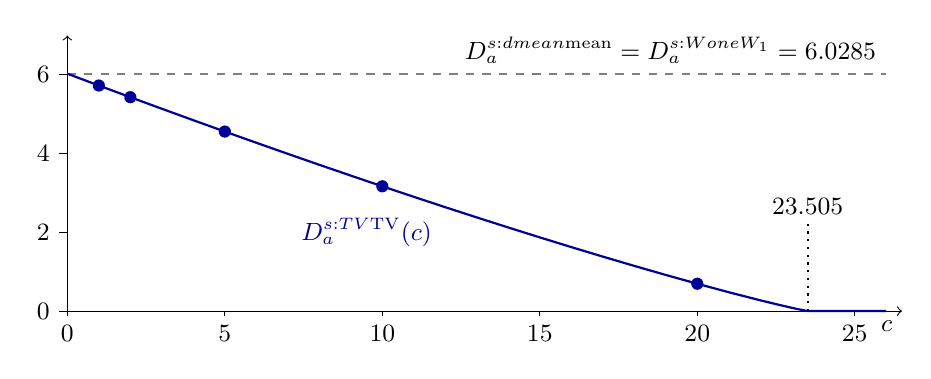
\begin{tikzpicture}[x=0.4cm,y=0.5cm]
  \draw[->] (0,0) -- (26.5,0) node[below left] {\small $c$};
  \draw[->] (0,0) -- (0,7.0);
  \foreach \x in {0,5,10,15,20,25} \draw (\x,0) -- (\x,-0.12) node[below] {\small \x};
  \foreach \y in {0,2,4,6} \draw (0,\y) -- (-0.25,\y) node[left] {\small \y};
  \draw[dashed,thick,gray] (0,6.0285) -- (26,6.0285)
    node[above left,black] {\small $D^{\dmean}_a=D^{\Wone}_a=6.0285$};
  \draw[thick,blue!60!black] plot coordinates {(0,6.0285) (1,5.7289) (2,5.4322) (3,5.1383)
    (4,4.8474) (5,4.5595) (6,4.2748) (7,3.9933) (8,3.7151) (9,3.4404) (10,3.1692) (11,2.9017)
    (12,2.6380) (13,2.3782) (14,2.1227) (15,1.8715) (16,1.6250) (17,1.3835) (18,1.1474)
    (19,0.9173) (20,0.6940) (21,0.4786) (22,0.2733) (22.5,0.1757) (23,0.0831) (23.25,0.0397)
    (23.505,0)} -- (26,0);
  \foreach \p in {(1,5.7289),(2,5.4322),(5,4.5595),(10,3.1692),(20,0.6940)}
    \fill[blue!60!black] \p circle (2.2pt);
  \draw[dotted,thick] (23.505,0) -- (23.505,2.2) node[above] {\small $23.505$};
  \node[blue!60!black] at (9.5,2.0) {\small $D^{\TV}_a(c)$};
\end{tikzpicture}
\caption{Example~\ref{ex:no-drift} ($S=\{0,\frac12,1\}$, $\nu_a=\nu'_a=(0.02,0.96,0.02)$,
$\mu^\star=0.6$, $L_a=0.11$): the optimal $\lim_T\E N_a(T)/\log T$ against the source rate
$c=\lim_T N'_a(T)/\log T$, with the mean drift or $W_1$ (dashed) and with total variation (solid;
dots: certified values of Table~\ref{tab:no-drift}; computation in Section~\ref{sec:numerics}).}
\label{fig:no-drift}
\end{figure}

\paragraph{Our contributions} We summarise our main contributions below.
\begin{enumerate}
\item[(i)] \emph{Algorithm.} The index policy \Alg{} (Definition~\ref{def:algo},
  Algorithm~\ref{alg:index}), whose index maximises the mean of a target law over the pairs of laws
  within the drift bound, inside one Kullback--Leibler budget for both samples; each index is a
  convex programme.
\item[(ii)] \emph{Regret upper bound and optimality.} \Alg{} attains $D_a(c_a)$, is never worse
  than KL-UCB on $S$ whatever the source sizes, and needs the drift condition on one optimal arm only
  (Theorem~\ref{thm:main}); paired with the known lower bound (Proposition~\ref{prop:lower}), it is
  asymptotically optimal (Corollary~\ref{cor:optimal}).
\item[(iii)] \emph{The constant.} Its supremum form~\eqref{eq:sup-form} (Lemma~\ref{lem:D}); the
  ordering from the mean gap to $W_1$, Kolmogorov and total variation
  (Proposition~\ref{prop:order}); exact criteria for a gain over the mean drift and over KL-UCB
  (Proposition~\ref{prop:criteria}); the threshold of $o(\log T)$ pulls
  (Proposition~\ref{prop:threshold}).
\item[(iv)] \emph{When the law helps.} Never for Bernoulli laws (Proposition~\ref{prop:bernoulli}),
  never for $W_1$ without drift (Proposition~\ref{prop:w1}), strictly for total variation when the
  source law must move and the projections differ at an interior atom (Proposition~\ref{prop:tv}).
\item[(v)] \emph{Examples and simulations.} Certified values of the constant on explicit
  instances, including one without drift where total variation transfers and the mean and $W_1$ do
  not (Section~\ref{sec:examples}), and a small simulation of \Alg{} against KL-UCB and
  KL-UCB-Transfer on that instance (Section~\ref{sec:experiments}).
\end{enumerate}

\paragraph{Outline} Section~\ref{sec:related} discusses related work. Section~\ref{sec:setting}
formalises the setting. Section~\ref{sec:lower} recalls the lower bound and explains the optimal
constant. Section~\ref{sec:algorithm} recalls KL-UCB and defines \Alg{}. Section~\ref{sec:main}
states its regret bound and its optimality, and Section~\ref{sec:structure} compares the constant
across distances. Section~\ref{sec:overview} explains how the proofs work,
Section~\ref{sec:examples} gives examples and simulations, Section~\ref{sec:conclusion} concludes and
Section~\ref{sec:open} states open questions. The proofs are in the appendices.

% ----------------------------------------------------------------
\section{Related work and context}\label{sec:related}\label{sec:closest}

Table~\ref{tab:comparison} compares the first-order results closest to ours. We discuss each line
of work below.

\paragraph{Transfer with a drift between means} \citet{PMM25} introduced the transfer model with a
known bound on a pseudo-distance between the source and target laws, proved the lower bound for an
arbitrary pseudo-distance and deterministic source sizes \citep[Theorem~3]{PMM25}, and introduced
the source-penalised index KL-UCB-Transfer \citep[Section~5.2, (4)]{PMM25}, the first form of ours,
with an upper bound for Gaussian laws and the mean gap only \citep[Theorem~6]{PMM25}.
\citet{PMRM26} treat laws on $[0,1]$, a mean drift and source data collected by an unknown adaptive
policy: a lower bound \citep[Theorem~2]{PMRM26} and an upper bound of KL-UCB-Transfer
\citep[Theorem~3]{PMRM26}, which match when the source sizes concentrate, except possibly at
the boundary $\mu'_a=\mu^\star-L_a$ \citep[Proposition~4]{PMRM26}, and an analysis of misspecification \citep[Theorem~5]{PMRM26}.

\paragraph{KL-UCB and laws on a finite support} Without source data, our index is KL-UCB with the
divergence computed on the known support. Empirical KL-UCB \citep[Theorem~2]{CGMMS13} attains the
constant $1/\Kinf(\nu_a,\mu^\star)$ for finitely supported laws on $[0,1]$; see also
\citet{BK96} for laws on a known finite support. The dual form of $\Kinf$ on a bounded support is
due to \citet[Theorems~5 and~8]{HT10}.

\paragraph{Historical and offline data} \citet{SJ12} show that a logarithmic amount of history from
the same laws can make the regret constant. With biased offline data, the bias is bounded through
the means only \citep[(4)]{CL24}, \citep{LFCK26}, and the algorithms cannot use a drift between
laws. See also \citet{KT26} for Wasserstein ambiguity sets used to borrow external data in clinical
trials, a testing problem.

\paragraph{Structured bandits} The index of OSLB and CKL-UCB \citep[Section~4.1]{MCP14} also
maximises a mean under one budget shared by several samples, but every sample comes from an arm
chosen by the learner (see also OSSB, \citealp[Section~5]{CMP17}); ours come from laws that are
not arms, in imposed numbers.

\begin{table}[t]
\centering\small
\caption{The closest published results. Here $c=\lim_TN'_a(T)/\log T$, and $\Kinf$ is the smallest
divergence to a law with a larger mean, in the model of the line.}
\label{tab:comparison}
\begin{tabular}{@{}p{0.21\textwidth}p{0.37\textwidth}p{0.34\textwidth}@{}}
\toprule
\raggedright Result & \raggedright Setting & Constant of $\E N_a(T)/\log T$\tabularnewline
\midrule
\raggedright Empirical KL-UCB, \citet[Thm.~2]{CGMMS13} & \raggedright no source; finitely supported
laws on $[0,1]$, $\mu^\star<1$ & upper bound $1/\Kinf(\nu_a,\mu^\star)$\tabularnewline
\raggedright \citet[Thm.~3]{PMM25} & \raggedright pseudo-distance $d$, $d(\nu_k,\nu'_k)\le L_k$;
deterministic sizes & lower bound; on a finite support, $D_a(c)$ (Prop.~\ref{prop:lower})\tabularnewline
\raggedright KL-UCB-Transfer, \citet[Thm.~6]{PMM25} & \raggedright Gaussian laws, mean gap;
deterministic sizes & upper bound, mean-drift constant\tabularnewline
\raggedright KL-UCB-Transfer, \citet[Thms.~2,~3]{PMRM26} & \raggedright laws on $[0,1]$, mean gap;
source data from an adaptive policy & lower and upper bounds,
$(1-c\,\Kinf(\nu'_a,\mu^\star-L_a))_+/\Kinf(\nu_a,\mu^\star)$\tabularnewline
\raggedright \Alg{} (this paper) & \raggedright laws on a known finite $S$; an integral
probability metric $d$ ($\TV$, $\KSd$, $\Wone$, mean gap); deterministic sizes & upper bound
$D_a(c)$, with $D^{\TV}_a\le D^{\KSd}_a\le D^{\Wone}_a\le D^{\dmean}_a$\tabularnewline
\bottomrule
\end{tabular}
\end{table}

\paragraph{Closest related work} None of the results of Table~\ref{tab:comparison} gives
Theorem~\ref{thm:main}, for the following reasons.
\begin{itemize}
\item \emph{The lower bound} \citep[Theorem~3]{PMM25} holds for a general pseudo-distance and
  deterministic sizes; Proposition~\ref{prop:lower} is a variant of it on laws carried by $S$, and
  Lemma~\ref{lem:D} identifies its constant with~\eqref{eq:sup-form}. It is a lower bound and gives
  no algorithm; the upper bound of the same paper \citep[Theorem~6]{PMM25} is for Gaussian laws and
  the mean gap only.
\item \emph{The mean drift} \citep{PMRM26}: KL-UCB-Transfer reads the source sample through a mean
  constraint only. On our instances its guarantee is the mean-drift constant
  $D^{\dmean}_a(c_a)$, which exceeds the lower bound $D^d_a(c_a)$ exactly in the cases of
  Proposition~\ref{prop:criteria} (Section~\ref{sec:mean-drift}).
\item \emph{KL-UCB} \citep{CGMMS13} is the case without source data.
\item \emph{Historical data without drift} \citep{SJ12}: this is Proposition~\ref{prop:threshold}
  without drift; the drift adds the threshold $1/G^d$, which depends on $d$ and $L_a$, and the
  constant below it.
\item \emph{Structured bandits} \citep{MCP14,CMP17} and \emph{biased offline data}
  \citep{CL24,LFCK26}: the samples are pulled by the learner, or the bias is bounded through the
  means only.
\end{itemize}

\paragraph{Gap with the literature} For a drift measured between laws, a lower bound was known
\citep[Theorem~3]{PMM25} but no algorithm attaining it, and no description of its constant: when it
is smaller than with a mean drift, when it vanishes, and how it depends on the distance. What is new
here, as far as we found, is the index policy \Alg{} with its optimality on a known finite support,
the structure results of Section~\ref{sec:structure}, and the examples where a distance between laws
transfers and the mean does not.

\paragraph{Techniques} The upper bound follows the analysis of KL-UCB of \citet{CGMMS13} with the
method of types \citep[see][]{CK11}; the source of the optimal arm is handled with a margin, as in
\citet[Lemma~17]{PMRM26}, and that of the suboptimal arm by lower semicontinuity. The lower bound is
the change of measure of \citet[(6)]{GMS19} with the source samples as forced pulls, as in substance
in \citet[Appendix~A]{PMM25}. Appendix~\ref{sec:attribution} lists the sources of each technique.

% ----------------------------------------------------------------
\section{Problem formulation}\label{sec:setting}

In this section we introduce the setting, first the laws on a finite support and the classical
bandit, then the distances between laws and the transfer setting. The model follows
\citet{PMM25,PMRM26}. The drift is measured by a pseudo-distance between laws. The rewards take
values in a known finite set $S$ and the source sizes are deterministic, as the analysis uses the
method of types. Consistency is required for one sequence of source sizes only
(Definition~\ref{def:class}), which makes the lower bound stronger.

\subsection{Classical setting}

\begin{definition}[Laws on a finite support]\label{def:laws}
Let $S\subset[0,1]$ be a finite set with $|S|\ge2$. Its largest point is $\dt{s:xmax}x_{\max}:=\max S$
and its smallest point is $\dt{s:xmin}x_{\min}:=\min S$. The set of probability vectors on $S$ is
\begin{equation*}
\dt{s:simp}\mathcal P_S:=\Big\{q=(q(y))_{y\in S}\in[0,\infty)^S:\ \sum_{y\in S}q(y)=1\Big\}.
\end{equation*}
For $q\in\Simp$, its mean, its support and its distribution function are
\begin{equation*}
\dt{s:mean}\mean(q):=\sum_{y\in S}q(y)\,y,\qquad
\dt{s:supp}\supp\,q:=\{y:q(y)>0\},\qquad
\dt{s:F}\Fd_q(s):=\sum_{y\le s}q(y).
\end{equation*}
For $r,q\in\Simp$, the Kullback--Leibler divergence is
\begin{equation*}
\dt{s:KL}\KL(r,q):=\sum_{y:r(y)>0}r(y)\log\frac{r(y)}{q(y)}\in[0,\infty],
\end{equation*}
with $\KL(r,q):=\infty$ if $q(y)=0<r(y)$ for some $y$. The total variation is
\begin{equation*}
\dt{s:TV}\TV(r,q):=\sum_{y}(r(y)-q(y))_+ .
\end{equation*}
For $\rho\in\Simp$ and $\ell\in\mathbb R$, the smallest divergence to a law of mean at least $\ell$ is
\begin{equation*}
\dt{s:Ks}\Ks(\rho,\ell):=\inf\{\KL(\rho,q):q\in\Simp,\ \mean(q)\ge\ell\},
\end{equation*}
with $\inf\emptyset:=\infty$. Products $0\cdot\infty$ are $0$, and $e^{-\infty}:=0$.
\end{definition}

In the classical stochastic bandit on $S$, $K$ arms have laws in $\Simp$; at each round the learner
pulls an arm and observes a reward drawn from its law. A learner that is consistent on the laws
carried by $S$ pulls a suboptimal arm $a$ about $\log T/\Ks(\nu_a,\mus)$ times at least
(Section~\ref{sec:lower}), and KL-UCB with the divergence computed on $S$ attains this constant
(Section~\ref{sec:algorithm} and Theorem~\ref{thm:main}(i) without source data). The transfer setting adds source samples whose laws are tied to the
target laws by a distance.

\subsection{Distances between laws}

\begin{definition}[Integral probability metric]\label{def:ipm}
\uses{def:laws}
Let $\mathcal F$ be a nonempty set of functions $S\to[0,1]$. For $q,q'\in\Simp$,
\begin{equation*}
\dt{s:dF}\dF(q,q'):=\sup_{f\in\mathcal F}\Big|\sum_{y\in S}f(y)(q(y)-q'(y))\Big|.
\end{equation*}
The four examples are:
\begin{itemize}
\item the total variation $d=\TV$, with $\mathcal F$ the set of all functions $S\to[0,1]$;
\item the Kolmogorov distance $\dt{s:KS}d=\mathrm{KS}$, with
  $\mathcal F=\{\ind_{(-\infty,s]}:s\in\mathbb R\}$, so that
  $\mathrm{KS}(q,q')=\max_s|\Fd_q(s)-\Fd_{q'}(s)|$;
\item the Wasserstein distance $\dt{s:Wone}d=\Wone$, with $\mathcal F$ the $1$-Lipschitz functions
  $S\to[0,1]$;
\item the mean gap $\dt{s:dmean}d=\mathrm{mean}$, with $\mathcal F=\{y\mapsto y\}$, so that
  $d(q,q')=|\mean(q)-\mean(q')|$.
\end{itemize}
The pseudo-distance $d$ has the \emph{mean property} \dt{s:M}\propM{} if $|\mean(q)-\mean(q')|\le d(q,q')$ for
all $q,q'\in\Simp$.
\end{definition}

The $\TV$ of Definition~\ref{def:ipm} is that of Definition~\ref{def:laws} (the supremum is attained
at $f=\ind_{\{q>q'\}}$, Lemma~\ref{lem:ipm}(c)), and its $\Wone$ is the usual Wasserstein distance
(Kantorovich--Rubinstein; not used). A \emph{pseudo-distance of Definition~\ref{def:ipm}} is any
$d=\dF$.

\subsection{Transfer learning setting}

\begin{definition}[Transfer bandit on $S$]\label{def:model}
\uses{def:laws}
There are $K\ge2$ arms. Arm $k$ has a target law $\nu_k\in\Simp$ and a source law $\nu'_k\in\Simp$.
The mean of arm $k$ is $\dt{s:mu}\mk_k:=\mean(\nu_k)$, and the best mean is
$\dt{s:mustar}\mus:=\max_k\mk_k$. The bounds $L_k>0$ are known. For each horizon $T$, the
source sizes $N'_k=N'_k(T)\in\mathbb N$ are deterministic.

The data are independent families:
\begin{itemize}
\item the source sample $X'_{k,1},\dots,X'_{k,N'_k}$, i.i.d.\ $\nu'_k$;
\item the stack $X_{k,1},X_{k,2},\dots$, i.i.d.\ $\nu_k$;
\item the randomisation variables $V_0,V_1,\dots$, i.i.d.\ uniform on $[0,1]$.
\end{itemize}
\dt{s:At}A learner chooses at round $t\ge1$ an arm $\At_t$ as a measurable function of the source
samples, of $V_0,\dots,V_{t-1}$ and of the past observations, and observes
$X_{\At_t,\Nc_{\At_t}(t)}$, where the number of pulls of arm $k$ up to round $t$ is
\begin{equation*}
\dt{s:N}\Nc_k(t):=\sum_{u\le t}\ind(\At_u=k).
\end{equation*}
\dt{s:hnu}The empirical laws are $\hnu_{k,s}$, that of $X_{k,1},\dots,X_{k,s}$;
$\hnu_k(t):=\hnu_{k,\Nc_k(t)}$; and $\hnu'_k$, that of the source sample of arm $k$ (any
fixed law if $N'_k=0$). The regret is
\begin{equation*}
\dt{s:R}\Reg_T:=\sum_k(\mus-\mk_k)\E \Nc_k(T).
\end{equation*}
\end{definition}

\begin{definition}[Class of instances; consistency]\label{def:class}
\uses{def:ipm, def:model}
The class of instances is
\begin{equation*}
\dt{s:Theta}\Thet:=\{(\nu,\nu')\in\Simp^K\times\Simp^K:\ d(\nu_k,\nu'_k)<L_k\text{ for every }k\}.
\end{equation*}
\dt{s:Cons}For a sequence of source sizes $N'=(N'(T))_T$, $\Cons(N')$ is the set of learners such
that, for every $(\nu,\nu')\in\Thet$, every arm $k$ with $\mk_k<\mus$ and every $\alpha>0$,
$\E \Nc_k(T)=o(T^\alpha)$ when the source sizes are $N'(T)$.
\end{definition}

\paragraph{Notational convention} Logarithms are natural, $a\wedge b:=\min(a,b)$,
$a\vee b:=\max(a,b)$ and $(x)_+:=\max(x,0)$. A law on $S$ is identified with its probability
vector, and \dt{s:dirac}$\mathbf 1_{\{x_{\max}\}}$ is the Dirac mass at $\xmax$. The mean of a
source law is $\dt{s:muprime}\mkp_k:=\mean(\nu'_k)$. A tilde, as in $\tilde\E$, marks an alternative
instance. Appendix~\ref{sec:notation} lists the symbols, each a link to its definition.

% ----------------------------------------------------------------
\section{Lower bound and the optimal constant}\label{sec:lower}

In this section we first recall the classical lower bound, then define the constant of the transfer
setting, state the lower bound for it and explain what it means.

\subsection{Lower bound in the classical setting}

Without source data, the lower bound of \citet{BK96} says that every
learner consistent on the laws carried by $S$ satisfies, for every arm $a$ with $\mk_a<\mus<\xmax$,
\begin{equation*}
\liminf_{T\to\infty}\frac{\E \Nc_a(T)}{\log T}\ge\frac{1}{\Ks(\nu_a,\mus)}.
\end{equation*}
To rule out an alternative law $q$ of arm $a$ with $\mean(q)>\mus$, the learner needs
$\log T/\KL(\nu_a,q)$ pulls of $a$, and $\Ks(\nu_a,\mus)$ is the divergence of the closest such
alternative. This is also the case without source of Proposition~\ref{prop:lower} below.

\subsection{The constant of the transfer setting}

With source data, an alternative must move the target law and the source law together, within the
drift bound. The following definition gives the resulting programme and its constant.

\begin{definition}[The constant]\label{def:constant}
\uses{def:laws, def:ipm, def:model, lem:projection}
For an arm $a$ and $\mu\in\mathbb R$, the set of alternative pairs is
\begin{equation*}
\dt{s:Gamma}\Gamma_a(\mu):=\{(q,q')\in\Simp^2:\ \mean(q)\ge\mu,\ d(q,q')\le L_a\}.
\end{equation*}
For $x,c\ge0$, the programme is
\begin{equation*}
\dt{s:J}\Jf_a(x,c;\mu):=\inf_{(q,q')\in\Gamma_a(\mu)}\big[x\,\KL(\nu_a,q)+c\,\KL(\nu'_a,q')\big].
\end{equation*}
Let $\Jf_a(x,c):=\Jf_a(x,c;\mus)$. The constant is
\begin{equation*}
\dt{s:D}\Dc_a(c):=\inf\{x>0:\ \Jf_a(x,c)\ge1\}.
\end{equation*}
Further, let $\dt{s:Kzero}\mathcal K_0:=\Ks(\nu_a,\mus)$ and
$\dt{s:Kzerop}\mathcal K'_0:=\Ks(\nu'_a,\mus-L_a)$. When $\mk_a<\mus<\xmax$, let
\dt{s:Qs}$Q^\star$ be the unique minimiser of $\KL(\nu_a,\cdot)$ on $\{q\in\Simp:\mean(q)\ge\mus\}$
and \dt{s:Qps}$Q'^\star$ the unique minimiser of $\KL(\nu'_a,\cdot)$ on
$\{q'\in\Simp:\mean(q')\ge\mus-L_a\}$ (they exist by Lemma~\ref{lem:projection}).
\end{definition}

In words, $\Jf_a(x,c)\log T$ is the least information that $x\log T$ pulls of $a$ and $c\log T$ source
samples collect against an alternative pair $(q,q')$ that makes $a$ optimal, and $\Dc_a(c)$ is the
least $x$ for which it reaches $\log T$. Section~\ref{sec:meaning} gives the supremum
form~\eqref{eq:sup-form}. The quantities $\Ko$, $\Kop$, $\Qs$, $\Qps$ do not depend on $d$.

\subsection{Lower bound in the transfer setting}

The following lower bound is a variant of \citet[Theorem~3]{PMM25}, stated on laws carried by $S$.

\begin{proposition}[Lower bound; a variant of {\citet[Theorem~3]{PMM25}}]\label{prop:lower}
\uses{def:laws, def:ipm, def:model, def:class, def:constant}
Let $\pi\in\Cons(N')$, $(\nu,\nu')\in\Thet$, and let $a$ be an arm with $\mk_a<\mus$ and
$\dt{s:cbar}\cbar_a:=\limsup_{T}N'_a(T)/\log T<\infty$. Then
\begin{equation*}
\liminf_{T\to\infty}\frac{\E \Nc_a(T)}{\log T}\ge \Dc_a(\cbar_a).
\end{equation*}
\end{proposition}

(See the proof in Appendix~\ref{sec:proof-lower}.)

\paragraph{Relation with \texorpdfstring{\citet{PMM25}}{Prevost et al. (2025)}} This bound is not
new: it is a variant of \citet[Theorem~3]{PMM25}, stated there for an arbitrary pseudo-distance and
deterministic sizes, with the same proof \citep[Appendix~A]{PMM25}. It is not literally a
specialisation. The class $\Cons(N')$ asks for consistency for one sequence of sizes only, on the
instances with the strict constraint $d<L$, so it contains more learners than the class of
\citet[Definition~2]{PMM25}, and the statement is slightly stronger in the class; the support is
finite, and the constraint set of Definition~\ref{def:constant} is closed. We prove it
(Appendix~\ref{sec:proof-lower}) because the identification with $\Dc_a$ (Lemma~\ref{lem:D}) is
needed to pair it with Theorem~\ref{thm:main}. It also applies to every learner of the class of
\citet[Section~4.2]{PMRM26} when $d$ has \propM{} (Appendix~\ref{sec:proof-lower}).

\subsection{What the constant means}\label{sec:meaning}

Assume $\mus<\xmax$. (If $\mus=\xmax$, then $\Dc_a\equiv0$ by Lemma~\ref{lem:D}: the
optimal mean is the largest point of $S$, which a learner can certify in $o(\log T)$ pulls.) By
Lemma~\ref{lem:D}(a) (\emph{the constant as a supremum}), $\Dc_a(c)$ is the
supremum~\eqref{eq:sup-form} of the ratio
\begin{equation*}
\Rat(q,q')=\frac{\big(1-c\,\KL(\nu'_a,q')\big)_+}{\KL(\nu_a,q)}
\end{equation*}
over the pairs with $\mean(q)>\mus$, $d(q,q')<L_a$ and finite divergences. Each such pair is an
alternative instance in which arm $a$ is the only optimal arm, as explained in the introduction
(Step~2 of the proof of Proposition~\ref{prop:lower} makes this precise). Two readings follow.

\paragraph{The two ends} Each ratio is at most $1/\KL(\nu_a,q)\le1/\Ko$. Hence
\begin{equation*}
\Dc_a(c)\le\frac1{\Ko},\qquad \Dc_a(0)=\frac1{\Ko},
\end{equation*}
the constant of KL-UCB on $S$: the source never hurts. Each ratio is a nonincreasing convex function
of $c$, so $\Dc_a$ is nonincreasing and convex (Figure~\ref{fig:no-drift}). It vanishes exactly when
$c\ge1/\Gd^d$, a threshold given by Proposition~\ref{prop:threshold}.

\paragraph{The mean gap} An alternative needs $\mean(q)\ge\mus$, hence $\KL(\nu_a,q)\ge\Ko$. Then,
for the mean gap, $\mean(q')\ge \mean(q)-L_a\ge\mus-L_a$, hence $\KL(\nu'_a,q')\ge\Kop$. The pair of
Kullback--Leibler projections $(\Qs,\Qps)$ attains both bounds, and it is feasible for the mean gap
when $\mean(\nu'_a)\le\mus+L_a$. So the target and source terms split, and
\begin{equation*}
\Dc^{\dmean}_a(c)=\frac{(1-c\Kop)_+}{\Ko}
\end{equation*}
(Proposition~\ref{prop:order}(a)), as in the mean-drift model of \citet{PMRM26}. With a distance
between laws, the pair of projections is feasible only if $d(\Qs,\Qps)\le L_a$. When it is not,
every feasible pair costs more, and $\Dc^d_a(c)<\Dc^{\dmean}_a(c)$ under the hypotheses of
Proposition~\ref{prop:criteria}(a).

% ----------------------------------------------------------------
\section{The algorithm}\label{sec:algorithm}

In this section we recall KL-UCB on a finite support and its transfer version for the mean drift,
then define \Alg{}.

\subsection{KL-UCB in the classical setting}

KL-UCB pulls at each round an arm whose index, an upper confidence bound on its mean, is maximal
\citep{CGMMS13}. On the known support $S$, the index of arm $k$ after round $t$ is
\begin{equation*}
\max\big\{\mean(q):\ q\in\Simp,\ \Nc_k(t)\,\KL(\hnu_k(t),q)\le\dl_t\big\},
\end{equation*}
for an exploration rate $\dl_t$ of order $\log t$. For the mean drift, KL-UCB-Transfer
\citep[Section~5.2]{PMRM26} adds the source sample: the candidate mean $\mu$ of the target law must be
compatible with the target observations and, through the mean constraint, with a source law of mean
at least $\mu-L_k$, inside one budget for both samples.

\subsection{\texorpdfstring{The algorithm \texttt{KL-UCB-$d$-Transfer}}{The algorithm KL-UCB-d-Transfer}}

We use the same template, with the drift constraint measured by $d$ between the two laws. The index
of arm $k$ is the largest mean of a target law $q$ that is plausible jointly with some source law
$q'$: the pair satisfies the drift bound $d(q,q')\le L_k$, and the information that the target and
source observations collect against it stays below the exploration rate.

\begin{definition}[KL-UCB-$d$-Transfer]\label{def:algo}
\uses{def:laws, def:ipm, def:model}
The inputs are $S$, $d$, $(L_k)_k$ and the source samples. The exploration rate is
\begin{equation}\label{eq:rate}
\dt{s:delta}\dl_t:=\log(t\vee3)+\log\log(t\vee3).
\end{equation}
At rounds $t=1,\dots,K$, pull arm $t$. \dt{s:U}At the end of every round $t\ge K$, compute for every
arm $k$
\begin{equation}\label{eq:index}
\Ix_k(t):=\max\Big\{\mean(q):\ (q,q')\in\Simp^2,\ d(q,q')\le L_k,\
\Nc_k(t)\,\KL(\hnu_k(t),q)+N'_k\,\KL(\hnu'_k,q')\le\dl_t\Big\},
\end{equation}
with $\max\emptyset:=-\infty$ and $N'_k\KL(\hnu'_k,q'):=0$ when $N'_k=0$. Then pull
$\At_{t+1}\in\arg\max_k\Ix_k(t)$, ties broken uniformly at random with $V_t$.
\end{definition}

The two samples share one budget, coupled by the distance: a source sample that is far from every
law within distance $L_k$ of a high-mean target law lowers the index.

\begin{algorithm}[t]
\caption{\texttt{KL-UCB-$d$-Transfer} (Definition~\ref{def:algo})}\label{alg:index}
\begin{algorithmic}[1]
\Require the support $S$, the pseudo-distance $d$, the bounds $L_1,\dots,L_K$, the source samples
  (sizes $N'_k$, empirical laws $\hnu'_k$)
\For{$t=1,\dots,K$}
  \State pull arm $t$ and observe its reward
\EndFor
\For{$t=K,K+1,\dots$}
  \For{every arm $k$}
    \State solve the convex programme~\eqref{eq:index} in $(q,q')\in\Simp^2$:
    \Statex \qquad $\Ix_k(t)\gets\max\{\mean(q):\ d(q,q')\le L_k,\
      \Nc_k(t)\KL(\hnu_k(t),q)+N'_k\KL(\hnu'_k,q')\le\dl_t\}$
  \EndFor
  \State pull $\At_{t+1}\in\arg\max_k\Ix_k(t)$, ties broken uniformly at random (with $V_t$)
  \State observe the reward; update $\Nc_{\At_{t+1}}(t+1)$ and $\hnu_{\At_{t+1}}(t+1)$
\EndFor
\end{algorithmic}
\end{algorithm}

\paragraph{Computation} The maximum is attained when the set is nonempty (Lemma~\ref{lem:index}).
The objective $\mean(q)$ is linear and the constraints are convex, since $\KL$ is convex in its second
argument and $d$ is jointly convex (Lemma~\ref{lem:ipm}(b)). So each index is a convex programme in
$2|S|$ variables, plus $O(|S|)$ slack variables for $\TV$, $\KSd$ and $\Wone$.

\paragraph{Without source data it is KL-UCB on $S$} If $N'_k=0$, the pair $(q,q)$ is feasible as
soon as $\Nc_k(t)\KL(\hnu_k(t),q)\le\dl_t$, so
\begin{equation*}
\Ix_k(t)=\max\{\mean(q):\Nc_k(t)\KL(\hnu_k(t),q)\le\dl_t\}.
\end{equation*}

\paragraph{Relation with KL-UCB-Transfer} With the one-sided mean condition $\mean(q)-\mean(q')\le L_k$ in
place of $d(q,q')\le L_k$, and $1\in S$, the index is that of KL-UCB-Transfer
\citep[Section~5.2]{PMRM26} with $\Kinf$ computed on $S$: for a fixed $\mean(q)=\mu$, the best $q'$ is
the KL projection of $\hnu'_k$ on $\{\mean(q')\ge\mu-L_k\}$. With the two-sided mean gap of
Definition~\ref{def:ipm}, the feasible set is smaller, so the index can be smaller than the
KL-UCB-Transfer index $U^{\rm KT}_k(t)$. The two coincide when
\begin{equation*}
\mean(\hnu'_k)\le U^{\rm KT}_k(t)+L_k :
\end{equation*}
at a maximiser of the one-sided programme, replace $q'$ by that projection at level
$U^{\rm KT}_k(t)-L_k$, whose mean is $\max(U^{\rm KT}_k(t)-L_k,\mean(\hnu'_k))$.

% ----------------------------------------------------------------
\section{Regret upper bound}\label{sec:main}\label{sec:upper}

In this section we state the regret bound of \Alg{} and its asymptotic optimality, then compare
them with the published bounds. In the classical setting, empirical KL-UCB satisfies, for every
suboptimal arm $a$ of a bandit with finitely supported laws on $[0,1]$ and $\mus<1$,
\begin{equation*}
\limsup_{T\to\infty}\frac{\E \Nc_a(T)}{\log T}\le\frac{1}{\Kinf(\nu_a,\mus)}
\end{equation*}
\citep[Theorem~2]{CGMMS13}, with $\Kinf$ computed over the finitely supported laws on $[0,1]$. For
laws carried by $S$ with $1\in S$, $\Kinf(\nu_a,\mus)=\Ks(\nu_a,\mus)$ (for a competitor $q$, apply
Lemma~\ref{lem:projection} on $S\cup\supp\,q$: the projection adds mass only at $1$), and this
matches the classical lower bound of Section~\ref{sec:lower}; otherwise $\Kinf(\nu_a,\mus)\le\Ks(\nu_a,\mus)$, and the bound
of empirical KL-UCB is no smaller than $1/\Ks(\nu_a,\mus)$. We obtain the following guarantee for \Alg{}; without source data, its
part~(i) is the same bound for KL-UCB with the divergence computed on the known support.

\begin{theorem}[Upper bound of KL-UCB-$d$-Transfer]\label{thm:main}
\uses{def:laws, def:ipm, def:model, def:constant, def:algo}
For every finite $S\subset[0,1]$ with $|S|\ge2$, every integral probability metric $d=\dF$
on $\Simp$ (Definition~\ref{def:ipm}), every $K\ge2$ and $L\in(0,\infty)^K$, every
$(\nu,\nu')\in\Simp^K\times\Simp^K$ such that some arm $i^\star$ with $\mk_{i^\star}=\mus$
satisfies $d(\nu_{i^\star},\nu'_{i^\star})<L_{i^\star}$ (no condition on the other arms), and with
deterministic source sizes $N'(T)\in\mathbb N^K$, the learner \Alg{} satisfies, for every arm $a$
with $\mk_a<\mus$:
\begin{enumerate}
\item[(i)] for every sequence of source sizes,
  \begin{equation*}
  \limsup_{T\to\infty}\frac{\E \Nc_a(T)}{\log T}\le\frac{1}{\Ks(\nu_a,\mus)}
  \end{equation*}
  (read as $0$ if $\Ks(\nu_a,\mus)=\infty$);
\item[(ii)] if $N'_a(T)/\log T\to c_a\in[0,\infty)$, then
  \begin{equation*}
  \limsup_{T\to\infty}\frac{\E \Nc_a(T)}{\log T}\le \Dc_a(c_a).
  \end{equation*}
\end{enumerate}
\end{theorem}

(See the proof in Appendix~\ref{sec:proof-upper}.)

\begin{corollary}[Asymptotic optimality]\label{cor:optimal}
\uses{def:class, def:constant, def:algo, thm:main, prop:lower}
Let $(\nu,\nu')\in\Thet$, and assume that $N'_k(T)/\log T\to c_k\in[0,\infty)$ for every arm $k$
with $\mk_k<\mus$. Then the learner \Alg{} belongs to $\Cons(N')$ for
every sequence $N'$, and, for every arm $a$ with $\mk_a<\mus$,
\begin{equation*}
\lim_{T\to\infty}\frac{\E \Nc_a(T)}{\log T}=\Dc_a(c_a).
\end{equation*}
Let $\dt{s:calR}\Rc:=\sum_{a:\mk_a<\mus}(\mus-\mk_a)\Dc_a(c_a)$. Then its regret
satisfies
\begin{equation*}
\lim_{T\to\infty}\frac{\Reg_T}{\log T}=\Rc,
\end{equation*}
and every $\pi\in\Cons(N')$ has
\begin{equation*}
\liminf_{T\to\infty}\frac{\Reg_T}{\log T}\ge\Rc .
\end{equation*}
\end{corollary}

(See the proof in Appendix~\ref{sec:proof-upper}.)

\paragraph{Comparison with the lower bound} Corollary~\ref{cor:optimal} pairs the upper bound of
Theorem~\ref{thm:main}(ii) with the lower bound of Proposition~\ref{prop:lower} in the same class,
the learners of $\Cons(N')$: the constant $\Dc_a(c_a)$ cannot be improved, and \Alg{} attains it on
every instance of $\Thet$ whose source sizes have a rate.

\paragraph{Safety} Part~(i) is a safety guarantee: whatever the source sizes, even much larger than
$\log T$, and whatever the source laws of the arms other than $i^\star$, the learner is never worse
at first order than KL-UCB on the known support $S$. Part~(ii) is the transfer gain. Since
$\Dc_a(c)\le1/\Ko$ (Lemma~\ref{lem:D}), it improves on~(i) exactly when the source helps, and
Section~\ref{sec:structure} says when this happens. The drift condition is needed on one optimal
arm only.

\paragraph{Nature of the constants} The bounds are first order. The proof gives an explicit
non-asymptotic bound for the term of the optimal arm, of order $\Cone\Ctwo\log\log T$, with $\Cone$
and $\Ctwo$ depending on $|S|$, on the margin $L_{i^\star}-d(\nu_{i^\star},\nu'_{i^\star})$ and on
$\nu_{i^\star},\nu'_{i^\star}$, and, for $\Ctwo$, on the parameter $\varepsilon$ of the proof
(through $\thet=\min(\varepsilon,\etam/2)$, Definition~\ref{def:proof-notation} and
Lemma~\ref{lem:optimal-arm}). The term of the suboptimal arm comes from a lower-semicontinuity
argument and has no explicit rate (Lemma~\ref{lem:sub-constant}).

\paragraph{Scope} The laws are carried by a known finite set $S$, because the proof uses the method
of types; the model of all laws on $[0,1]$ is Open question~\ref{oq:nonparametric}. The source sizes
are deterministic (random sizes: Open question~\ref{oq:random}). The bounds are first order (Open
question~\ref{oq:second-order}). Nothing is claimed when the drift bound fails on every optimal arm
(Open question~\ref{oq:misspecification}). The distance is an integral probability metric with test
functions valued in $[0,1]$; the Hellinger distance and a Kullback--Leibler divergence between the
source and target laws are not covered.

\subsection{Comparison with published bounds}\label{sec:mean-drift}

\paragraph{Comparison with KL-UCB-Transfer} For laws on $[0,1]$, source data generated by an
adaptive policy and $|\mk_k-\mkp_k|<L_k$ for every arm, \citet[Theorems~2 and~3]{PMRM26} are a lower
bound and an upper bound of KL-UCB-Transfer, which match when the source sizes concentrate,
except possibly when $\mkp_a=\mus-L_a$ \citep[Proposition~4]{PMRM26} (for deterministic sizes
this boundary case is settled in Appendix~\ref{sec:degenerate}). If $d$ has \propM{}, our instances satisfy $|\mk_k-\mkp_k|<L_k$, and
\citet[Theorem~3]{PMRM26} gives KL-UCB-Transfer the constant
\begin{equation*}
\frac{(1-c_a\Kop)_+}{\Ko}=\Dc^{\dmean}_a(c_a)
\end{equation*}
when $1\in S$ (Proposition~\ref{prop:order}(a)). Here $\Kinf$ on $[0,1]$ equals $\Ks$ on laws
carried by $S$, because the projection on a bounded support adds mass only at $1$
(\citealp[Theorem~8 and its proof]{HT10}; for finitely supported competitors this is
Lemma~\ref{lem:projection}).

This is Theorem~\ref{thm:main}(ii) exactly when $\Dc^d_a(c_a)=\Dc^{\dmean}_a(c_a)$, and
Proposition~\ref{prop:criteria} (\emph{criteria for a gain}) says when it is not: exactly when
$d(\Qs,\Qps)>L_a$ or $d(\Qs,\nu'_a)>L_a$. There KL-UCB-Transfer, which reads the source sample
through a mean constraint only, is guaranteed the mean constant only, strictly above the lower bound
$\Dc^d_a(c_a)$. Example~\ref{ex:no-drift} is such a case, with $d=\TV$.

\paragraph{The drift on one optimal arm only} For the mean drift, the analysis of misspecification
\citep[Theorem~5]{PMRM26}, with its parameter $\mu^\dagger$ equal to the optimal mean, already needs
only $\mus<\mkp_1+L_1$ on the optimal arm~$1$. The condition of Theorem~\ref{thm:main} on one
optimal arm is its analogue for a distance between laws, in a two-sided form; it is not new for the
mean gap.
% ----------------------------------------------------------------
\section{When does the law help?}\label{sec:structure}

In this section the constant is compared across pseudo-distances, so no drift condition
$d(\nu_a,\nu'_a)<L_a$ for a fixed $d$ is assumed: each statement gives its hypotheses on the
instance. A superscript ($\Dc^{\TV}_a$, $\Dc^{\Wone}_a$, $\Dc^{\dmean}_a$, \dots) names the pseudo-distance
of Definition~\ref{def:ipm} used in $\Pairs_a$, $\Jf_a$ and $\Dc_a$. The quantities $\Ko$, $\Kop$, $\Qs$,
$\Qps$ are those of Definition~\ref{def:constant}: $\Qs$ is the KL projection of $\nu_a$ on
$\{\mean(q)\ge\mus\}$ and $\Qps$ that of $\nu'_a$ on $\{\mean(q')\ge\mus-L_a\}$. The four examples
of Definition~\ref{def:ipm} have the mean property \propM{} (Lemma~\ref{lem:ipm-order}).

The hypothesis $\mean(\nu'_a)\le\mus+L_a$ used below holds whenever $d(\nu_a,\nu'_a)<L_a$ for some
$d$ with \propM{}, since then
\begin{equation*}
\mean(\nu'_a)<\mk_a+L_a<\mus+L_a .
\end{equation*}
So it holds on $\Thet$ whenever the $d$ defining $\Thet$ has \propM{}, and in all the examples of
Section~\ref{sec:examples}.

\paragraph{In short}
\begin{itemize}
\item The constant is ordered: $\Dc^{\TV}_a\le \Dc^{\KSd}_a\le \Dc^{\Wone}_a\le \Dc^{\dmean}_a$, and
  $\Dc^{\dmean}_a=(1-c\Kop)_+/\Ko$ when $\mean(\nu'_a)\le\mus+L_a$
  (Proposition~\ref{prop:order}).
\item A distance between laws beats the mean exactly when it separates the two KL projections,
  $d(\Qs,\Qps)>L_a$, and the source helps at all exactly when $d(\Qs,\nu'_a)>L_a$
  (Proposition~\ref{prop:criteria}).
\item The constant is $0$ exactly when $c\ge1/\Gd^d$ (Proposition~\ref{prop:threshold}).
\item Bernoulli laws gain nothing (Proposition~\ref{prop:bernoulli}), nor does $\Wone$ when the
  source law equals the target law (Proposition~\ref{prop:w1}); total variation gains strictly as
  soon as the source law must move and the projections differ at an interior atom
  (Proposition~\ref{prop:tv}).
\end{itemize}

\subsection{Ordering and criteria}

\begin{proposition}[Ordering]\label{prop:order}
\uses{def:ipm, def:constant}
Let $L\in(0,\infty)^K$, $(\nu,\nu')\in\Simp^K\times\Simp^K$, and let $a$ be an arm with
$\mk_a<\mus<\xmax$. Then:
\begin{enumerate}
\item[(a)] if $\mean(\nu'_a)\le\mus+L_a$, then $\Dc^{\dmean}_a(c)=(1-c\Kop)_+/\Ko$ for every $c\ge0$;
\item[(b)] $\Dc^d_a\le \Dc^{\dmean}_a$ for every $d$ with \propM{};
\item[(c)] $\Dc^{\TV}_a\le \Dc^{\KSd}_a\le \Dc^{\Wone}_a\le \Dc^{\dmean}_a$.
\end{enumerate}
\end{proposition}

(See the proof in Subsection~\ref{sec:proof-prop-order}.)

\paragraph{The hypothesis of (a)} It cannot be dropped: if $\mean(\nu'_a)>\mus+L_a$, then $\Kop=0$
while $\Dc^{\dmean}_a(c)<1/\Ko$ for every $c>0$, by Proposition~\ref{prop:criteria}(b) with the mean
gap.

\begin{proposition}[Criteria]\label{prop:criteria}
\uses{def:ipm, def:constant}
Let $L\in(0,\infty)^K$, $(\nu,\nu')\in\Simp^K\times\Simp^K$, let $a$ be an arm with
$\mk_a<\mus<\xmax$, and let $c>0$. Then:
\begin{enumerate}
\item[(a)] if $d$ has \propM{}, $\mean(\nu'_a)\le\mus+L_a$ and $c\Kop<1$, then $\Dc^d_a(c)<\Dc^{\dmean}_a(c)$
  if and only if $d(\Qs,\Qps)>L_a$;
\item[(b)] for every $d$, $\Dc^d_a(c)<1/\Ko$ (the source helps at all) if and only if
  $d(\Qs,\nu'_a)>L_a$; for the mean gap this reads $|\mean(\nu'_a)-\mus|>L_a$, that is
  $\mean(\nu'_a)<\mus-L_a$ when $\mean(\nu'_a)\le\mus+L_a$.
\end{enumerate}
\end{proposition}

(See the proof in Subsection~\ref{sec:proof-prop-criteria}.)

\paragraph{Comparison with the mean drift} For the mean gap, (b) is the condition
$\mkp_a<\mus-L_a$ under which the source improves on KL-UCB in the mean-drift model
\citep[Section~6]{PMRM26}. Part~(a) is new: it says that a distance between laws improves on the
mean drift exactly when the pair of Kullback--Leibler projections violates the drift bound.

\subsection{The threshold of \texorpdfstring{$o(\log T)$}{o(log T)} pulls}

\begin{proposition}[Threshold of $o(\log T)$]\label{prop:threshold}
\uses{def:ipm, def:constant}
Let $L\in(0,\infty)^K$, $(\nu,\nu')\in\Simp^K\times\Simp^K$, and let $a$ be an arm with
$\mk_a<\mus<\xmax$. For $q'\in\Simp$, let
\begin{equation*}
\dt{s:omega}\om_d(q'):=\max\{\mean(q)-\mean(q'):q\in\Simp,\ d(q,q')\le L_a\},
\end{equation*}
and let
\begin{equation*}
\dt{s:G}\Gd^d:=\min\{\KL(\nu'_a,q'):q'\in\Simp,\ \mean(q')+\om_d(q')\ge\mus\}.
\end{equation*}
Then:
\begin{enumerate}
\item[(a)] for $c\ge0$, $\Dc^d_a(c)=0$ if and only if $c\,\Gd^d\ge1$;
\item[(b)] for the mean gap and for $\Wone$, $\om_d(q')=\min(L_a,\xmax-\mean(q'))$ and $\Gd^d=\Kop$;
\item[(c)] for total variation,
  $\om_{\TV}(q')=\max\{\sum_{y}\alpha(y)(\xmax-y):0\le\alpha\le q',\ \sum_y\alpha(y)\le L_a\}$.
\end{enumerate}
\end{proposition}

(See the proof in Subsection~\ref{sec:proof-prop-threshold}.)

\paragraph{Interpretation} The quantity $\om_d(q')$ is the largest increase of the mean that the
drift bound allows from a source law $q'$, and $\Gd^d$ is the divergence of the closest source law
from which a target law of mean $\mus$ is within reach. Above the rate $1/\Gd^d$, the source
samples alone rule out every alternative, and arm $a$ is pulled $o(\log T)$ times. For the mean gap
and $\Wone$ the threshold is that of the mean drift. Total variation can lower it: a mass moved
within the drift bound raises the mean by its size times the distance it travels to $\xmax$, so the
reachable means depend on the shape of $q'$ (Example~\ref{ex:no-drift}: $1/\Gd^{\TV}=23.505$, while
$\Kop=0$).

\subsection{Three special cases}

\begin{proposition}[Bernoulli laws: no gain]\label{prop:bernoulli}
\uses{def:ipm, def:constant}
Let $L\in(0,\infty)^K$, $(\nu,\nu')\in\Simp^K\times\Simp^K$, and let $a$ be an arm with
$\mk_a<\mus<\xmax$ and $\mean(\nu'_a)\le\mus+L_a$. If $\{0,1\}\subset S$ and $\nu_a,\nu'_a$ are
carried by $\{0,1\}$, then $\Dc^d_a=\Dc^{\dmean}_a$ for every $d$ with \propM{}.
\end{proposition}

(See the proof in Subsection~\ref{sec:proof-prop-bernoulli}.)

\begin{proposition}[$\Wone$: no gain without drift]\label{prop:w1}
\uses{def:ipm, def:constant}
Let $L\in(0,\infty)^K$, $(\nu,\nu')\in\Simp^K\times\Simp^K$, and let $a$ be an arm with
$\mk_a<\mus<\xmax$. If $\nu'_a=\nu_a$, then $\Dc^{\Wone}_a(c)=\Dc^{\dmean}_a(c)$ for every $c\ge0$.
\end{proposition}

(See the proof in Subsection~\ref{sec:proof-prop-w1}.)

\begin{proposition}[Total variation: strict gain]\label{prop:tv}
\uses{def:ipm, def:constant}
Let $L\in(0,\infty)^K$, $(\nu,\nu')\in\Simp^K\times\Simp^K$, and let $a$ be an arm with
$\mk_a<\mus<\xmax$. Assume $\Kop>0$. Then:
\begin{enumerate}
\item[(a)] $\TV(\Qs,\Qps)\ge L_a/(\xmax-\xmin)$, with equality only if $\Qs-\Qps$ is carried by
  $\{\xmin,\xmax\}$;
\item[(b)] hence $\Dc^{\TV}_a(c)<\Dc^{\dmean}_a(c)$ for every $c\in(0,1/\Kop)$ as soon as
  $\xmax-\xmin<1$ or $\Qs(y)\ne\Qps(y)$ for some $y\in S$ with $\xmin<y<\xmax$;
\item[(c)] this holds in particular when $\nu'_a=\nu_a$ and $\nu_a$ charges two points of
  $(\xmin,\xmax)$.
\end{enumerate}
\end{proposition}

(See the proof in Subsection~\ref{sec:proof-prop-tv}.)

\paragraph{Interpretation} The mean model loses exactly the information of the source law that the
projections use. $\Wone$ sees only displacements of mass, which a projection along the mean does not
create when the two laws coincide; total variation sees any reallocation.
Section~\ref{sec:examples} gives an instance where $\Dc^{\dmean}_a=\Dc^{\Wone}_a=6.03$ for every $c$,
while $\Dc^{\TV}_a=4.56$ at $c=5$ and $\Dc^{\TV}_a=0$ for $c\ge23.505$.

% ----------------------------------------------------------------
\section{How the proofs work}\label{sec:overview}

In this section we explain how the results are proved: the upper bound in detail, then the lower
bound and the structure results, and we give a map of the appendices.

\subsection{The upper bound}\label{sec:overview-upper}

Fix the instance, an optimal arm $i^\star$ with the margin
$\etam=\min\{1,L_{i^\star}-d(\nu_{i^\star},\nu'_{i^\star})\}>0$, a suboptimal arm $a$, and a small
$\varepsilon>0$ (Definition~\ref{def:proof-notation}). Let $\cA_T$ count the rounds at which the
index of $i^\star$ is below $\mus-\varepsilon$, and $\cB_T$ the pulls of $a$ at which the index
of $a$ is at least $\mus-\varepsilon$. A pull of $a$ needs one of the two, so
\begin{equation*}
\Nc_a(T)\le1+\cA_T+\cB_T
\end{equation*}
(Lemma~\ref{lem:decomposition}, the decomposition). The proof bounds each term in expectation.

\paragraph{Step 1: the index of the optimal arm is rarely too low} Lemma~\ref{lem:optimal-arm}
shows, for every $T\ge3$ and every sequence of source sizes,
\begin{equation*}
\E\cA_T\le\Cone\big(1+\Ctwo(1+\log\log T)\big).
\end{equation*}
The index of $i^\star$ is too low only if no pair $(q,q')$ with $q$ close to $\nu_{i^\star}$ is
feasible in it, and the proof exhibits one. Let $\qbar'$ be the empirical source law of $i^\star$
when it is within $\etam/2$ of $\nu'_{i^\star}$ in $d$, and the mixture
$(1-\frac\etam2)\nu'_{i^\star}+\frac\etam2\hnu'_{i^\star}$ otherwise (Lemma~\ref{lem:source}).
Then $d(\qbar',\nu'_{i^\star})\le\etam/2$, so every $q$ with $d(q,\nu_{i^\star})\le\etam/2$
satisfies $d(q,\qbar')\le L_{i^\star}$, by the triangle inequality and the margin $\etam$.

The cost of the source sample in this pair is $\Lam=N'_{i^\star}\KL(\hnu'_{i^\star},\qbar')$,
and its exponential moment is bounded uniformly in $N'_{i^\star}$:
\begin{equation*}
\E e^{\Lam}\le\Cone .
\end{equation*}
The pair is built from the unknown $\nu'_{i^\star}$, but it is only shown to be feasible; the
learner never computes it. The target term is controlled by a deviation inequality under a
$d$-constraint (Lemma~\ref{lem:deviation}), proved by the method of types: mixing an infeasible type
$r$ with $\nu_{i^\star}$ gives a feasible law and a gain $\thet\KL(r,\nu_{i^\star})$ in the exponent.

\paragraph{Step 2: the index of the suboptimal arm is rarely high} At a pull of $a$ counted in
$\cB_T$, the maximiser of the index of $a$ is a pair of $\Pairs_a(\mus-\varepsilon)$ with
objective at most $\dl_T$. As $\Nc_a$ increases at each pull, Lemma~\ref{lem:sub-reduction} gives
\begin{equation*}
\cB_T\le\sum_{s\le T}\ind(\Ph_s\le\dl_T),\qquad
\Ph_s=\min_{(q,q')\in\Pairs_a(\mus-\varepsilon)}\big[s\KL(\hnu_{a,s},q)+N'_a\KL(\hnu'_a,q')\big].
\end{equation*}
Dropping the source term gives the count $\cBz_T$ of KL-UCB, and Lemma~\ref{lem:sub-kl} bounds
\begin{equation*}
\E\cBz_T\le\frac{\dl_T}{\Ke-\xi}+\Cthree,\qquad\Ke=\Ks(\nu_a,\mus-\varepsilon):
\end{equation*}
this proves~(i). For~(ii), Lemma~\ref{lem:sub-constant} keeps the source term. Let $D:=\Dc_a(c_a)$ and
$\gamma>0$. For $s\ge(D+\gamma)\log T$, homogeneity gives
\begin{equation*}
\Ph_s\ge\log T\cdot\psif\Big(\hnu_{a,s},\hnu'_a,\frac{N'_a}{\log T},\mus-\varepsilon\Big),
\qquad
\psif(r,r',\beta,\mu)=\min_{(q,q')\in\Pairs_a(\mu)}\big[(D+\gamma)\KL(r,q)+\beta\KL(r',q')\big].
\end{equation*}
The function $\psif$ is lower semicontinuous, and, by Lemma~\ref{lem:D}(b) (\emph{the margin above
the constant}),
\begin{equation*}
\psif(\nu_a,\nu'_a,c_a,\mus)=\Jf_a(D+\gamma,c_a)\ge1+\gamma\Ko .
\end{equation*}
So $\psif>1+\gamma\Ko/2$ near this point, and the empirical laws $\hnu_{a,s}$ and $\hnu'_a$ are
near $\nu_a$ and $\nu'_a$ except on events of summable or vanishing probability. Hence
\begin{equation*}
\E\cB_T\le(D+\gamma)\log T+o(\log T).
\end{equation*}

\paragraph{Step 3: the combination} Part~(i) of Theorem~\ref{thm:main} sums the bounds of Steps~1
and~2 without the source term and lets $\xi$, then $\varepsilon$, tend to $0$; the lower
semicontinuity of $\ell\mapsto\Ks(\nu_a,\ell)$ gives the limit $\Ko$. Part~(ii) takes $\varepsilon$
small enough for Lemma~\ref{lem:sub-constant}, then lets $\gamma\to0$. The proof is in
Appendix~\ref{sec:proof-upper}.

\subsection{Where the difficulty lies}\label{sec:weak}

The KL-UCB part of the argument (the target sample of the optimal arm in $\cA_T$, and the count
$\cBz_T$) is the analysis of \citet{CGMMS13} on a finite support, with the method of types in place
of their deviation inequalities. Three steps are specific to transfer.
\begin{enumerate}
\item \emph{The neighbourhood step of Lemma~\ref{lem:sub-constant}}: the lower semicontinuity of
  $\psif$ jointly in $(r,r',\beta,\mu)$, where the constraint set depends on $\mu$ through a closed
  graph, and the use of $\TV$-neighbourhoods for both empirical laws. It is the only place where the
  source sample of the suboptimal arm enters, and it gives no rate; it affects
  Theorem~\ref{thm:main}(ii) only, not~(i).
\item \emph{The event inclusion of Lemma~\ref{lem:optimal-arm}}: it uses the analysis pair
  $(q,\qbar')$ built from the unknown $\nu'_{i^\star}$, and the independence of the stack of
  $i^\star$ from its source sample, which holds because the source sizes are deterministic. The
  margin $\etam$ is why the theorem asks for a strict inequality on the optimal arm.
\item \emph{The perturbation arguments of Lemmas~\ref{lem:J-zero} and~\ref{lem:D}} (mixing with
  $\dirac$ and with a common law): short but delicate; they need $\mus<\xmax$, and the case
  $\mus=\xmax$ is treated separately.
\end{enumerate}

\subsection{The lower bound and the structure results}

Proposition~\ref{prop:lower} is proved in Appendix~\ref{sec:proof-lower} by the change of measure of
\citet[(6)]{GMS19} (Lemma~\ref{cite:GMS19-6}), with the source samples written as forced pulls of
$K$ extra arms: an alternative pair $(q,q')$ of~\eqref{eq:sup-form} costs the divergence
$N'_a\KL(\nu'_a,q')+\E \Nc_a(T)\KL(\nu_a,q)$. The propositions of Section~\ref{sec:structure} are
proved in Appendix~\ref{sec:proof-structure} from the properties of $\Jf_a$
(Appendix~\ref{sec:proof-J}) and of the KL projection (Lemma~\ref{lem:projection}). The key tool is
Lemma~\ref{lem:criterion-point} (\emph{criterion at a point}): if $\Jf^d(x_0,c)\ge1$, then
$\Dc^d(c)<x_0$ if and only if $\Jf^d(x_0,c)>1$; at $x_0=\Dc^{\dmean}(c)$ it reduces
Proposition~\ref{prop:criteria}(a) to the question whether the pair of projections is feasible.

\subsection{Map of the appendices}\label{sec:map}

\begin{itemize}
\item Appendix~\ref{sec:cited}: the two results of \citet{GMS19} used for the lower bound, in the
  notation of this paper.
\item Appendix~\ref{sec:proofs}: tools on $\Simp$ (integral probability metrics, lower
  semicontinuity, the method of types, the KL projection, the likelihood-ratio order).
\item Appendix~\ref{sec:proof-J}: the programme $\Jf_a$, the supremum form of $\Dc_a$, and the attainment
  of the index.
\item Appendix~\ref{sec:proof-upper}: the proof of Theorem~\ref{thm:main} and
  Corollary~\ref{cor:optimal}: the decomposition, one lemma per term, concentration.
\item Appendix~\ref{sec:proof-lower}: the proof of Proposition~\ref{prop:lower}.
\item Appendix~\ref{sec:proof-structure}: the proofs of the structure results.
\item Appendix~\ref{sec:proof-duality}: the weak duality behind the numerical certificates, and
  their precision.
\item Appendix~\ref{sec:degenerate}: two further examples and the degenerate cases.
\item Appendices~\ref{sec:attribution} and~\ref{sec:notation}: the sources of the techniques and the
  notation.
\end{itemize}

% ----------------------------------------------------------------
\section{Examples and numerical experiments}\label{sec:examples}\label{sec:sanity}

In this section we say how the values of the constant are computed (Section~\ref{sec:numerics}),
give the instance without drift of Figure~\ref{fig:no-drift} and a complete two-armed instance that
satisfies all the hypotheses at once, and simulate \Alg{} on the latter against KL-UCB and
KL-UCB-Transfer (Section~\ref{sec:experiments}). Two further examples (Bernoulli laws, and a gain of
$\Wone$ over the mean with drift) and the degenerate cases (no source, the mean gap at the boundary
of the mean-drift model, $\mus=\xmax$, infinite divergences, ties) are in
Appendix~\ref{sec:degenerate}.

\subsection{Numerical setup}\label{sec:numerics}

\paragraph{Setup} The values below were computed by solving the convex programme $\Jf_a$ numerically
(slack variables for the absolute values) and bisecting on $x$. The two certificates are:
\begin{itemize}
\item a feasible pair with objective $<1$ certifies $\Jf_a(x,c)<1$, hence $\Dc_a(c)\ge x$;
\item a dual point of Lemma~\ref{lem:weak-duality} (\emph{weak duality}) with value $\ge1$
  certifies $\Jf_a(x,c)\ge1$, hence $\Dc_a(c)\le x$.
\end{itemize}
Values are given to four decimals when the certified bracket has width below $10^{-4}$ (for
$\Dc^{\TV}_a(10)$ in Example~\ref{ex:no-drift}, after refining the starting points of the dual).
Appendix~\ref{sec:proof-duality} says how precise these computations are and how the curve of
Figure~\ref{fig:no-drift} is drawn.

\subsection{Two instances}

\begin{example}[No drift: total variation transfers, the mean and $\Wone$ do not]\label{ex:no-drift}
Let $S=\{0,\frac12,1\}$, $\nu_a=\nu'_a=(0.02,0.96,0.02)$ (so $\mk_a=0.5$), $\mus=0.6$ and
$L_a=0.11$. Then $\Ko=0.16588$ ($1/\Ko=6.0285$), $\Qs=(0.0085,0.7830,0.2085)$, and
$\Kop=\Ks(\nu'_a,0.49)=0$. Also $\TV(\Qs,\nu'_a)=0.1885>L_a$ while $\Wone(\Qs,\nu'_a)=0.1000<L_a$. The
certified values are in Table~\ref{tab:no-drift}; Figure~\ref{fig:no-drift} draws the whole curve.
The mean and $\Wone$ rows are Propositions~\ref{prop:order} and~\ref{prop:w1}; that
$\Dc^{\TV}_a<6.0285$ for every $c>0$ is Proposition~\ref{prop:criteria}(b). The threshold is analytic
(Proposition~\ref{prop:threshold}). For $q'=(\alpha_0,\beta_0,\gamma_0)$ with $\alpha_0\le L_a$,
\begin{equation*}
\om_{\TV}(q')=\alpha_0+\min(\beta_0,L_a-\alpha_0)/2,
\end{equation*}
and $\mean(q')+\om_{\TV}(q')\ge0.6$ if and only if $\gamma_0\ge0.09$:
\begin{itemize}
\item if $\beta_0\ge L_a-\alpha_0$, $\mean(q')+\om_{\TV}(q')=(1+\gamma_0+L_a)/2$;
\item otherwise $\mean(q')+\om_{\TV}(q')=1$, and $\gamma_0>1-L_a\ge0.09$.
\end{itemize}
If $\alpha_0>L_a$, the condition forces $\gamma_0\ge\alpha_0-0.02>0.09$. The projection of $\nu'_a$
on $\{\gamma_0\ge0.09\}$ has $\alpha_0=0.0186\le L_a$, so
\begin{equation*}
\Gd^{\TV}=0.98\log\frac{0.98}{0.91}+0.02\log\frac{0.02}{0.09}=0.042544,\qquad 1/\Gd^{\TV}=23.505.
\end{equation*}
\end{example}

\begin{table}[h]
\centering
\caption{Certified values of the constant in Example~\ref{ex:no-drift}.}\label{tab:no-drift}
\begin{tabular}{@{}lcccccc@{}}
\toprule
$c$ & 1 & 2 & 5 & 10 & 20 & $\ge23.505$\\
\midrule
$\Dc^{\dmean}_a=\Dc^{\Wone}_a$ & 6.0285 & 6.0285 & 6.0285 & 6.0285 & 6.0285 & 6.0285\\
$\Dc^{\TV}_a$ & 5.7289 & 5.4322 & 4.5595 & 3.1692 & 0.6940 & 0\\
\bottomrule
\end{tabular}
\end{table}

\paragraph{Interpretation of Table~\ref{tab:no-drift}} With the mean drift or $\Wone$, the source
data never help here, whatever their number: the projection $\Qs$ is within $L_a$ of the source law
in both senses. In total variation it is not, and the constant decreases from $6.0285$ at $c=0$ to
$0$ at $c=23.505$: by about $0.3$ per unit of $c$ at first, and more slowly near the threshold, as
a nonincreasing convex function does.

\paragraph{A complete instance with two arms} Let $K=2$, $S=\{0,\frac12,1\}$, $d=\TV$ and
$L_1=L_2=0.11$. Arm~1 has $\nu_1=\nu'_1=(0,0.8,0.2)$ (so $\mus=0.6$), arm~2 has
$\nu_2=\nu'_2=(0.02,0.96,0.02)$, and $N'_k(T)=\lfloor5\log T\rfloor$. The instance lies in $\Thet$
(there is no drift), and Corollary~\ref{cor:optimal} gives $\E \Nc_2(T)\sim4.5595\log T$ for
KL-UCB-$\TV$-Transfer.

In contrast, every learner that is consistent for the mean-drift model on the same instances (the
class $\Cons(N')$ defined with the mean gap) pulls arm~2 at least $6.0285\log T\,(1-o(1))$ times, by
Propositions~\ref{prop:lower} and~\ref{prop:order}(a) with the mean gap ($\Kop=0$ here). In
particular KL-UCB-Transfer \citep{PMRM26} with mean drift $0.11$ gains nothing: its source term
vanishes for every candidate mean up to $\mkp_2+L_2=0.61>\mus$, where $\mkp_2=\mean(\nu'_2)=0.5$.
With $N'_k(T)=\lfloor25\log T\rfloor$, arm~2 is pulled $o(\log T)$ times by KL-UCB-$\TV$-Transfer.

\subsection{Numerical experiments}\label{sec:experiments}

\paragraph{Setup} We simulate the complete two-armed instance above ($d=\TV$, $L_1=L_2=0.11$, no
drift) at the horizon $T=10^4$, with source sizes $N'_k=\lfloor c\log T\rfloor$ for $c=5$
($N'_k=46$) and $c=25$ ($N'_k=230$), and $40$ independent runs per learner and per value of $c$.
The three learners use the exploration rate~\eqref{eq:rate} and the rule of
Definition~\ref{def:algo}; they differ by their index:
\begin{itemize}
\item KL-UCB on $S$: the index~\eqref{eq:index} with $N'_k=0$;
\item KL-UCB-Transfer, with $\Kinf$ computed on $S$: the index~\eqref{eq:index} with the one-sided
  mean condition $\mean(q)-\mean(q')\le L_k$ in place of $d(q,q')\le L_k$
  (Section~\ref{sec:algorithm}, \emph{Relation with KL-UCB-Transfer});
\item KL-UCB-$\TV$-Transfer: the index~\eqref{eq:index} with $d=\TV$.
\end{itemize}
Each index is the largest mean $\mu$ at which the smallest budget over the pairs with $\mean(q)=\mu$
is at most $\dl_t$; this smallest budget is convex in $\mu$, so a bisection finds the index. For
$\TV$, the best $q'$ for a given $q$ is the Kullback--Leibler projection of $\hnu'_k$ on the ball
$\{q':\TV(q,q')\le L_k\}$, in closed form: by the optimality conditions it is
$q'(y)=\min\{\max\{q(y),s_-\hnu'_k(y)\},s_+\hnu'_k(y)\}$ on the support of $\hnu'_k$
(and $0$ elsewhere, as far as the budget $L_k$ allows), with two scalars $s_-\le s_+$ fixed by
the constraints. On random inputs, the computed indices
agree with an independent solver of the programme~\eqref{eq:index} to a relative error of
$2\cdot10^{-5}$ on the budget. The scripts are distributed with the sources of this paper; the whole
experiment takes about an hour on four cores.

\begin{table}[h]
\centering
\caption[Simulation of the two-armed instance]{Simulation of the complete two-armed instance at $T=10^4$ ($\log T=9.21$): number of
pulls of the suboptimal arm~2 over $40$ runs (mean $\pm$ standard error, smallest and largest
value), and the first-order value of each learner: $\log T/\Ko$ for KL-UCB,
$\Dc^{\dmean}_2(c)\log T$ for KL-UCB-Transfer, $\Dc^{\TV}_2(c)\log T$ for KL-UCB-$\TV$-Transfer
(Table~\ref{tab:no-drift}).}\label{tab:simulation}
\begin{tabular}{@{}lccccc@{}}
\toprule
Learner & $c$ & $N'_k$ & $N_2(T)$ & min--max & first-order value\\
\midrule
KL-UCB & -- & $0$ & $56.4\pm2.1$ & $39$--$82$ & $55.5$\\
KL-UCB-Transfer & $5$ & $46$ & $56.7\pm2.6$ & $34$--$120$ & $55.5$\\
KL-UCB-$\TV$-Transfer & $5$ & $46$ & $37.4\pm2.2$ & $17$--$76$ & $42.0$\\
KL-UCB-Transfer & $25$ & $230$ & $59.2\pm2.4$ & $37$--$92$ & $55.5$\\
KL-UCB-$\TV$-Transfer & $25$ & $230$ & $3.2\pm0.7$ & $1$--$24$ & $0$\\
\bottomrule
\end{tabular}
\end{table}

\paragraph{Interpretation of Table~\ref{tab:simulation}} The simulation shows the three
behaviours that the theory predicts. KL-UCB-Transfer pulls arm~2 as often as KL-UCB, for $c=5$ and
for $c=25$: here the source law of arm~2 is compatible in mean with the hardest alternative, so the
mean constraint discards nothing, however many source samples there are. With $c=5$,
KL-UCB-$\TV$-Transfer pulls arm~2 about a third less often than KL-UCB. With $c=25$, above the
threshold $1/\Gd^{\TV}=23.505$ of Example~\ref{ex:no-drift}, it pulls arm~2 a few times only: in
$23$ of the $40$ runs, only once, at the initial round. These figures illustrate the results at one
horizon, where $\log T$ is about $9$ and the second-order terms are not negligible; they are not a
measurement of the constants. For instance, the ratio of the means at $c=5$ is $0.66$, while the
ratio of the first-order values is $0.76$.

% ----------------------------------------------------------------
\section{Conclusion}\label{sec:conclusion}

When the drift between the source and target laws of a transfer bandit is measured by an integral
probability metric on a known finite support, the optimal first-order constant is the value
$\Dc_a(c_a)$ of a convex programme over pairs of laws, and the index policy \Alg{} attains it while
never doing worse than KL-UCB. The constant is ordered from the mean gap to $\Wone$, Kolmogorov and
total variation, and we characterised when a distance between laws improves on the mean drift and
when the source data make the regret $o(\log T)$. The limitations are the finite known support (the
method of types), the deterministic source sizes, the first-order nature of the bounds, and the
well-specified drift on one optimal arm; the questions of Section~\ref{sec:open} start from them.

\section{Open questions}\label{sec:open}

Each question below is stated with its class and criterion, and says where the method of this paper
stops.

\begin{openquestion}[The nonparametric model]\label{oq:nonparametric}
\extends{D8}
In the model where the target and source laws are any laws on $[0,1]$, with $d=\Wone$ or $d=\TV$,
deterministic sizes $N'_a(T)/\log T\to c_a$ and the consistency class of Definition~\ref{def:class}
on that model: is there a learner with $\lim_T\E \Nc_a(T)/\log T=\Dc^{[0,1]}_a(c_a)$, the constant of
Definition~\ref{def:constant} with the infimum over pairs of laws on $[0,1]$ (the lower bound of
\citealp[Theorem~3]{PMM25})? The method of types fails: for a continuous law,
$\KL(\hnu_{1,s},q)=\infty$ for every $q$ close to $\nu_1$, and a dual (Honda--Takemura type)
statistic has a functional multiplier ($\phi'$ in Lemma~\ref{lem:weak-duality}), bounded for $\TV$
and Lipschitz for $\Wone$, whose union bounds cost $e^{O(s)}$.
\end{openquestion}

\begin{openquestion}[Second order]\label{oq:second-order}
\extends{D8, D7}
On $\Simp$ with $d=\TV$: a non-asymptotic bound
$\E \Nc_a(T)\le \Dc_a(N'_a(T)/\log T)\log T+O((\log T)^{\beta})$ with $\beta<1$ and explicit constants,
for every $T\ge3$, uniformly in $N'_a$. The natural target is $\beta=4/5$, the order of the
second-order term of KL-UCB-Transfer for the mean drift, $O((\log T)^{4/5}(\log\log T)^{1/5})$
\citep[Theorem~3]{PMRM26}. Lemma~\ref{lem:sub-constant} is a semicontinuity argument without a rate.
\end{openquestion}

\begin{openquestion}[Misspecification]\label{oq:misspecification}
\extends{D8}
For $(\nu,\nu')\in\Simp^K\times\Simp^K$ with $d(\nu_1,\nu'_1)\ge L_1$ (arm~1 the unique optimal arm,
$\mkp_1:=\mean(\nu'_1)$): describe the regret of \Alg{}, as \citet[Theorem~5]{PMRM26} do for
KL-UCB-Transfer and the mean drift. Is the threshold quantity
$\mkp_1+\om_d(\nu'_1)=\max\{\mean(q):d(q,\nu'_1)\le L_1\}$, which replaces the quantity
$\mkp_1+L_1$ of \citet[Theorem~5]{PMRM26}, so that the regret stays logarithmic if and only if
$\mk_a<\mkp_1+\om_d(\nu'_1)$ for every suboptimal arm $a$?
\end{openquestion}

\begin{openquestion}[Random source sizes]\label{oq:random}
\extends{D1, D8}
On $\Simp$, let the source sizes be chosen by a source strategy: the first $N'_k$ values of an
i.i.d.\ stack of $\nu'_k$, with $N'_k$ a stopping time of the source data and
$\limsup_T\E N'_a(T)/\log T<\infty$. Does \Alg{} satisfy
$\limsup_T\E \Nc_a(T)/\log T\le\limsup_T\E\big[\Dc_a(N'_a(T)/\log T)\big]$, the analogue of
\citet[Theorem~3(i)]{PMRM26}? (For the mean gap,
$\Dc^{\dmean}_a(N'_a/\log T)\log T=(\log T-N'_a\Kop)_+/\Ko$.) The term of the optimal arm survives
(the proof of Lemma~\ref{lem:source} gives a bound summable over the sizes), but
Lemma~\ref{lem:sub-constant} splits on the source sample of $a$ with a deterministic size.
\end{openquestion}

% ================================================================ appendices
\clearpage
\appendix

\section{Useful lemmas}\label{sec:cited}

In this section we present the two results of \citet{GMS19} that we use, in the proof of
Proposition~\ref{prop:lower} (Appendix~\ref{sec:proof-lower}), in the notation of this paper. For
$p,\tilde p\in[0,1]$, the Kullback--Leibler divergence between Bernoulli laws \citep[(5)]{GMS19} is
\begin{equation*}
\dt{s:kl}\kl(p,\tilde p):=p\log\frac{p}{\tilde p}+(1-p)\log\frac{1-p}{1-\tilde p},
\end{equation*}
with the conventions of Definition~\ref{def:laws}.

\paragraph{Correspondence of notation} \citet{GMS19} write $\ln$ for $\log$, $\psi$ for the learner,
$\underline\nu$ and $\underline\nu'$ for two bandit problems, $N_{\psi,a}(T)$ for the counts,
$I_T=(U_0,Y_1,U_1,\dots,Y_T,U_T)$ for the history (observations $Y_t$, randomisation $U_t$), and
$(p,q)$ for the arguments of $\kl$. Here the learner is any learner, the two problems are $\nu$ and
$\tilde\nu$, the number of arms is $\bar K$, and the arguments of $\kl$ are $(p,\tilde p)$.

\begin{lemma}[{From \citet{GMS19}, inequality~(6)}]\label{cite:GMS19-6}
Let $\bar K\ge1$, let $\nu=(\nu_k)_{k\le\bar K}$ and $\tilde\nu=(\tilde\nu_k)_{k\le\bar K}$ be two
bandit problems (laws on $\mathbb R$ with an expectation), let $T\ge1$, and let a learner interact
with each of them. For every random variable $Z\in[0,1]$ measurable with respect to the history up
to round $T$ (the randomisation variables and the observations up to round $T$),
\begin{equation*}
\sum_{k=1}^{\bar K}\E_\nu[\Nc_k(T)]\,\KL(\nu_k,\tilde\nu_k)\ge\kl\big(\E_\nu Z,\ \E_{\tilde\nu}Z\big),
\end{equation*}
where $\E_\nu$ and $\E_{\tilde\nu}$ are the expectations when the same learner interacts with $\nu$
and with $\tilde\nu$.
\end{lemma}

\begin{lemma}[{From \citet{GMS19}, (11)}]\label{cite:GMS19-11}
For all $(p,\tilde p)\in[0,1]^2$,
\begin{equation*}
\kl(p,\tilde p)=p\log\frac1{\tilde p}+(1-p)\log\frac1{1-\tilde p}+\big(p\log p+(1-p)\log(1-p)\big),
\end{equation*}
where $p\log\frac1{\tilde p}\ge0$ and $p\log p+(1-p)\log(1-p)\ge-\log2$.
\end{lemma}

In \citet{GMS19}, (11) is an identity, with the two bounds marked under the terms. The terms are
read with the conventions of Definition~\ref{def:laws} ($0\cdot\infty=0$, so $0\log0=0$) and
$\log\frac10=+\infty$; all terms but the last lie in $[0,\infty]$, so the sum is well defined. The
inequality used in the lower bound is not printed in \citet{GMS19}; it is Lemma~\ref{lem:kl-lower},
proved from Lemma~\ref{cite:GMS19-11}.

We also use by name a few textbook facts: Gibbs' inequality ($\KL(r,q)\ge0$, with equality only if
$r=q$), the convexity of $\KL$, the triangle inequality, Abel summation, and the fact that a lower
semicontinuous function on a compact set attains its infimum.

% ----------------------------------------------------------------
\section{Tools on the simplex}\label{sec:proofs}

In this appendix we state the facts on $\Simp$ used in the other proofs: the integral probability
metrics and their order (Lemmas~\ref{lem:ipm} and~\ref{lem:ipm-order}), lower semicontinuity
(Lemma~\ref{lem:lsc}), the method of types (Lemma~\ref{lem:types}), the KL projection on
$\{\mean(q)\ge\ell\}$ (Lemma~\ref{lem:projection}) and the likelihood-ratio order (Lemma~\ref{lem:lr}).
Their proofs follow, one subsection each. In this appendix, $d=\dF$ is a pseudo-distance
of Definition~\ref{def:ipm}.

\begin{lemma}[Integral probability metrics]\label{lem:ipm}
\uses{def:laws, def:ipm}
For $q,q',r,r'\in\Simp$ and $\tau\in[0,1]$:
\begin{enumerate}
\item[(a)] $d$ is a pseudometric (symmetric, $d(q,q)=0$, triangle inequality);
\item[(b)] $d$ is jointly convex and $d((1-\tau)q+\tau r,(1-\tau)q'+\tau r)=(1-\tau)\,d(q,q')$; in
  particular $d((1-\tau)q+\tau r,q)=\tau\,d(r,q)$;
\item[(c)] $\TV(q,q')=\max_{f:S\to[0,1]}\sum_yf(y)(q(y)-q'(y))$, $d\le\TV\le1$, and
  $|\mean(q)-\mean(q')|\le\TV(q,q')$;
\item[(d)] $|d(q,q')-d(r,r')|\le\TV(q,r)+\TV(q',r')$; hence $d$ is continuous on $\Simp^2$.
\end{enumerate}
\end{lemma}

(See the proof in Subsection~\ref{sec:proof-lem-ipm}.) \emph{Role.} Used in almost every proof: (b)
for the mixtures that keep a pair feasible, (c) to compare $d$ with $\TV$, (d) for compactness.

\begin{lemma}[Order of the four examples]\label{lem:ipm-order}
\uses{def:laws, def:ipm}
Order $S=\{y_1<\dots<y_M\}$. For every $f:S\to\mathbb R$ and $q,q'\in\Simp$,
\begin{equation*}
\sum_yf(y)\big(q(y)-q'(y)\big)=\sum_{i=1}^{M-1}\big(f(y_i)-f(y_{i+1})\big)\big(\Fd_q(y_i)-\Fd_{q'}(y_i)\big).
\end{equation*}
Consequently, on $\Simp^2$, $|\mean(q)-\mean(q')|\le \Wone(q,q')\le\KSd(q,q')\le\TV(q,q')$; in particular the
four examples of Definition~\ref{def:ipm} have \propM{}.
\end{lemma}

(See the proof in Subsection~\ref{sec:proof-lem-ipm-order}.) \emph{Role.} The ordering of the
constants (Proposition~\ref{prop:order}) and the $\Wone$ results (Propositions~\ref{prop:threshold}
and~\ref{prop:w1}).

\begin{lemma}[Lower semicontinuity]\label{lem:lsc}
\uses{def:laws}
\begin{enumerate}
\item[(a)] $\KL$, with values in $[0,\infty]$, is lower semicontinuous on $\Simp^2$, and so is the
  map $(\beta,r,q)\mapsto\beta\KL(r,q)$ on $[0,\infty)\times\Simp^2$.
\item[(b)] Let $\vartheta$ range over a metric space $\mathcal X$, let $\mathcal Z$ be a compact
  metric space, and let $h:\mathcal X\times\mathcal Z\to(-\infty,\infty]$ be lower semicontinuous.
  Then for every $\vartheta$ the infimum $g(\vartheta):=\inf_{z\in\mathcal Z}h(\vartheta,z)$ is
  attained, and $g$ is lower semicontinuous.
\end{enumerate}
\end{lemma}

(See the proof in Subsection~\ref{sec:proof-lem-lsc}.) \emph{Role.} Attainment of the infima
defining $\Jf_a$, $\Ks$ and the index, and the neighbourhood step of Lemma~\ref{lem:sub-constant}.

\begin{lemma}[Method of types]\label{lem:types}
\uses{def:laws}
Let $q\in\Simp$, $n\ge1$, and let $\hat q_n$ be the empirical law of $n$ i.i.d.\ draws from $q$.
\begin{enumerate}
\item[(a)] $\hat q_n$ takes values in the set \dt{s:types}$\Tn_n$ of laws $r$ with
  $n\,r(y)\in\mathbb N$ for every $y$, and $|\Tn_n|\le(n+1)^{|S|}$.
\item[(b)] For every $r\in\Tn_n$, $\PP(\hat q_n=r)\le e^{-n\KL(r,q)}$.
\item[(c)] For every $\theta>0$, the quantity
  $\dt{s:kappa}\kap_q(\theta):=\inf\{\KL(r,q):r\in\Simp,\ \TV(r,q)\ge\theta\}$ belongs to
  $(0,\infty]$, and
  \begin{equation*}
  \PP(\TV(\hat q_n,q)\ge\theta)\le(n+1)^{|S|}e^{-n\kap_q(\theta)}.
  \end{equation*}
\end{enumerate}
\end{lemma}

(See the proof in Subsection~\ref{sec:proof-lem-types}.) \emph{Role.} Every concentration bound of
the paper (Lemmas~\ref{lem:deviation}, \ref{lem:source}, \ref{lem:sub-kl}
and~\ref{lem:sub-constant}).

\begin{lemma}[KL projection on $\Simp$]\label{lem:projection}
\uses{def:laws}
Let $\rho\in\Simp$, $S_\rho:=\supp\,\rho$ and $\mean(\rho)<\ell<\xmax$, and let
$\bar\lambda:=1/(\xmax-\ell)$. There are $\lambda\in(0,\bar\lambda]$ and $Q\in\Simp$ such that
$Q(y)=\rho(y)/(1-\lambda(y-\ell))$ for $y\in S_\rho$, $Q(y)=0$ for $y\notin S_\rho\cup\{\xmax\}$,
$Q(\xmax)>0=\rho(\xmax)$ only if $\lambda=\bar\lambda$, and $\mean(Q)=\ell$. This $Q$ is the unique
minimiser of $\KL(\rho,\cdot)$ on $\{q\in\Simp:\mean(q)\ge\ell\}$, and
$\Ks(\rho,\ell)=\KL(\rho,Q)\in(0,\infty)$. If $\ell\le \mean(\rho)$, the unique minimiser is $\rho$ and
$\Ks(\rho,\ell)=0$.
\end{lemma}

(See the proof in Subsection~\ref{sec:proof-lem-projection}.) \emph{Role.} The projections $\Qs$,
$\Qps$ of Definition~\ref{def:constant}, and all the structure results. The tilted form is that of
\citet[Theorem~8]{HT10} on $[0,1]$; the proof below is direct.

\begin{lemma}[Likelihood ratio order]\label{lem:lr}
\uses{def:laws}
Let $P,Q\in\Simp$ with $P(y')Q(y)\le P(y)Q(y')$ for all $y<y'$ in $S$. Then $\Fd_Q\le \Fd_P$, and
$\mean(Q)\ge \mean(P)$.
\end{lemma}

(See the proof in Subsection~\ref{sec:proof-lem-lr}.) \emph{Role.} The proof of
Proposition~\ref{prop:w1}.

\subsection{Proof of Lemma~\ref{lem:ipm}}\label{sec:proof-lem-ipm}

\begin{proof}
\proves{lem:ipm}
\uses{def:laws, def:ipm}
For a function $f$ on $S$, write $(q-q')f:=\sum_yf(y)(q(y)-q'(y))$.
\begin{enumerate}
\item[(a)] For each $f$, $(q,q')\mapsto|(q-q')f|$ is symmetric, vanishes on the diagonal and
  satisfies the triangle inequality; a supremum keeps these properties.
\item[(b)] We have $(1-\tau)q+\tau r-((1-\tau)q'+\tau r)=(1-\tau)(q-q')$, so each $|(\cdot)f|$ is
  multiplied by $(1-\tau)$. Each $(q,q')\mapsto|(q-q')f|$ is convex, and so is their supremum. The
  particular case is the identity with $(q,q',r,\tau)$ replaced by $(r,q,q,1-\tau)$:
  \begin{equation*}
  d(\tau r+(1-\tau)q,\,\tau q+(1-\tau)q)=\tau\,d(r,q).
  \end{equation*}
\item[(c)] For $f$ with values in $[0,1]$,
  \begin{equation*}
  (q-q')f\le\sum_{y:q(y)>q'(y)}(q(y)-q'(y))=\TV(q,q'),
  \end{equation*}
  with equality for $f=\ind_{\{q>q'\}}$; and $-(q-q')f=(q-q')(1-f)\le\TV(q,q')$ since $1-f$ has
  values in $[0,1]$. Hence $|(q-q')f|\le\TV(q,q')$ for every such $f$, so $d\le\TV$; also
  $\TV(q,q')\le\sum_yq(y)=1$. The function $y\mapsto y$ has values in $[0,1]$ because
  $S\subset[0,1]$, so $|\mean(q)-\mean(q')|\le\TV(q,q')$.
\item[(d)] By (a), $d(q,q')\le d(q,r)+d(r,r')+d(r',q')$, and by (c) $d(q,r)\le\TV(q,r)$ and
  $d(r',q')\le\TV(q',r')$; exchange the roles. $\TV$ is continuous, so $d$ is continuous.\qedhere
\end{enumerate}
\end{proof}

\subsection{Proof of Lemma~\ref{lem:ipm-order}}\label{sec:proof-lem-ipm-order}

\begin{proof}
\proves{lem:ipm-order}
\uses{def:laws, def:ipm, lem:ipm}
Let $\Delta F:=\Fd_q-\Fd_{q'}$ on $S$, and set $\Delta F(y_0):=0$. Then
$q(y_i)-q'(y_i)=\Delta F(y_i)-\Delta F(y_{i-1})$ and $\Delta F(y_M)=1-1=0$, so, by Abel summation,
\begin{align*}
\sum_yf(y)\big(q(y)-q'(y)\big)&=\sum_{i=1}^{M}f(y_i)\big(\Delta F(y_i)-\Delta F(y_{i-1})\big)\\
&=\sum_{i=1}^{M}f(y_i)\Delta F(y_i)-\sum_{i=0}^{M-1}f(y_{i+1})\Delta F(y_i)\\
&=\sum_{i=1}^{M-1}\big(f(y_i)-f(y_{i+1})\big)\Delta F(y_i) && \text{(as $\Delta F(y_0)=\Delta F(y_M)=0$).}
\end{align*}
If $f$ is $1$-Lipschitz, $|f(y_i)-f(y_{i+1})|\le y_{i+1}-y_i$, so
\begin{equation*}
\Big|\sum_yf(y)(q-q')(y)\Big|\le\sum_i(y_{i+1}-y_i)|\Delta F(y_i)|\le(\xmax-\xmin)\KSd(q,q')\le\KSd(q,q');
\end{equation*}
hence $\Wone\le\KSd$. The indicators $\ind_{(-\infty,s]}$ have values in $[0,1]$, so $\KSd\le\TV$ by
Lemma~\ref{lem:ipm}(c). The function $y\mapsto y$ is $1$-Lipschitz with values in $[0,1]$, so
$|\mean(q)-\mean(q')|\le \Wone(q,q')$.
\end{proof}

\subsection{Proof of Lemma~\ref{lem:lsc}}\label{sec:proof-lem-lsc}

\begin{proof}
\proves{lem:lsc}
\uses{def:laws}
\begin{enumerate}
\item[(a)] Let $\chi(u,v):=u\log(u/v)$ for $u>0,v>0$, $\chi(u,0):=\infty$ for $u>0$, and
  $\chi(0,v):=0$, on $[0,1]^2$. It is continuous at points with $u,v>0$, tends to $\infty$ at
  $(u,0)$ with $u>0$, tends to $0$ at $(0,v)$ with $v>0$ (as $u\log u\to0$), and at $(0,0)$ it
  satisfies $\chi(u,v)\ge u-v\to0$ (from $\log x\ge1-1/x$). So $\chi$ is lower semicontinuous, and
  $\KL(r,q)=\sum_y\chi(r(y),q(y))$ is a finite sum of lower semicontinuous functions with values in
  $(-\infty,\infty]$. For the product: at a point with $\beta>0$, if
  $(\beta_n,r_n,q_n)\to(\beta,r,q)$ then $\liminf\beta_n\KL(r_n,q_n)\ge\beta\KL(r,q)$ because
  $\beta_n\to\beta>0$; at a point with $\beta=0$ the value is $0\le\beta_n\KL(r_n,q_n)$.
\item[(b)] A lower semicontinuous function on a compact set attains its infimum. Let
  $\vartheta_n\to\vartheta$ and choose a subsequence along which
  $g(\vartheta_n)\to\liminf_ng(\vartheta_n)$ and minimisers $z_n$ of $h(\vartheta_n,\cdot)$
  converge to some $z\in\mathcal Z$. Then
  \begin{equation*}
  g(\vartheta)\le h(\vartheta,z)\le\liminf_nh(\vartheta_n,z_n)=\liminf_ng(\vartheta_n).\qedhere
  \end{equation*}
\end{enumerate}
\end{proof}

\subsection{Proof of Lemma~\ref{lem:types}}\label{sec:proof-lem-types}

\begin{proof}
\proves{lem:types}
\uses{def:laws, lem:lsc}
\begin{enumerate}
\item[(a)] Each $n\,r(y)$ lies in $\{0,\dots,n\}$.
\item[(b)] If $r(y)>0=q(y)$ for some $y$, both sides are $0$. Otherwise, the event $\{\hat q_n=r\}$
  is the set of sequences in $S^n$ with $n\,r(y)$ occurrences of each $y$; each has probability
  $\prod_yq(y)^{nr(y)}$. Let $\mathcal N(r)$ be their number, and $\PP_r$ the law of draws from $r$.
  Then
  \begin{equation*}
  \PP(\hat q_n=r)=\mathcal N(r)\prod_{y}r(y)^{nr(y)}\cdot\prod_{y:r(y)>0}\Big(\frac{q(y)}{r(y)}\Big)^{nr(y)}
  =\PP_r(\hat q_n=r)\,e^{-n\KL(r,q)}\le e^{-n\KL(r,q)}.
  \end{equation*}
\item[(c)] The set $\{r:\TV(r,q)\ge\theta\}$ is compact and $\KL(\cdot,q)$ is lower semicontinuous
  (Lemma~\ref{lem:lsc}), so the infimum is attained (or the set is empty and $\kap_q=\infty$); at
  a minimiser $r\ne q$, so $\KL(r,q)>0$ (Gibbs' inequality). Summing (b) over the types $r$ with
  $\TV(r,q)\ge\theta$ gives the bound.\qedhere
\end{enumerate}
\end{proof}

By Pinsker's inequality $\kap_q(\theta)\ge2\theta^2$; this is not used.

\subsection{Proof of Lemma~\ref{lem:projection}}\label{sec:proof-lem-projection}

\begin{proof}
\proves{lem:projection}
\uses{def:laws}
\emph{Idea.} The candidate is the tilt $\rho(y)/(1-\lambda(y-\ell))$ of $\rho$, completed by an atom
at $\xmax$ when the tilt saturates; the inequality $\log u\le u-1$ then proves optimality and
uniqueness at once.

\emph{Step 1 (construction).} For $\lambda\in[0,\bar\lambda)$ and $y\in S_\rho$,
$1-\lambda(y-\ell)\ge1-\lambda(\xmax-\ell)>0$. Let
\begin{equation*}
h(\lambda):=\sum_{y\in S_\rho}\frac{\rho(y)(y-\ell)}{1-\lambda(y-\ell)}\qquad\text{on }[0,\bar\lambda).
\end{equation*}
It is continuous and strictly increasing (its derivative is
$\sum_{S_\rho}\rho(y)(y-\ell)^2/(1-\lambda(y-\ell))^2>0$, as $\rho$ is not carried by $\{\ell\}$),
and $h(0)=\mean(\rho)-\ell<0$. Let $Q_\lambda(y):=\rho(y)/(1-\lambda(y-\ell))$ on $S_\rho$. Then
\begin{equation*}
\sum_{y\in S_\rho}Q_\lambda(y)=\sum_{y\in S_\rho}\rho(y)\frac{1-\lambda(y-\ell)+\lambda(y-\ell)}{1-\lambda(y-\ell)}=1+\lambda h(\lambda).
\end{equation*}
We split according to the sign of $h$.
\begin{itemize}
\item Case 1: $h(\lambda)=0$ for some $\lambda\in(0,\bar\lambda)$. Set $Q:=Q_\lambda$ on $S_\rho$ and
  $0$ elsewhere: its mass is $1$ and $\sum_yQ(y)(y-\ell)=h(\lambda)=0$.
\item Case 2: $h<0$ on $[0,\bar\lambda)$. Then $\xmax\notin S_\rho$ (otherwise the term $y=\xmax$
  tends to $+\infty$ as $\lambda\uparrow\bar\lambda$ while the others stay bounded), so $h$ extends
  continuously to $\bar\lambda$ with $h(\bar\lambda)\le0$. Set $\lambda:=\bar\lambda$,
  $Q:=Q_{\bar\lambda}$ on $S_\rho$, $Q(\xmax):=-\bar\lambda h(\bar\lambda)\ge0$, and $0$ elsewhere:
  its mass is $1+\bar\lambda h(\bar\lambda)-\bar\lambda h(\bar\lambda)=1$ and
  \begin{equation*}
  \sum_yQ(y)(y-\ell)=h(\bar\lambda)-\bar\lambda h(\bar\lambda)(\xmax-\ell)=0.
  \end{equation*}
\end{itemize}
In both cases $\mean(Q)=\ell$, and $Q(\xmax)>0=\rho(\xmax)$ only in Case~2.

\emph{Step 2 (optimality).} Let $q\in\Simp$ with $\mean(q)\ge\ell$ and $\KL(\rho,q)<\infty$, so $q>0$ on
$S_\rho$. Then
\begin{align*}
\KL(\rho,Q)-\KL(\rho,q)&=\sum_{y\in S_\rho}\rho(y)\log\frac{q(y)}{Q(y)}
\le\sum_{y\in S_\rho}q(y)(1-\lambda(y-\ell))-1 && (\log u\le u-1\text{ on }S_\rho)\\
&\le q(S_\rho)-1+\lambda\sum_{y\notin S_\rho}q(y)(y-\ell) && \big(\textstyle\sum_Sq(y)(y-\ell)\ge0\big)\\
&\le q(S_\rho)-1+\lambda(\xmax-\ell)\,q(S\setminus S_\rho) && (y-\ell\le\xmax-\ell)\\
&\le q(S_\rho)-1+q(S\setminus S_\rho)=0 && (\lambda\le\bar\lambda).
\end{align*}

\emph{Step 3 (uniqueness).} If $\KL(\rho,q)=\KL(\rho,Q)$, every inequality is an equality. The first
forces $q=Q$ on $S_\rho$. In Case~1, $\lambda<\bar\lambda$ and the last forces
$q(S\setminus S_\rho)=0$, so $q=Q$. In Case~2, the third forces $q(S\setminus S_\rho)$ to be carried
by $\xmax$, so again $q=Q$.

\emph{Step 4 (values).} $\KL(\rho,Q)<\infty$ since $Q>0$ on $S_\rho$, and $\KL(\rho,Q)>0$ since
$Q\ne\rho$ (their means differ). If $\ell\le \mean(\rho)$, $\rho$ is feasible with $\KL(\rho,\rho)=0$,
and it is the only law with $\KL(\rho,q)=0$ (Gibbs' inequality).
\end{proof}

With the \emph{pole} $z:=\ell+1/\lambda\ge\xmax$, $Q(y)=\rho(y)/(\lambda(z-y))$ on $S_\rho$, and
$Q(\xmax)>\rho(\xmax)\,\ind(\xmax\in S_\rho)$ with $\xmax\notin S_\rho$ only if $z=\xmax$.

\subsection{Proof of Lemma~\ref{lem:lr}}\label{sec:proof-lem-lr}

\begin{proof}
\proves{lem:lr}
\uses{def:laws, lem:ipm-order}
Fix $s$. Summing the hypothesis over $y\le s<y'$,
\begin{equation*}
\Fd_Q(s)(1-\Fd_P(s))=\sum_{y\le s<y'}Q(y)P(y')\le\sum_{y\le s<y'}P(y)Q(y')=\Fd_P(s)(1-\Fd_Q(s)),
\end{equation*}
that is $\Fd_Q(s)\le \Fd_P(s)$. Then, by Lemma~\ref{lem:ipm-order} with $f(y)=y$,
\begin{equation*}
\mean(Q)-\mean(P)=\sum_{i<M}(y_{i+1}-y_i)(\Fd_P(y_i)-\Fd_Q(y_i))\ge0.\qedhere
\end{equation*}
\end{proof}

% ----------------------------------------------------------------
\section{The programme \texorpdfstring{$J_a$}{J} and the constant \texorpdfstring{$D_a$}{D}}\label{sec:proof-J}

In this appendix $a$ is an arm with $\mk_a<\mus$. We state the properties of $\Jf_a$ used in the
other proofs: attainment, finiteness, monotonicity and concavity in $x$ (Lemma~\ref{lem:J}),
right-continuity at $x=0$ (Lemma~\ref{lem:J-zero}), the supremum form of $\Dc_a$ and the margin
$\Jf_a(\Dc_a(c)+\gamma,c)\ge1+\gamma\Ko$ (Lemma~\ref{lem:D}), and the attainment of the index
(Lemma~\ref{lem:index}). Their proofs follow, one subsection each.

\begin{lemma}[The programme]\label{lem:J}
\uses{def:laws, def:ipm, def:constant}
Let $\mu\in(\mk_a,\xmax)$ and $c\ge0$.
\begin{enumerate}
\item[(a)] $\Pairs_a(\mu)$ is compact and nonempty, and the infimum defining $\Jf_a(x,c;\mu)$ is
  attained.
\item[(b)] $\Jf_a(x,c;\mu)<\infty$ for every $x\ge0$.
\item[(c)] $x\mapsto \Jf_a(x,c;\mu)$ is nondecreasing on $[0,\infty)$, concave and continuous on
  $(0,\infty)$, and for $x'\ge x\ge0$,
  \begin{equation*}
  \Jf_a(x',c;\mu)\ge \Jf_a(x,c;\mu)+(x'-x)\Ks(\nu_a,\mu).
  \end{equation*}
\end{enumerate}
\end{lemma}

(See the proof in Subsection~\ref{sec:proof-lem-J}.) \emph{Role.} Used by Lemmas~\ref{lem:J-zero}
and~\ref{lem:D} and by the structure results.

\begin{lemma}[Right-continuity at $0$]\label{lem:J-zero}
\uses{def:laws, def:ipm, def:constant}
For $\mu\in(\mk_a,\xmax)$ and $c\ge0$, $\Jf_a(x,c;\mu)\to \Jf_a(0,c;\mu)$ as $x\downarrow0$.
\end{lemma}

(See the proof in Subsection~\ref{sec:proof-lem-J-zero}.) \emph{Role.} The case $\Dc_a(c)=0$ of
Lemma~\ref{lem:D}(b), and Proposition~\ref{prop:threshold}.

\begin{lemma}[The constant as a supremum]\label{lem:D}
\uses{def:laws, def:ipm, def:constant}
Let $c\ge0$ and assume $\mus<\xmax$. For $(q,q')\in\Simp^2$ with $\mean(q)\ge\mus$, let
\begin{equation*}
\dt{s:ratio}\Rat(q,q'):=\frac{(1-c\KL(\nu'_a,q'))_+}{\KL(\nu_a,q)},
\end{equation*}
with $\Rat(q,q'):=0$ if $\KL(\nu_a,q)=\infty$. Then:
\begin{enumerate}
\item[(a)] $\Dc_a(c)\le1/\Ko<\infty$, and
  \begin{equation*}
  \Dc_a(c)=\sup_{\Pairs_a(\mus)}\Rat=\sup\bigg\{\Rat(q,q'):\
  \begin{array}{l}\mean(q)>\mus,\ d(q,q')<L_a,\\ \KL(\nu_a,q)<\infty,\ \KL(\nu'_a,q')<\infty\end{array}\bigg\};
  \end{equation*}
\item[(b)] $\Jf_a(\Dc_a(c)+\gamma,c)\ge1+\gamma\Ko$ for every $\gamma>0$.
\end{enumerate}
If $\mus=\xmax$, then $\Dc_a(c)=0$, $\Jf_a(x,c)=\infty$ for $x>0$, and the second supremum in (a)
is over the empty set (read as $0$).
\end{lemma}

(See the proof in Subsection~\ref{sec:proof-lem-D}.) \emph{Role.} The supremum
form~\eqref{eq:sup-form}; (a) pairs Proposition~\ref{prop:lower} with Theorem~\ref{thm:main}, and
(b) gives the margin of Lemma~\ref{lem:sub-constant}.

\begin{lemma}[The index is attained]\label{lem:index}
\uses{def:laws, def:ipm, def:algo}
For every $t\ge K$ and every arm $k$, the set in the definition of $\Ix_k(t)$ is compact; when it is
nonempty, the maximum of $m$ on it is attained.
\end{lemma}

(See the proof in Subsection~\ref{sec:proof-lem-index}.) \emph{Role.} The index~\eqref{eq:index}
is well defined, and Step~2 of the proof of Lemma~\ref{lem:sub-reduction}.

\subsection{Proof of Lemma~\ref{lem:J}}\label{sec:proof-lem-J}

\begin{proof}
\proves{lem:J}
\uses{def:laws, def:ipm, def:constant, lem:ipm, lem:lsc}
\begin{enumerate}
\item[(a)] $\Pairs_a(\mu)$ is closed in the compact $\Simp^2$ ($m$ and $d$ are continuous,
  Lemma~\ref{lem:ipm}(d)), and it contains $(\dirac,\dirac)$. The objective is lower semicontinuous
  (Lemma~\ref{lem:lsc}(a)), so its infimum is attained.
\item[(b)] Let $\lambda\in(0,1)$ with $(1-\lambda)\mk_a+\lambda\xmax\ge\mu$ (possible as
  $\mu<\xmax$). Let $q:=(1-\lambda)\nu_a+\lambda\dirac$, let $\tau:=\min(L_a,1)$, and let
  $q':=(1-\tau)q+\tau\nu'_a$. Then:
  \begin{itemize}
  \item $\mean(q)\ge\mu$;
  \item $d(q,q')=\tau\,d(\nu'_a,q)\le\tau\le L_a$ (Lemma~\ref{lem:ipm}(b,c));
  \item $\KL(\nu_a,q)\le\log\frac1{1-\lambda}$, since $q\ge(1-\lambda)\nu_a$;
  \item $\KL(\nu'_a,q')\le\log\frac1\tau$, since $q'\ge\tau\nu'_a$.
  \end{itemize}
  So $\Jf_a(x,c;\mu)<\infty$.
\item[(c)] Every $(q,q')\in\Pairs_a(\mu)$ has $\mean(q)\ge\mu$, hence $\KL(\nu_a,q)\ge\Ks(\nu_a,\mu)$, and
  \begin{equation*}
  x'\KL(\nu_a,q)+c\KL(\nu'_a,q')\ge x\KL(\nu_a,q)+c\KL(\nu'_a,q')+(x'-x)\Ks(\nu_a,\mu)
  \end{equation*}
  (both sides are $\infty$ if $\KL(\nu_a,q)=\infty$ and $x'>0$; if $x'=0$ then $x=0$). Taking the
  infimum gives the increment bound, and monotonicity since $\Ks\ge0$. On $(0,\infty)$, pairs with
  $\KL(\nu_a,q)=\infty$ or $c\KL(\nu'_a,q')=\infty$ have objective $\infty$ and can be dropped,
  since $\Jf_a$ is finite by (b); the others give affine functions of $x$. An infimum of affine
  functions is concave, and a finite concave function on an open interval is continuous.\qedhere
\end{enumerate}
\end{proof}

\subsection{Proof of Lemma~\ref{lem:J-zero}}\label{sec:proof-lem-J-zero}

\begin{proof}
\proves{lem:J-zero}
\uses{def:laws, def:ipm, def:constant, lem:ipm, lem:J}
\emph{Idea.} Push a minimiser of $\Jf_a(0,c;\mu)$ towards $\dirac$ and $\nu_a$, so that the target
divergence becomes finite while the source divergence moves little.

By Lemma~\ref{lem:J}(c) (\emph{monotonicity}), $\Jf_a(x,c;\mu)\ge \Jf_a(0,c;\mu)$, so we bound
$\limsup_{x\downarrow0}$. Let $(q,q')$ attain $\Jf_a(0,c;\mu)=c\,\KL(\nu'_a,q')$ (Lemma~\ref{lem:J}(a)).
For $\lambda\in(0,1)$ let
\begin{equation*}
\tau=\tau(\lambda):=\frac{\lambda(\xmax-\mu)}{\lambda(\xmax-\mu)+\mu-\mk_a}\in(0,1),
\end{equation*}
and
\begin{equation*}
q_1:=(1-\lambda)q+\lambda\dirac,\quad q'_1:=(1-\lambda)q'+\lambda\dirac,\quad
q_2:=(1-\tau)q_1+\tau\nu_a,\quad q'_2:=(1-\tau)q'_1+\tau\nu_a .
\end{equation*}
We check that $(q_2,q'_2)$ is feasible and bound its cost.
\begin{itemize}
\item The same law is added to both members twice, so Lemma~\ref{lem:ipm}(b) gives
  $d(q_2,q'_2)=(1-\tau)(1-\lambda)d(q,q')\le L_a$.
\item $\mean(q_1)\ge\mu+\lambda(\xmax-\mu)$, so $\mean(q_2)\ge(1-\tau)(\mu+\lambda(\xmax-\mu))+\tau\mk_a=\mu$
  by the choice of $\tau$.
\item $\KL(\nu_a,q_2)\le\log\frac1\tau$ because $q_2\ge\tau\nu_a$.
\item $\KL(\nu'_a,q'_2)\le\KL(\nu'_a,q')+\log\frac{1}{(1-\tau)(1-\lambda)}$ because
  $q'_2\ge(1-\tau)(1-\lambda)q'$.
\end{itemize}
Hence
\begin{equation*}
\Jf_a(x,c;\mu)\le x\log\frac{1}{\tau(\lambda)}+\Jf_a(0,c;\mu)+c\log\frac{1}{(1-\tau(\lambda))(1-\lambda)}.
\end{equation*}
Let $x\downarrow0$ with $\lambda$ fixed, then $\lambda\downarrow0$ (so $\tau(\lambda)\to0$).
\end{proof}

\subsection{Proof of Lemma~\ref{lem:D}}\label{sec:proof-lem-D}

\begin{proof}
\proves{lem:D}
\uses{def:laws, def:ipm, def:constant, lem:ipm, lem:J, lem:J-zero, lem:projection}
\emph{Idea.} For each pair, $x\KL(\nu_a,q)+c\KL(\nu'_a,q')\ge1$ if and only if $x\ge \Rat(q,q')$, which
gives the first supremum. Perturbing a pair towards the interior (mixing with $\dirac$ and with a
common law) shows that strict pairs with finite divergences suffice.

\emph{Step 1 (positivity).} On $\Pairs_a(\mus)$, $\mean(q)\ge\mus>\mk_a$, so $q\ne\nu_a$ and
$\KL(\nu_a,q)\ge\Ko>0$ (Lemma~\ref{lem:projection}); $\Ko<\infty$ as $\mus<\xmax$.

\emph{Step 2 (first equality).} Let $x>0$. For a pair with $\KL(\nu_a,q)=\infty$, both
$x\KL(\nu_a,q)+c\KL(\nu'_a,q')\ge1$ and $\Rat(q,q')\le x$ hold. For a pair with
$\KL(\nu_a,q)\in(0,\infty)$,
\begin{equation*}
x\KL(\nu_a,q)+c\KL(\nu'_a,q')\ge1\iff x\KL(\nu_a,q)\ge(1-c\KL(\nu'_a,q'))_+\iff \Rat(q,q')\le x
\end{equation*}
(the case $c=0$ uses $0\cdot\infty=0$). Hence $\Jf_a(x,c)\ge1$ if and only if
$x\ge s:=\sup_{\Pairs_a(\mus)}\Rat$, and $\Dc_a(c)=\inf\{x>0:x\ge s\}=s$ (note $s\ge0$).

\emph{Step 3 (second equality).} Strict pairs belong to $\Pairs_a(\mus)$, which gives $\ge$.
Conversely let $(q,q')\in\Pairs_a(\mus)$ with $\Rat(q,q')>0$, so $\KL(\nu_a,q)<\infty$. Let
$r:=(\nu_a+\nu'_a)/2$, $\lambda,\tau\in(0,1)$, define $q_1,q'_1$ as in the proof of
Lemma~\ref{lem:J-zero}, and let $q_2:=(1-\tau)q_1+\tau r$ and $q'_2:=(1-\tau)q'_1+\tau r$. Then:
\begin{itemize}
\item $d(q_2,q'_2)=(1-\tau)(1-\lambda)d(q,q')<L_a$;
\item $\mean(q_1)\ge\mus+\lambda(\xmax-\mus)>\mus$, so $\mean(q_2)>\mus$ for
  $\tau<\tau_0(\lambda)$ small enough;
\item both divergences are finite, since $q_2\ge\tau\nu_a/2$ and $q'_2\ge\tau\nu'_a/2$;
\item with $b:=\log\frac1{(1-\tau)(1-\lambda)}$, $\KL(\nu_a,q_2)\le\KL(\nu_a,q)+b$ and
  $\KL(\nu'_a,q'_2)\le\KL(\nu'_a,q')+b$, because $q_2\ge(1-\tau)(1-\lambda)q$ and
  $q'_2\ge(1-\tau)(1-\lambda)q'$.
\end{itemize}
So, for $c>0$ (for $c=0$ the numerator is $1$),
\begin{equation*}
\Rat(q_2,q'_2)\ge\frac{(1-c\KL(\nu'_a,q')-cb)_+}{\KL(\nu_a,q)+b},
\end{equation*}
which tends to $\Rat(q,q')$ as $\lambda\to0$ and $\tau\to0$.

\emph{Step 4 (bound).} By Lemma~\ref{lem:J}(c) with $x=0$, $\Jf_a(x,c)\ge x\Ko\ge1$ for
$x\ge1/\Ko$.

\emph{Step 5 (part (b)).} Let $D:=\Dc_a(c)$. If $D>0$, $\Jf_a(x,c)\ge1$ for every $x>D$, hence
$\Jf_a(D,c)\ge1$ by continuity (Lemma~\ref{lem:J}(c)). If $D=0$, $\Jf_a(x,c)\ge1$ for every $x>0$,
hence $\Jf_a(0,c)\ge1$ by Lemma~\ref{lem:J-zero}. Then Lemma~\ref{lem:J}(c) gives
$\Jf_a(D+\gamma,c)\ge \Jf_a(D,c)+\gamma\Ko$.

\emph{Step 6 (degenerate case).} If $\mus=\xmax$, the only $q$ with $\mean(q)\ge\xmax$ is $\dirac$,
and $\KL(\nu_a,\dirac)=\infty$ since $\nu_a\ne\dirac$ ($\mk_a<\xmax$). So $\Rat\equiv0$ on
$\Pairs_a(\mus)$, $\Jf_a(x,c)=\infty$ for $x>0$, and no $q$ has $\mean(q)>\mus$.
\end{proof}

\subsection{Proof of Lemma~\ref{lem:index}}\label{sec:proof-lem-index}

\begin{proof}
\proves{lem:index}
\uses{def:laws, def:ipm, def:algo, lem:ipm, lem:lsc}
The set is the intersection of $\{d(q,q')\le L_k\}$, closed by Lemma~\ref{lem:ipm}(d), with a
sublevel set of $(q,q')\mapsto \Nc_k(t)\KL(\hnu_k(t),q)+N'_k\KL(\hnu'_k,q')$, closed by
Lemma~\ref{lem:lsc}(a); it lies in the compact $\Simp^2$, and $m$ is continuous.
\end{proof}

% ----------------------------------------------------------------
\section{\texorpdfstring{Proof of Theorem~\ref{thm:main} and Corollary~\ref{cor:optimal}}{Proof of Theorem 6.1 and Corollary 6.2}}\label{sec:proof-upper}

In this appendix we prove the upper bound and the optimality. Throughout, the setting is that of
the following definition.

\begin{definition}[Notation of the proof]\label{def:proof-notation}
\uses{def:laws, def:ipm, def:model, def:algo}
Let $S\subset[0,1]$ be finite with $|S|\ge2$, $d=\dF$ an integral probability metric on
$\Simp$, $K\ge2$, $L\in(0,\infty)^K$, $(\nu,\nu')\in\Simp^K\times\Simp^K$, $i^\star$ an arm with
$\mk_{i^\star}=\mus$ and $d(\nu_{i^\star},\nu'_{i^\star})<L_{i^\star}$, deterministic source
sizes $N'(T)\in\mathbb N^K$, and let the learner be \Alg{}. Let $a$ be an arm with
$\mk_a<\mus$. Its gap is $\dt{s:gap}\gap_a:=\mus-\mk_a$. The margin of the optimal arm is
\begin{equation*}
\dt{s:eta}\eta:=\min\{1,L_{i^\star}-d(\nu_{i^\star},\nu'_{i^\star})\}>0.
\end{equation*}
\dt{w:adm}An \emph{admissible} $\varepsilon$ is an $\varepsilon\in(0,1]$ with $\varepsilon<\gap_a$;
for it, $\dt{s:theta}\theta:=\min(\varepsilon,\etam/2)$, and the two counts are
\begin{equation*}
\dt{s:cA}\mathcal \At_T:=\sum_{t=K}^{T-1}\ind\big(\Ix_{i^\star}(t)<\mus-\varepsilon\big),\qquad
\dt{s:cB}\mathcal B_T:=\sum_{t=K}^{T-1}\ind\big(\At_{t+1}=a,\ \Ix_a(t)\ge\mus-\varepsilon\big).
\end{equation*}
\end{definition}

So $\cA_T$ counts the rounds at which the index of the optimal arm is too low, and $\cB_T$ the pulls
of $a$ at which the index of $a$ is high. The dependencies of the lemmas below are as follows (all
the concentration bounds use the method of types, Lemma~\ref{lem:types}).

\begin{center}
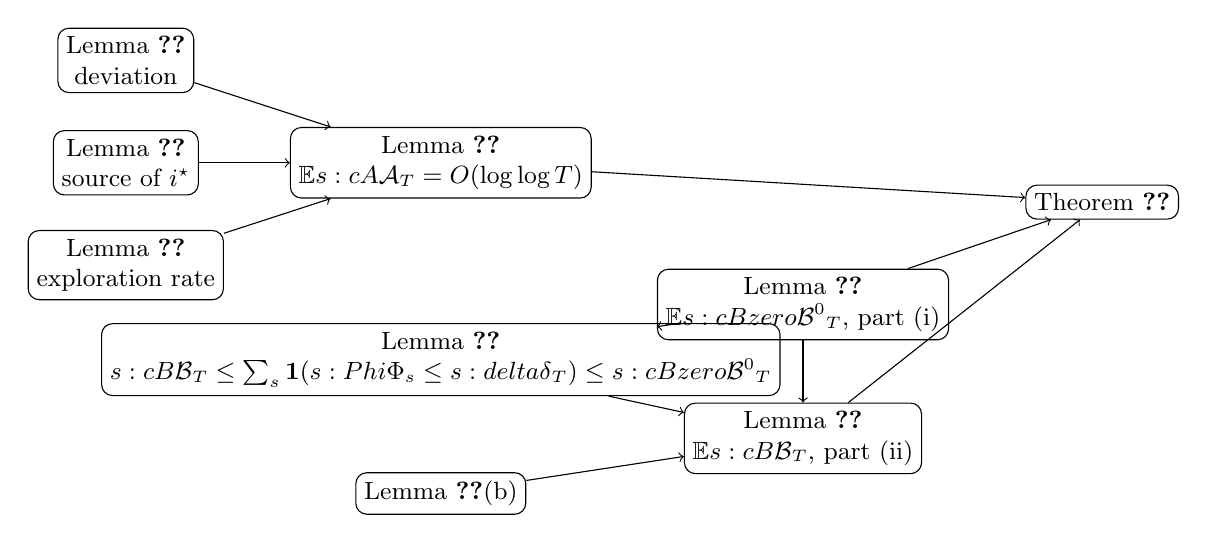
\begin{tikzpicture}[x=1cm,y=1cm,every node/.style={draw,rounded corners,font=\small,align=center,inner sep=3pt}]
  \node (dev) at (0,2.2) {Lemma~\ref{lem:deviation}\\deviation};
  \node (src) at (0,0.9) {Lemma~\ref{lem:source}\\source of $i^\star$};
  \node (del) at (0,-0.4) {Lemma~\ref{lem:delta}\\exploration rate};
  \node (opt) at (4,0.9) {Lemma~\ref{lem:optimal-arm}\\$\E\cA_T=O(\log\log T)$};
  \node (red) at (4,-1.6) {Lemma~\ref{lem:sub-reduction}\\$\cB_T\le\sum_s\ind(\Ph_s\le\dl_T)\le\cBz_T$};
  \node (kl) at (8.6,-0.9) {Lemma~\ref{lem:sub-kl}\\$\E\cBz_T$, part (i)};
  \node (cst) at (8.6,-2.6) {Lemma~\ref{lem:sub-constant}\\$\E\cB_T$, part (ii)};
  \node (D) at (4,-3.3) {Lemma~\ref{lem:D}(b)};
  \node (thm) at (12.4,0.4) {Theorem~\ref{thm:main}};
  \draw[->] (dev) -- (opt); \draw[->] (src) -- (opt); \draw[->] (del) -- (opt);
  \draw[->] (red) -- (kl); \draw[->] (red) -- (cst); \draw[->] (kl) -- (cst); \draw[->] (D) -- (cst);
  \draw[->] (opt) -- (thm); \draw[->] (kl) -- (thm); \draw[->] (cst) -- (thm);
\end{tikzpicture}
\end{center}

To prove Theorem~\ref{thm:main} we use the following decomposition.

\begin{lemma}[Decomposition]\label{lem:decomposition}
\uses{def:model, def:algo, def:proof-notation}
In the setting of Definition~\ref{def:proof-notation}, for every admissible $\varepsilon$ and every
$T\ge K$,
\begin{equation*}
\Nc_a(T)\le1+\underbrace{\sum_{t=K}^{T-1}\ind\big(\Ix_{i^\star}(t)<\mus-\varepsilon\big)}_{\cA_T}
+\underbrace{\sum_{t=K}^{T-1}\ind\big(\At_{t+1}=a,\ \Ix_a(t)\ge\mus-\varepsilon\big)}_{\cB_T}.
\end{equation*}
\end{lemma}

(See the proof in Subsection~\ref{sec:proof-lem-decomposition}.) This is the classical
decomposition of index policies; it is deterministic.

From this decomposition we use the following lemmas to control each term.

\begin{lemma}[The optimal arm]\label{lem:optimal-arm}
\uses{def:laws, def:ipm, def:model, def:algo, def:proof-notation, lem:source, lem:types}
In the setting of Definition~\ref{def:proof-notation}, let $\varepsilon$ be admissible, let $\Cone$
be the constant of Lemma~\ref{lem:source} for $p'=\nu'_{i^\star}$ and this $\etam$, and let
\begin{equation*}
\dt{s:Ctwo}\Ctwo:=\sum_{s\ge1}(s+1)^{|S|}\exp\big(-s\thet\kap_{\nu_{i^\star}}(\thet)\big)<\infty.
\end{equation*}
Then, for every $T\ge3$ and every sequence of source sizes,
\begin{equation*}
\E\cA_T\le\Cone\big(1+\Ctwo(1+\log\log T)\big).
\end{equation*}
\end{lemma}

(See the proof in Subsection~\ref{sec:optimal-arm}.) The target sample of $i^\star$ is handled as in
the classical proof of KL-UCB, with a deviation inequality under a $d$-constraint
(Lemma~\ref{lem:deviation}); the source sample is new: it is handled through an analysis law within
the margin $\etam$ and its exponential moment (Lemma~\ref{lem:source}), as \citet[Lemma~17]{PMRM26}
do for the mean gap.

\begin{lemma}[Reduction for the suboptimal arm]\label{lem:sub-reduction}
\uses{def:laws, def:ipm, def:model, def:constant, def:algo, def:proof-notation}
In the setting of Definition~\ref{def:proof-notation}, let $\varepsilon$ be admissible and, for
$s\ge1$,
\begin{equation*}
\dt{s:Phi}\Ph_s:=\min_{(q,q')\in\Pairs_a(\mus-\varepsilon)}\big[s\KL(\hnu_{a,s},q)+N'_a\KL(\hnu'_a,q')\big].
\end{equation*}
Then
\begin{equation*}
\cB_T\le\sum_{s=1}^{T}\ind(\Ph_s\le\dl_T)\le\dt{s:cBzero}\mathcal B^0_T
:=\sum_{s=1}^{T}\ind\big(s\,\Ks(\hnu_{a,s},\mus-\varepsilon)\le\dl_T\big).
\end{equation*}
\end{lemma}

(See the proof in Subsection~\ref{sec:suboptimal-arm}.) Classical: the counting over the values of
$\Nc_a(t)$ of index policies; no contribution here. The first inequality serves part~(ii) of
Theorem~\ref{thm:main} (Lemma~\ref{lem:sub-constant}); the second serves part~(i)
(Lemma~\ref{lem:sub-kl}).

\begin{lemma}[The KL-UCB term]\label{lem:sub-kl}
\uses{def:laws, def:model, def:proof-notation, lem:types}
In the setting of Definition~\ref{def:proof-notation}, let $\varepsilon$ be admissible and
$\dt{s:Ke}\mathcal K_\varepsilon:=\Ks(\nu_a,\mus-\varepsilon)$. Then $\Ke\in(0,\infty)$, and for
every $\xi\in(0,\Ke)$ there is $\varrho_\xi>0$ such that, for every $T\ge3$,
\begin{equation*}
\E\cBz_T\le\frac{\dl_T}{\Ke-\xi}+\Cthree,\qquad
\dt{s:Cthree}\Cthree:=\sum_{s\ge1}(s+1)^{|S|}e^{-s\kap_{\nu_a}(\varrho_\xi)}<\infty.
\end{equation*}
\end{lemma}

(See the proof in Subsection~\ref{sec:proof-lem-sub-kl}.) As in the classical proof of KL-UCB
\citep{CGMMS13}, with the method of types in place of their deviation inequalities; no
contribution here.

\begin{lemma}[The constant term]\label{lem:sub-constant}
\uses{def:laws, def:ipm, def:model, def:constant, def:algo, def:proof-notation}
In the setting of Definition~\ref{def:proof-notation}, assume $\mus<\xmax$ and
$N'_a(T)/\log T\to c_a\in(0,\infty)$, and let $D:=\Dc_a(c_a)$ and $\gamma>0$. There is $\varrho_0>0$
such that, for every admissible $\varepsilon$ with $\varepsilon<\varrho_0$, the quantity $\cB_T$ of
this $\varepsilon$ satisfies
\begin{equation*}
\E\cB_T\le(D+\gamma)\log T+o(\log T).
\end{equation*}
\end{lemma}

(See the proof in Subsection~\ref{sec:proof-lem-sub-constant}.) This lemma is new: it is the only
place where the source sample of the suboptimal arm enters, through the margin of
Lemma~\ref{lem:D}(b) and a lower-semicontinuity argument.

From these lemmas the proof of the theorem is short.

\begin{proof}[Proof of Theorem~\ref{thm:main}]
\proves{thm:main}
\uses{def:laws, def:ipm, def:model, def:constant, def:algo, def:proof-notation, lem:decomposition, lem:optimal-arm, lem:sub-reduction, lem:sub-kl, lem:sub-constant, lem:lsc, lem:D}
\emph{Part~(i).} Let $\varepsilon$ be admissible and $\xi\in(0,\Ke)$. Taking expectations in
Lemma~\ref{lem:decomposition} (\emph{the decomposition}), then using Lemma~\ref{lem:optimal-arm}
(\emph{the optimal arm}), Lemma~\ref{lem:sub-reduction} (\emph{the reduction}) and
Lemma~\ref{lem:sub-kl} (\emph{the KL-UCB term}), we get
\begin{align*}
\E \Nc_a(T)&\le1+\E\cA_T+\E\cB_T\\
&\le1+\Cone\big(1+\Ctwo(1+\log\log T)\big)+\E\cBz_T\\
&\le1+\Cone\big(1+\Ctwo(1+\log\log T)\big)+\frac{\dl_T}{\Ke-\xi}+\Cthree .
\end{align*}
As $\dl_T/\log T\to1$, this gives
\begin{equation*}
\limsup_{T\to\infty}\frac{\E \Nc_a(T)}{\log T}\le\frac{1}{\Ke-\xi}.
\end{equation*}
Let $\xi\to0$, then $\varepsilon\to0$. The function $\ell\mapsto\Ks(\nu_a,\ell)$ is lower
semicontinuous (Lemma~\ref{lem:lsc}(b) with parameter $\ell$ and the closed set
$\{(\ell,q):\mean(q)\ge\ell\}$), so $\liminf_{\varepsilon\to0}\Ke\ge\Ks(\nu_a,\mus)$. This holds
also when $\Ks(\nu_a,\mus)=\infty$.

\emph{Part~(ii).} If $\mus=\xmax$, then $\Dc_a(c_a)=0$ (Lemma~\ref{lem:D}) and
$\Ks(\nu_a,\mus)=\infty$, so~(i) gives~(ii). Let $\mus<\xmax$. We split according to
$c_a$.
\begin{itemize}
\item If $c_a=0$: $\Jf_a(x,0)=x\Ko$ (take $q'=q$), so $\Dc_a(0)=1/\Ko$ and~(i) gives~(ii).
\item If $c_a>0$: fix $\gamma>0$ and take $\varrho_0$ from Lemma~\ref{lem:sub-constant}. We choose
  \begin{equation*}
  \varepsilon:=\min(\varrho_0,1,\gap_a)/2,
  \end{equation*}
  which is admissible and below $\varrho_0$, so that Lemma~\ref{lem:sub-constant} applies.
  Lemmas~\ref{lem:decomposition}, \ref{lem:optimal-arm} and~\ref{lem:sub-constant} give
  \begin{equation*}
  \E \Nc_a(T)\le1+O(\log\log T)+(D+\gamma)\log T+o(\log T),
  \end{equation*}
  so $\limsup_T\E \Nc_a(T)/\log T\le \Dc_a(c_a)+\gamma$ for every $\gamma>0$.\qedhere
\end{itemize}
\end{proof}

\begin{proof}[Proof of Corollary~\ref{cor:optimal}]
\proves{cor:optimal}
\uses{def:class, def:constant, def:algo, thm:main, prop:lower}
On $\Thet$ every arm satisfies the drift condition, in particular an optimal arm, so
Theorem~\ref{thm:main}(i) applies for every sequence $N'$: every suboptimal arm has
$\E \Nc_k(T)=O(\log T)=o(T^\alpha)$, since $\Ks(\nu_k,\mus)>0$. So \Alg{} lies in $\Cons(N')$.
Proposition~\ref{prop:lower} (\emph{the lower bound}, with $\cbar_a=c_a$) and
Theorem~\ref{thm:main}(ii) give
\begin{equation*}
\Dc_a(c_a)\le\liminf_{T\to\infty}\frac{\E \Nc_a(T)}{\log T}\le\limsup_{T\to\infty}\frac{\E \Nc_a(T)}{\log T}\le \Dc_a(c_a).
\end{equation*}
The regret is $\Reg_T=\sum_a(\mus-\mk_a)\E \Nc_a(T)$, which gives the last two claims.
\end{proof}

\subsection{Concentration on a finite support}\label{sec:concentration}

The bound of Lemma~\ref{lem:optimal-arm} rests on three concentration facts, stated here and proved
in the subsections that follow.

\begin{lemma}[Deviation under a $d$-constraint]\label{lem:deviation}
\uses{def:laws, def:ipm, lem:ipm, lem:lsc}
Let $p\in\Simp$, $\varepsilon,\varrho\in(0,1]$, $\theta:=\min(\varepsilon,\varrho)$, and
\begin{equation*}
\dt{s:H}\Hr_\varrho(r):=\min\{\KL(r,q):q\in\Simp,\ \mean(q)\ge \mean(p)-\varepsilon,\ d(q,p)\le\varrho\}
\end{equation*}
(a minimum: the set contains $p$ and is compact, as $m$ and $d$ are continuous,
Lemma~\ref{lem:ipm}(d), and $\KL(r,\cdot)$ is lower semicontinuous, Lemma~\ref{lem:lsc}). Let
$\hat p_n$ be the empirical law of $n\ge1$ i.i.d.\ draws from $p$. Then, for every $u\ge0$,
\begin{equation*}
\PP(n\Hr_\varrho(\hat p_n)>u)\le(n+1)^{|S|}\exp(-u-n\theta\kap_p(\theta)).
\end{equation*}
\end{lemma}

(See the proof in Subsection~\ref{sec:proof-lem-deviation}.) \emph{Role.} The target sample of the
optimal arm in Lemma~\ref{lem:optimal-arm}, with $p=\nu_{i^\star}$ and $\varrho=\etam/2$.

\begin{lemma}[Exponential moment of the source of the optimal arm]\label{lem:source}
\uses{def:laws, def:ipm}
Let $p'\in\Simp$, $\eta\in(0,1]$, $n\ge0$, and let $\hat p'$ be the empirical law of $n$ i.i.d.\
draws from $p'$. Let $\dt{s:qbar}\qbar':=p'$ if $n=0$; $\qbar':=\hat p'$ if $n\ge1$ and
$d(\hat p',p')\le\eta/2$; and $\qbar':=(1-\frac\eta2)p'+\frac\eta2\hat p'$ otherwise. Let
$\dt{s:Lambda}\Lam:=n\KL(\hat p',\qbar')$ ($\Lam:=0$ if $n=0$). Then $d(\qbar',p')\le\eta/2$ and
\begin{equation*}
\E e^{\Lam}\le\dt{s:Cone}\Cone:=1+\sup_{n'\ge0}(n'+1)^{|S|}\exp\Big(-n'\frac\eta2\kap_{p'}\Big(\frac\eta2\Big)\Big)<\infty .
\end{equation*}
\end{lemma}

(See the proof in Subsection~\ref{sec:proof-lem-source}.) \emph{Role.} The source sample of the
optimal arm in Lemma~\ref{lem:optimal-arm}, with $p'=\nu'_{i^\star}$ and $n=N'_{i^\star}$: the bound
does not depend on $n$.

\begin{lemma}[The exploration rate]\label{lem:delta}
\uses{def:algo}
For $\dl_t$ as in Definition~\ref{def:algo} and every $T\ge3$,
\begin{equation*}
\sum_{t=1}^{T-1}e^{-\dl_t}\le1+\log\log T,
\end{equation*}
and for every $z\ge0$, $|\{t\ge1:\dl_t\le z\}|\le e^z$.
\end{lemma}

(See the proof in Subsection~\ref{sec:proof-lem-delta}.) \emph{Role.} The sum over the rounds in
Lemma~\ref{lem:optimal-arm}.

\subsection{Proof of Lemma~\ref{lem:decomposition}}\label{sec:proof-lem-decomposition}

\begin{proof}
\proves{lem:decomposition}
\uses{def:model, def:algo, def:proof-notation}
Arm $a$ is pulled once in the first $K$ rounds, so
\begin{equation*}
\Nc_a(T)=1+\sum_{t=K}^{T-1}\ind(\At_{t+1}=a).
\end{equation*}
If $\At_{t+1}=a$ then $\Ix_a(t)\ge \Ix_{i^\star}(t)$, so $\Ix_{i^\star}(t)<\mus-\varepsilon$ or
$\Ix_a(t)\ge\mus-\varepsilon$. So we split according to the event
$\{\Ix_{i^\star}(t)<\mus-\varepsilon\}$:
\begin{align*}
\ind(\At_{t+1}=a)&\le\ind\big(\Ix_{i^\star}(t)<\mus-\varepsilon\big)
+\ind\big(\At_{t+1}=a,\ \Ix_{i^\star}(t)\ge\mus-\varepsilon\big)\\
&\le\ind\big(\Ix_{i^\star}(t)<\mus-\varepsilon\big)
+\ind\big(\At_{t+1}=a,\ \Ix_a(t)\ge\mus-\varepsilon\big) && (\Ix_a(t)\ge \Ix_{i^\star}(t)).
\end{align*}
Summing over $t\in\{K,\dots,T-1\}$ gives the claim.
\end{proof}

\subsection{Proof of Lemma~\ref{lem:optimal-arm}}\label{sec:optimal-arm}

\begin{proof}
\proves{lem:optimal-arm}
\uses{def:laws, def:ipm, def:model, def:algo, def:proof-notation, lem:ipm, lem:lsc, lem:source, lem:deviation, lem:delta}
\emph{Idea.} If the index of $i^\star$ is below $\mus-\varepsilon$, no pair $(q,\qbar')$ with
$q$ near $\nu_{i^\star}$ fits in the budget $\dl_t$. Either the source cost $\Lam$ alone
exceeds $\dl_t$, which happens at most $e^\Lam$ times, or the target sample deviates, which
Lemma~\ref{lem:deviation} makes rare; the factor $e^\Lam$ is integrated by Lemma~\ref{lem:source}.

\emph{Setting.} Write $p:=\nu_{i^\star}$ and $p':=\nu'_{i^\star}$, and let $\qbar'$ and $\Lam$ be
those of Lemma~\ref{lem:source} for the source sample of arm $i^\star$, with the parameter $\eta$ of
Lemma~\ref{lem:source} equal to the margin $\etam$ of Definition~\ref{def:proof-notation}: they are
functions of that sample. \emph{Goal.}
$\E[\cA_T\mid\text{source}]\le e^\Lam+e^\Lam\Ctwo(1+\log\log T)$.

\emph{Step 1 (feasible pairs).} Let $q\in\Simp$ with $\mean(q)\ge\mus-\varepsilon$ and
$d(q,p)\le\etam/2$. Then
\begin{align*}
d(q,\qbar')&\le d(q,p)+d(p,p')+d(p',\qbar') && \text{(Lemma~\ref{lem:ipm}(a))}\\
&\le\frac\etam2+(L_{i^\star}-\etam)+\frac\etam2=L_{i^\star} && \text{(as $d(p,p')\le L_{i^\star}-\etam$, Lemma~\ref{lem:source})}.
\end{align*}
So if $\Nc_{i^\star}(t)\KL(\hnu_{i^\star}(t),q)+\Lam\le\dl_t$, the pair $(q,\qbar')$ is
feasible in the index of $i^\star$, and $\Ix_{i^\star}(t)\ge \mean(q)\ge\mus-\varepsilon$.

\emph{Step 2 (the event to control).} Let $\Hr_{\etam/2}$ be as in Lemma~\ref{lem:deviation} for this
$p$, $\varepsilon$ and $\varrho=\etam/2$ (so $\mean(p)=\mus$), and take $q$ a minimiser in
$\Hr_{\etam/2}(\hnu_{i^\star}(t))$ (the feasible set contains $p$ and is compact, and $\KL$ is lower
semicontinuous, Lemma~\ref{lem:lsc}). By contraposition of Step~1, and since
$\Nc_{i^\star}(t)\in\{1,\dots,t\}$ for $t\ge K$,
\begin{align*}
\{\Ix_{i^\star}(t)<\mus-\varepsilon\}
&\subset\{\Nc_{i^\star}(t)\Hr_{\etam/2}(\hnu_{i^\star}(t))>\dl_t-\Lam\}\\
&\subset\{\dl_t\le\Lam\}\cup\bigcup_{s=1}^{t}\{s\Hr_{\etam/2}(\hnu_{i^\star,s})>\dl_t-\Lam>0\}.
\end{align*}

\emph{Step 3 (summing).} By Lemma~\ref{lem:delta} (\emph{the exploration rate}), at most $e^\Lam$
rounds have $\dl_t\le\Lam$. The stack of $i^\star$ is independent of its source sample, so,
conditionally on the source sample, Lemma~\ref{lem:deviation} applies with $u=\dl_t-\Lam$:
\begin{equation*}
\sum_{s=1}^t\PP\big(s\Hr_{\etam/2}(\hnu_{i^\star,s})>\dl_t-\Lam\ \big|\ \text{source}\big)\le e^{\Lam-\dl_t}\Ctwo .
\end{equation*}
Summing over $t$ with Lemma~\ref{lem:delta} gives the goal,
\begin{equation*}
\E[\cA_T\mid\text{source}]\le e^\Lam+e^\Lam\Ctwo(1+\log\log T).
\end{equation*}
Take expectations and use $\E e^\Lam\le\Cone$ (Lemma~\ref{lem:source}, which holds for every
$N'_{i^\star}$).
\end{proof}

\subsection{Proof of Lemma~\ref{lem:sub-reduction}}\label{sec:suboptimal-arm}

\begin{proof}
\proves{lem:sub-reduction}
\uses{def:laws, def:ipm, def:model, def:constant, def:algo, def:proof-notation, lem:index, lem:ipm, lem:lsc}
\emph{Step 1 (the minimum exists).} $\Pairs_a(\mus-\varepsilon)$ is closed in the compact
$\Simp^2$ ($m$ and $d$ are continuous, Lemma~\ref{lem:ipm}(d)) and contains $(\dirac,\dirac)$, since
$\mus-\varepsilon<\mus\le\xmax$; the objective is lower semicontinuous with values in
$[0,\infty]$ (Lemma~\ref{lem:lsc}(a)).

\emph{Step 2 (a high index gives a small $\Phi$).} If $\At_{t+1}=a$, $\Ix_a(t)\ge\mus-\varepsilon$
and $\Nc_a(t)=s$, the maximum defining $\Ix_a(t)$ is attained (Lemma~\ref{lem:index}) at a pair in
$\Pairs_a(\mus-\varepsilon)$ whose objective is at most $\dl_t\le\dl_T$; so
$\Ph_s\le\dl_T$.

\emph{Step 3 (counting).} Since $\Nc_a$ increases at each pull of $a$, for each $s$ at most one $t$
has $\At_{t+1}=a$ and $\Nc_a(t)=s$. So, splitting according to the value $s$ of $\Nc_a(t)$,
\begin{align*}
\cB_T&\le\sum_{s=1}^{T}\ind(\Ph_s\le\dl_T)\sum_t\ind(\At_{t+1}=a,\Nc_a(t)=s) && \text{(Step~2)}\\
&\le\sum_{s=1}^{T}\ind(\Ph_s\le\dl_T) && \text{(at most one $t$ for each $s$)}.
\end{align*}
Finally $\Ph_s\ge s\,\Ks(\hnu_{a,s},\mus-\varepsilon)$: drop the nonnegative source term and
the constraint on $d$.
\end{proof}

\subsection{Proof of Lemma~\ref{lem:sub-kl}}\label{sec:proof-lem-sub-kl}

\begin{proof}
\proves{lem:sub-kl}
\uses{def:laws, def:model, def:proof-notation, lem:projection, lem:lsc, lem:types}
$\mk_a<\mus-\varepsilon<\xmax$, so $\Ke\in(0,\infty)$ by Lemma~\ref{lem:projection}. The
function $r\mapsto\Ks(r,\mus-\varepsilon)$ is lower semicontinuous (Lemma~\ref{lem:lsc}(b) with
$h(r,q):=\KL(r,q)$ plus the indicator, $0$ or $\infty$, of the closed set
$\{\mean(q)\ge\mus-\varepsilon\}$), so there is $\varrho_\xi>0$ with
\begin{equation*}
\Ks(r,\mus-\varepsilon)>\Ke-\xi\qquad\text{whenever }\TV(r,\nu_a)<\varrho_\xi .
\end{equation*}
For $s>\dl_T/(\Ke-\xi)$, the event $s\Ks(\hnu_{a,s},\mus-\varepsilon)\le\dl_T$ implies
$\TV(\hnu_{a,s},\nu_a)\ge\varrho_\xi$, of probability at most
$(s+1)^{|S|}e^{-s\kap_{\nu_a}(\varrho_\xi)}$ (Lemma~\ref{lem:types}(c)). The other indices $s$
contribute at most $\dl_T/(\Ke-\xi)$.
\end{proof}

\subsection{Proof of Lemma~\ref{lem:sub-constant}}\label{sec:proof-lem-sub-constant}

\begin{proof}
\proves{lem:sub-constant}
\uses{def:laws, def:ipm, def:model, def:constant, def:algo, def:proof-notation, lem:lsc, lem:D, lem:types, lem:sub-reduction, lem:sub-kl}
\emph{Idea.} After $(D+\gamma)\log T$ pulls of $a$, the minimum $\Ph_s$ is, up to the factor
$\log T$, a lower semicontinuous function of the empirical laws, of the source rate and of the level,
which exceeds $1$ with a margin at the true values (Lemma~\ref{lem:D}(b)). By semicontinuity it still
exceeds $\dl_T/\log T$ near them, and the empirical laws are near the true laws except on rare
events.

\emph{Step 1 (a lower semicontinuous function).} On $\Simp\times\Simp\times[0,\infty)\times\mathbb R$
let
\begin{equation*}
\dt{s:psi}\psif(r,r',\beta,\mu):=\min_{(q,q')\in\Pairs_a(\mu)}\big[(D+\gamma)\KL(r,q)+\beta\KL(r',q')\big].
\end{equation*}
The integrand plus the indicator of the closed set
$\{(q,q',\mu):\mean(q)\ge\mu,\ d(q,q')\le L_a\}$ is lower semicontinuous (Lemma~\ref{lem:lsc}(a)), so
$\psif$ is lower semicontinuous (Lemma~\ref{lem:lsc}(b)). By Lemma~\ref{lem:D}(b) (\emph{the margin
above the constant}),
\begin{equation*}
\psif(\nu_a,\nu'_a,c_a,\mus)=\Jf_a(D+\gamma,c_a)\ge1+\gamma\Ko>1+\gamma\Ko/2.
\end{equation*}
So there is $\varrho_0\in(0,c_a)$ such that $\psif(r,r',\beta,\mu)>1+\gamma\Ko/2$ whenever
\begin{equation*}
\TV(r,\nu_a)<\varrho_0,\qquad\TV(r',\nu'_a)<\varrho_0,\qquad|\beta-c_a|<\varrho_0,\qquad
|\mu-\mus|<\varrho_0 .
\end{equation*}

\emph{Step 2 (homogeneity).} Fix $\varepsilon$ as in the statement, and let $T_0$ be such that, for
$T\ge T_0$, $|N'_a(T)/\log T-c_a|<\varrho_0$ and $\dl_T\le(1+\gamma\Ko/2)\log T$. Let
$s_1:=\lceil(D+\gamma)\log T\rceil$. For $s\ge s_1$, $s\KL\ge(D+\gamma)\log T\,\KL$, so
\begin{equation*}
\Ph_s\ \ge\ \log T\cdot\psif\Big(\hnu_{a,s},\hnu'_a,\frac{N'_a(T)}{\log T},\mus-\varepsilon\Big).
\end{equation*}

\emph{Step 3 (splitting on the source of $a$).} Let $\cE':=\{\TV(\hnu'_a,\nu'_a)<\varrho_0\}$ and
$\cE_s:=\{\TV(\hnu_{a,s},\nu_a)<\varrho_0\}$. For $T\ge T_0$, on $\cE'\cap\cE_s$ with $s\ge s_1$,
Steps~1 and~2 give
\begin{equation*}
\Ph_s>(1+\gamma\Ko/2)\log T\ge\dl_T .
\end{equation*}
So, by Lemma~\ref{lem:sub-reduction} (\emph{the reduction}), splitting on $\cE'$,
\begin{equation*}
\cB_T\le\ind_{\cE'}\Big(s_1-1+\sum_{s\ge1}\ind(\cE_s^c)\Big)+\ind_{\cE'^c}\,\cBz_T .
\end{equation*}

\emph{Step 4 (expectations).} $\cE'$ depends on the source sample of $a$ and $\cBz_T$ on its stack,
which are independent, so, by Lemma~\ref{lem:types}(c),
\begin{equation*}
\E\cB_T\le(D+\gamma)\log T+\sum_{s\ge1}(s+1)^{|S|}e^{-s\kap_{\nu_a}(\varrho_0)}+\PP(\cE'^c)\,\E\cBz_T .
\end{equation*}
Finally $\PP(\cE'^c)\le(N'_a+1)^{|S|}e^{-N'_a\kap_{\nu'_a}(\varrho_0)}\to0$ because
$N'_a(T)\to\infty$ ($c_a>0$), and $\E\cBz_T=O(\log T)$ by Lemma~\ref{lem:sub-kl}.
\end{proof}

\subsection{Proof of Lemma~\ref{lem:deviation}}\label{sec:proof-lem-deviation}

\begin{proof}
\proves{lem:deviation}
\uses{def:laws, def:ipm, lem:ipm, lem:lsc, lem:types}
\emph{Idea.} A type $r$ with $n\Hr_\varrho(r)>u$ is infeasible, hence far from $p$; mixing it with $p$
gives a feasible law, and convexity turns the distance into a gain $\theta\KL(r,p)$.

\emph{Step 1 (infeasible types are far from $p$).} Let $r\in\Tn_n$ with $n\Hr_\varrho(r)>u\ge0$.
Then $\Hr_\varrho(r)>0$, so $r$ is not feasible ($q=r$ would give $0$). We split according to the
constraint that $r$ violates:
\begin{itemize}
\item either $\mean(r)<\mean(p)-\varepsilon$, and then $\TV(r,p)\ge|\mean(r)-\mean(p)|>\varepsilon\ge\theta$
  (Lemma~\ref{lem:ipm}(c));
\item or $d(r,p)>\varrho$, and then $\TV(r,p)\ge d(r,p)>\varrho\ge\theta$.
\end{itemize}
So $\KL(r,p)\ge\kap_p(\theta)$.

\emph{Step 2 (a feasible mixture).} Let $q_\theta:=(1-\theta)p+\theta r$. Then
$\mean(q_\theta)\ge(1-\theta)\mean(p)\ge \mean(p)-\theta\ge \mean(p)-\varepsilon$ (as $0\le m\le1$), and
$d(q_\theta,p)=\theta\,d(r,p)\le\theta\le\varrho$ (Lemma~\ref{lem:ipm}(b,c)). By convexity of
$\KL(r,\cdot)$,
\begin{equation*}
\Hr_\varrho(r)\le\KL(r,q_\theta)\le(1-\theta)\KL(r,p).
\end{equation*}

\emph{Step 3 (conclusion).} Steps~1 and~2 give
\begin{equation*}
\KL(r,p)\ge \Hr_\varrho(r)+\theta\KL(r,p)\ge \Hr_\varrho(r)+\theta\kap_p(\theta).
\end{equation*}
So, by Lemma~\ref{lem:types}(b),
\begin{equation*}
\PP(\hat p_n=r)\le e^{-n\Hr_\varrho(r)-n\theta\kap_p(\theta)}<e^{-u-n\theta\kap_p(\theta)}
\end{equation*}
(both sides are $0$ if $\KL(r,p)=\infty$). Sum over the at most $(n+1)^{|S|}$ types.
\end{proof}

\subsection{Proof of Lemma~\ref{lem:source}}\label{sec:proof-lem-source}

\begin{proof}
\proves{lem:source}
\uses{def:laws, def:ipm, lem:ipm, lem:types}
The bound on $d(\qbar',p')$ follows from Lemma~\ref{lem:ipm}(b,c) in the third case. Let $n\ge1$
and $\cE:=\{d(\hat p',p')\le\eta/2\}$. We split according to $\cE$.
\begin{itemize}
\item On $\cE$, $\Lam=0$, so $\E[e^\Lam\ind_{\cE}]\le1$.
\item On $\cE^c$, convexity gives $\Lam\le(1-\frac\eta2)\,n\KL(\hat p',p')$, and every type $r'$
  with $d(r',p')>\eta/2$ has $\TV(r',p')>\eta/2$, hence $\KL(r',p')\ge\kap_{p'}(\eta/2)$. By
  Lemma~\ref{lem:types},
  \begin{equation*}
  \E[e^\Lam\ind_{\cE^c}]\le\sum_{r'}e^{-n\KL(r',p')}e^{(1-\frac\eta2)n\KL(r',p')}
  =\sum_{r'}e^{-\frac\eta2n\KL(r',p')}\le(n+1)^{|S|}e^{-n\frac\eta2\kap_{p'}(\eta/2)},
  \end{equation*}
  the sums running over the types with $d(r',p')>\eta/2$ and $\KL(r',p')<\infty$ (the others have
  probability $0$).
\end{itemize}
The supremum is finite because $\kap_{p'}(\eta/2)>0$ (Lemma~\ref{lem:types}(c)).
\end{proof}

\subsection{Proof of Lemma~\ref{lem:delta}}\label{sec:proof-lem-delta}

\begin{proof}
\proves{lem:delta}
\uses{def:algo}
For $t\le3$, $e^{-\dl_t}=1/(3\log3)\le0.31$. For $t\ge4$,
\begin{equation*}
e^{-\dl_t}=\frac1{t\log t}\le\int_{t-1}^{t}\frac{du}{u\log u}.
\end{equation*}
Hence
\begin{equation*}
\sum_{t=1}^{T-1}e^{-\dl_t}\le0.93+\int_3^T\frac{du}{u\log u}=0.93+\log\log T-\log\log3\le1+\log\log T,
\end{equation*}
since $\log\log3>0.09$. Finally $\dl_t\ge\log t$, so $\dl_t\le z$ implies $t\le e^z$.
\end{proof}

% ----------------------------------------------------------------
\section{\texorpdfstring{Proof of Proposition~\ref{prop:lower}}{Proof of Proposition 4.2}}\label{sec:proof-lower}

In this appendix we prove Proposition~\ref{prop:lower}. The proof follows
\citet[Appendix~A]{PMM25}, with the source samples written as forced pulls so that the change of
measure of Lemma~\ref{cite:GMS19-6} applies as stated.

\paragraph{Relation with the class of \texorpdfstring{\citet{PMRM26}}{Prevost et al. (2026)}} The
class $\mathcal C_L$ of \citet[Section~4.2]{PMRM26} asks for consistency on every pair of laws on
$[0,1]$ with mean drift at most $L_k$ and for every source strategy. When $d$ has \propM{}, every
instance of $\Thet$ is such a pair, and deterministic sizes are a source strategy, so
$\mathcal C_L\subset\Cons(N')$: Proposition~\ref{prop:lower} applies to every learner of
$\mathcal C_L$.

\paragraph{A lower bound on the Bernoulli divergence} The proof uses the following inequality,
derived from Lemma~\ref{cite:GMS19-11}.

\begin{lemma}[A lower bound on $\kl$]\label{lem:kl-lower}
For all $p,\tilde p\in[0,1]$,
\begin{equation*}
\kl(p,\tilde p)\ge p\log\frac1{\tilde p}-\log2.
\end{equation*}
\end{lemma}

(See the proof in Subsection~\ref{sec:proof-lem-kl-lower}.) \emph{Role.} Step~2 of the proof of
Proposition~\ref{prop:lower}, with $p=1-\E \Nc_a(T)/T$. It is a direct consequence of
Lemma~\ref{cite:GMS19-11}, not printed in this form in \citet{GMS19}.

\begin{proof}[Proof of Proposition~\ref{prop:lower}]
\proves{prop:lower}
\uses{def:laws, def:ipm, def:model, def:class, def:constant, cite:GMS19-6, lem:kl-lower, lem:D}
\emph{Idea.} An alternative pair $(q,q')$ of~\eqref{eq:sup-form} gives an instance of $\Thet$ in
which $a$ is optimal. A consistent learner distinguishes the two instances, and the information it
needs is shared between the source samples, which are forced, and the pulls of $a$.

\emph{Setting.} Fix $\alpha\in(0,1)$ and a pair $(q,q')\in\Simp^2$ with $\mean(q)>\mus$,
$d(q,q')<L_a$ and finite $\KL(\nu_a,q)$, $\KL(\nu'_a,q')$. Let $(\tilde\nu,\tilde\nu')$ be
$(\nu,\nu')$ with $(\nu_a,\nu'_a)$ replaced by $(q,q')$: it lies in $\Thet$, and $a$ is its only
optimal arm. Write $\tilde\E$ for the expectations on $(\tilde\nu,\tilde\nu')$. \emph{Goal.}
\begin{equation*}
\liminf_{T\to\infty}\frac{\E \Nc_a(T)}{\log T}\ge\frac{1-\alpha-\cbar_a\KL(\nu'_a,q')}{\KL(\nu_a,q)}.
\end{equation*}

\emph{Step 1 (the source as forced pulls).} Fix $T$. Consider the bandit with $2K$ arms whose arm
$(k,\mathrm{src})$ has law $\nu'_k$ and arm $(k,\mathrm{tgt})$ has law $\nu_k$, and the strategy that
first pulls each arm $(k,\mathrm{src})$ exactly $N'_k(T)$ times, then plays $\pi$ for $T$ rounds on
the arms $(k,\mathrm{tgt})$, feeding it the first observations as source samples. The joint law of
(source samples, randomisation, online observations) is the same as in the transfer game, and the
counts at the final round are $N'_k(T)$ for $(k,\mathrm{src})$ and $\Nc_k(T)$ for $(k,\mathrm{tgt})$.
The same holds for $(\tilde\nu,\tilde\nu')$, with the same strategy.

\emph{Step 2 (change of measure).} Apply Lemma~\ref{cite:GMS19-6} to these two $2K$-armed instances,
which differ only at $(a,\mathrm{src})$ and $(a,\mathrm{tgt})$, with $Z:=1-\Nc_a(T)/T$. The $2K$-armed
game has horizon $T+\sum_kN'_k(T)$ (not $T$), and $Z$ is measurable with respect to its history up to
that horizon, which is what Lemma~\ref{cite:GMS19-6} asks for that game; the counts there are
$N'_k(T)$ at $(k,\mathrm{src})$ and $\Nc_k(T)$ at $(k,\mathrm{tgt})$. Let $p_T:=1-\E \Nc_a(T)/T$ and
$\tilde p_T:=1-\tilde\E \Nc_a(T)/T$. Then
\begin{align*}
N'_a(T)\KL(\nu'_a,q')+\E \Nc_a(T)\,\KL(\nu_a,q)
&\ge\kl(p_T,\tilde p_T) && \text{(Lemma~\ref{cite:GMS19-6})}\\
&\ge\Big(1-\frac{\E \Nc_a(T)}{T}\Big)\log\frac{T}{T-\tilde\E \Nc_a(T)}-\log2 && \text{(Lemma~\ref{lem:kl-lower})}.
\end{align*}

\emph{Step 3 (consistency).} Since $\pi\in\Cons(N')$ and $a$ is suboptimal for $(\nu,\nu')$,
$\E \Nc_a(T)=o(T^\alpha)$, so $\E \Nc_a(T)/T\to0$. Every $k\ne a$ is suboptimal for
$(\tilde\nu,\tilde\nu')\in\Thet$, so $T-\tilde\E \Nc_a(T)=\sum_{k\ne a}\tilde\E \Nc_k(T)\le T^\alpha$ for
$T$ large, and
\begin{equation*}
\log\frac{T}{T-\tilde\E \Nc_a(T)}\ge(1-\alpha)\log T .
\end{equation*}

\emph{Step 4 (conclusion).} Dividing by $\log T$ and taking the $\liminf$,
\begin{equation*}
\liminf_{T\to\infty}\frac{\E \Nc_a(T)\KL(\nu_a,q)}{\log T}\ge(1-\alpha)-\cbar_a\KL(\nu'_a,q').
\end{equation*}
As $\E \Nc_a(T)\ge0$ and $\alpha$ is arbitrary,
\begin{equation*}
\liminf_{T\to\infty}\frac{\E \Nc_a(T)}{\log T}\ge\frac{(1-\cbar_a\KL(\nu'_a,q'))_+}{\KL(\nu_a,q)}.
\end{equation*}
Taking the supremum over the pairs gives $\Dc_a(\cbar_a)$ by Lemma~\ref{lem:D}(a) (\emph{the constant
as a supremum}) if $\mus<\xmax$; if $\mus=\xmax$, $\Dc_a(\cbar_a)=0$ and there is nothing to
prove.
\end{proof}

\subsection{Proof of Lemma~\ref{lem:kl-lower}}\label{sec:proof-lem-kl-lower}

\begin{proof}
\proves{lem:kl-lower}
\uses{cite:GMS19-11}
By Lemma~\ref{cite:GMS19-11},
\begin{equation*}
\kl(p,\tilde p)=p\log\frac1{\tilde p}+(1-p)\log\frac1{1-\tilde p}+\big(p\log p+(1-p)\log(1-p)\big).
\end{equation*}
The second term is nonnegative, since $1-p\ge0$ and $1-\tilde p\in[0,1]$. The last term is at least
$-\log2$ (Lemma~\ref{cite:GMS19-11}). Dropping the second term gives the claim (both sides are
$+\infty$ when $p>0=\tilde p$).
\end{proof}

% ----------------------------------------------------------------
\section{Proofs of the structure results}\label{sec:proof-structure}

In this appendix, as in Section~\ref{sec:structure}, $L\in(0,\infty)^K$,
$(\nu,\nu')\in\Simp^K\times\Simp^K$ (no drift condition), $a$ is an arm with $\mk_a<\mus<\xmax$,
and $\Jf^d$, $\Dc^d$, $\Pairs^d_a$ are $\Jf_a$, $\Dc_a$, $\Pairs_a$ for the pseudo-distance $d$; the
hypothesis $\mean(\nu'_a)\le\mus+L_a$ is used only where it is stated. As
$\mus-L_a<\mus<\xmax$, $\Qs$ and $\Qps$ are well defined (Lemma~\ref{lem:projection}):
$\mean(\Qs)=\mus$, and $\mean(\Qps)=\mus-L_a$ if $\Kop>0$, while $\Qps=\nu'_a$ if $\Kop=0$.
The tool for the criteria is the following lemma; the propositions follow, one subsection each, in
the order of Section~\ref{sec:structure}.

\begin{lemma}[Criterion at a point]\label{lem:criterion-point}
\uses{def:ipm, def:constant}
Let $L\in(0,\infty)^K$, $(\nu,\nu')\in\Simp^K\times\Simp^K$, let $a$ be an arm with
$\mk_a<\mus<\xmax$, let $d$ be a pseudo-distance of Definition~\ref{def:ipm}, $c\ge0$ and
$x_0>0$, and assume $\Jf^d(x_0,c)\ge1$. Then $\Dc^d(c)<x_0$ if and only if $\Jf^d(x_0,c)>1$.
\end{lemma}

(See the proof in Subsection~\ref{sec:proof-lem-criterion-point}.) \emph{Role.} It reduces each
comparison of constants to the question whether $\Jf^d(x_0,c)$ equals $1$ at a candidate point $x_0$:
Proposition~\ref{prop:criteria}, and through it Propositions~\ref{prop:bernoulli}, \ref{prop:w1}
and~\ref{prop:tv}.

\subsection{Proof of Lemma~\ref{lem:criterion-point}}\label{sec:proof-lem-criterion-point}

\begin{proof}
\proves{lem:criterion-point}
\uses{def:constant, lem:J}
We split according to whether $\Jf^d(x_0,c)>1$ or $\Jf^d(x_0,c)=1$.
\begin{itemize}
\item If $\Jf^d(x_0,c)>1$, continuity (Lemma~\ref{lem:J}(c)) gives $\Jf^d(x,c)>1$ for some $x<x_0$, so
  $\Dc^d(c)\le x<x_0$.
\item If $\Jf^d(x_0,c)=1$, then for $x<x_0$ Lemma~\ref{lem:J}(c) gives
  $\Jf^d(x,c)\le1-(x_0-x)\Ko<1$, so $\Dc^d(c)\ge x_0$.\qedhere
\end{itemize}
\end{proof}

\subsection{Proof of Proposition~\ref{prop:order}}\label{sec:proof-prop-order}

\begin{proof}
\proves{prop:order}
\uses{def:ipm, def:constant, lem:ipm, lem:ipm-order, lem:projection, lem:D}
\emph{Part (a): the mean model.} On $\Pairs^{\dmean}_a(\mus)$, $\mean(q)\ge\mus$ and
$\mean(q')\ge \mean(q)-L_a\ge\mus-L_a$, so
\begin{equation*}
\Jf^{\dmean}(x,c)\ge x\Ko+c\Kop .
\end{equation*}
The pair $(\Qs,\Qps)$ is feasible:
\begin{itemize}
\item if $\Kop>0$, $|\mean(\Qs)-\mean(\Qps)|=L_a$;
\item if $\Kop=0$, $\Qps=\nu'_a$ and $\mus-L_a\le \mean(\nu'_a)\le\mus+L_a$, the first
  inequality by $\Kop=0$ (Lemma~\ref{lem:projection}) and the second by the hypothesis
  $\mean(\nu'_a)\le\mus+L_a$.
\end{itemize}
So $\Jf^{\dmean}(x,c)=x\Ko+c\Kop$, and $\Dc^{\dmean}(c)=(1-c\Kop)_+/\Ko$.

\emph{Parts (b) and (c): the ordering.} If $d$ has \propM{}, $\Pairs^d_a(\mu)\subset\Pairs^{\dmean}_a(\mu)$,
so $\Jf^d\ge \Jf^{\dmean}$ and $\Dc^d\le \Dc^{\dmean}$. More generally $d_1\le d_2$ gives
$\Pairs^{d_2}_a\subset\Pairs^{d_1}_a$, $\Jf^{d_2}\ge \Jf^{d_1}$ and $\Dc^{d_2}\le \Dc^{d_1}$; apply it to
$\dmean\le \Wone\le\KSd\le\TV$ (Lemma~\ref{lem:ipm-order}).
\end{proof}

\subsection{Proof of Proposition~\ref{prop:criteria}}\label{sec:proof-prop-criteria}

\begin{proof}
\proves{prop:criteria}
\uses{def:ipm, def:constant, lem:criterion-point, lem:projection, lem:J, prop:order}
\emph{Part (a).} Let
\begin{equation*}
x_0:=\Dc^{\dmean}(c)=\frac{1-c\Kop}{\Ko}>0
\end{equation*}
(Proposition~\ref{prop:order}(a), which applies as $\mean(\nu'_a)\le\mus+L_a$). Then
$\Jf^d(x_0,c)\ge \Jf^{\dmean}(x_0,c)=1$. By Lemma~\ref{lem:criterion-point} (\emph{criterion at a
point}), $\Dc^d(c)<x_0$ if and only if $\Jf^d(x_0,c)>1$. The infimum $\Jf^d(x_0,c)$ is attained
(Lemma~\ref{lem:J}(a)), and every feasible pair has $\KL(\nu_a,q)\ge\Ko$ and $\KL(\nu'_a,q')\ge\Kop$
(by \propM{}, $\mean(q')\ge\mus-L_a$). As $x_0,c>0$, the following are equivalent:
\begin{itemize}
\item $\Jf^d(x_0,c)=x_0\Ko+c\Kop=1$;
\item some feasible pair has $\KL(\nu_a,q)=\Ko$ and $\KL(\nu'_a,q')=\Kop$, that is $q=\Qs$ and
  $q'=\Qps$ (uniqueness, Lemma~\ref{lem:projection});
\item $d(\Qs,\Qps)\le L_a$.
\end{itemize}

\emph{Part (b).} Let $x_0:=1/\Ko$. Every feasible pair has $\KL(\nu_a,q)\ge\Ko$, so
$\Jf^d(x_0,c)\ge1$, with equality if and only if some feasible pair has $\KL(\nu_a,q)=\Ko$ and
$\KL(\nu'_a,q')=0$, that is $q=\Qs$ and $q'=\nu'_a$, if and only if $d(\Qs,\nu'_a)\le L_a$. Conclude
with Lemma~\ref{lem:criterion-point}. For the mean gap, $d(\Qs,\nu'_a)=|\mus-\mean(\nu'_a)|$ (as
$\mean(\Qs)=\mus$), and when $\mean(\nu'_a)\le\mus+L_a$ the condition
$|\mus-\mean(\nu'_a)|>L_a$ reads $\mean(\nu'_a)<\mus-L_a$.
\end{proof}

\subsection{Proof of Proposition~\ref{prop:threshold}}\label{sec:proof-prop-threshold}

\begin{proof}
\proves{prop:threshold}
\uses{def:ipm, def:constant, lem:J, lem:J-zero, lem:ipm, lem:ipm-order}
\emph{Part (a): the equivalence.} $\Dc^d(c)=0$ if and only if $\Jf^d(x,c)\ge1$ for all $x>0$
(monotonicity), if and only if $\Jf^d(0,c)\ge1$ (Lemmas~\ref{lem:J}(c) and~\ref{lem:J-zero}). And
\begin{equation*}
\Jf^d(0,c)=c\min\{\KL(\nu'_a,q'):\exists q,\ \mean(q)\ge\mus,\ d(q,q')\le L_a\}=c\,\Gd^d,
\end{equation*}
since such a $q$ exists if and only if $\mean(q')+\om_d(q')\ge\mus$ (the maximum defining
$\om_d$ is attained by compactness and continuity of $d$).

\emph{Part (b): the mean gap and $\Wone$.} For both, $\mean(q)-\mean(q')\le d(q,q')\le L_a$
(Lemma~\ref{lem:ipm-order}) and $\mean(q)\le\xmax$. Conversely, let $q_\tau:=(1-\tau)q'+\tau\dirac$ with
$\tau:=\min(1,L_a/(\xmax-\mean(q')))$ (and $q_\tau:=q'$ if $\mean(q')=\xmax$). Then:
\begin{itemize}
\item $\mean(q_\tau)-\mean(q')=\tau(\xmax-\mean(q'))=\min(L_a,\xmax-\mean(q'))$;
\item $\Wone(q_\tau,q')=\tau\,\Wone(\dirac,q')\le\tau(\xmax-\mean(q'))\le L_a$, by Lemma~\ref{lem:ipm}(b) and
  $f(\xmax)-\sum_yq'(y)f(y)\le\sum_yq'(y)(\xmax-y)$ for $1$-Lipschitz $f$;
\item the mean gap of $(q_\tau,q')$ is the same number $\min(L_a,\xmax-\mean(q'))\le L_a$.
\end{itemize}
So $\om_d(q')=\min(L_a,\xmax-\mean(q'))$, and the condition $\mean(q')+\om_d(q')\ge\mus$ reads
$\mean(q')\ge\mus-L_a$ (as $\mus\le\xmax$): $\Gd^d=\Kop$.

\emph{Part (c): total variation.} $\TV(q,q')\le L_a$ if and only if $q=q'-\alpha+\beta$ with
$\alpha:=(q'-q)_+\le q'$, $\beta:=(q-q')_+$ and $\sum\alpha=\sum\beta=\TV(q,q')\le L_a$. Then
\begin{equation*}
\mean(q)-\mean(q')=\sum_y\beta(y)y-\sum_y\alpha(y)y\le\sum_y\alpha(y)(\xmax-y),
\end{equation*}
with equality for $\beta=(\sum\alpha)\dirac$, which keeps $\TV(q,q')\le\sum\alpha\le L_a$.
\end{proof}

\subsection{Proof of Proposition~\ref{prop:bernoulli}}\label{sec:proof-prop-bernoulli}

\begin{proof}
\proves{prop:bernoulli}
\uses{def:ipm, def:constant, lem:projection, lem:ipm, prop:order, prop:criteria}
Here $\xmax=1$ and $\xmin=0$. By Lemma~\ref{lem:projection}, $\Qs$ and $\Qps$ are carried by
$\supp\,\nu_a\cup\supp\,\nu'_a\cup\{1\}\subset\{0,1\}$. For two laws on $\{0,1\}$,
$\TV$ equals the mean gap, so
\begin{equation*}
d(\Qs,\Qps)\le\TV(\Qs,\Qps)=|\mean(\Qs)-\mean(\Qps)|\le L_a
\end{equation*}
(Lemma~\ref{lem:ipm}(c) and the proof of Proposition~\ref{prop:order}(a)). Three cases:
\begin{itemize}
\item for $c>0$ with $c\Kop<1$, Proposition~\ref{prop:criteria}(a) gives $\Dc^d(c)=\Dc^{\dmean}(c)$;
\item for $c=0$, $\Dc^d(0)=1/\Ko$ for every $d$;
\item for $c\Kop\ge1$, $0\le \Dc^d(c)\le \Dc^{\dmean}(c)=0$ (Proposition~\ref{prop:order}).\qedhere
\end{itemize}
\end{proof}

\subsection{Proof of Proposition~\ref{prop:w1}}\label{sec:proof-prop-w1}

\begin{proof}
\proves{prop:w1}
\uses{def:ipm, def:constant, lem:projection, lem:lr, lem:ipm-order, prop:order, prop:criteria}
\emph{Idea.} Without drift, the two projections are tilts of the same law at two levels, so they are
ordered in likelihood ratio; then their $\Wone$ distance equals their mean gap, at most $L_a$, and
Proposition~\ref{prop:criteria}(a) gives no gain.

\emph{Step 1 (claim: $\Qps\le_{\rm lr}\Qs$, that is $\Qps(y')\Qs(y)\le\Qps(y)\Qs(y')$ for $y<y'$).}
Let $S_{\nu_a}:=\supp\,\nu_a$ ($=\supp\,\nu'_a$). We split according to the level of
$\mean(\nu_a)$.
\begin{itemize}
\item Case $\mean(\nu_a)\ge\mus-L_a$: $\Qps=\nu_a$, and $\Qs/\nu_a=1/(1-\lambda(y-\mus))$ is
  nondecreasing on $S_{\nu_a}$, while $\Qs$ may add mass only at $\xmax$: the claim holds.
\item Case $\mean(\nu_a)<\mus-L_a$: both are given by Lemma~\ref{lem:projection}, with poles $z$
  (level $\mus$) and $z'$ (level $\mus-L_a$). On $S_{\nu_a}$,
  $\Qs(y)/\Qps(y)\propto(z'-y)/(z-y)$, whose derivative in $y$ has the sign of $z'-z$. Suppose
  $z'<z$. Then $z>\xmax$, so $\Qs$ has no mass outside $S_{\nu_a}$, and on $S_{\nu_a}$ the ratio
  $\Qps/\Qs$ is increasing, while $\Qps$ may add mass only at $\xmax$; so $\Qs\le_{\rm lr}\Qps$, and
  Lemma~\ref{lem:lr} gives $\mus=\mean(\Qs)\le \mean(\Qps)=\mus-L_a$, a contradiction. So $z'\ge z$
  and the ratio is nondecreasing on $S_{\nu_a}$. At $\xmax\notin S_{\nu_a}$: if $z'>\xmax$,
  $\Qps(\xmax)=0$ and the inequalities involving $\xmax$ hold trivially; if $z'=\xmax$ then
  $z=z'=\xmax$, the ratio on $S_{\nu_a}$ is the constant
  $u_0:=(\xmax-\mus)/(\xmax-\mus+L_a)<1$, and with
  $E:=\sum_{y\in S_{\nu_a}}\nu_a(y)/(\xmax-y)$ the atoms are $\Qs(\xmax)=1-(\xmax-\mus)E$ and
  $\Qps(\xmax)=1-(\xmax-\mus+L_a)E$, so $\Qs(\xmax)-u_0\Qps(\xmax)=1-u_0>0$: the claim holds at
  $\xmax$ too.
\end{itemize}

\emph{Step 2 (conclusion).} By Lemma~\ref{lem:lr} (\emph{the likelihood-ratio order}),
$\Fd_{\Qs}\le \Fd_{\Qps}$. For $1$-Lipschitz $f$, by Lemma~\ref{lem:ipm-order},
\begin{equation*}
\Big|\sum_yf(y)(\Qs-\Qps)(y)\Big|\le\sum_i(y_{i+1}-y_i)\big(\Fd_{\Qps}-\Fd_{\Qs}\big)(y_i)=\mean(\Qs)-\mean(\Qps)\le L_a,
\end{equation*}
the last inequality because $\mean(\Qps)\ge\mus-L_a$. So $\Wone(\Qs,\Qps)\le L_a$.
Proposition~\ref{prop:criteria}(a), whose hypothesis $\mean(\nu'_a)\le\mus+L_a$ holds as
$\mean(\nu'_a)=\mk_a<\mus$, gives $\Dc^{\Wone}(c)=\Dc^{\dmean}(c)$ for $c>0$ with $c\Kop<1$; the cases
$c=0$ and $c\Kop\ge1$ are as in the proof of Proposition~\ref{prop:bernoulli}.
\end{proof}

\subsection{Proof of Proposition~\ref{prop:tv}}\label{sec:proof-prop-tv}

\begin{proof}
\proves{prop:tv}
\uses{def:ipm, def:constant, lem:projection, lem:ipm-order, prop:criteria}
\emph{Part (a).} As $\Kop>0$, $\sum_yy(\Qs-\Qps)(y)=\mus-(\mus-L_a)=L_a$. Write
$\Qs-\Qps=\alpha_+-\alpha_-$ with $\alpha_\pm\ge0$ of disjoint supports and mass $\TV(\Qs,\Qps)$.
Then
\begin{equation*}
L_a=\sum_yy\alpha_+(y)-\sum_yy\alpha_-(y)\le\TV(\Qs,\Qps)(\xmax-\xmin),
\end{equation*}
with equality only if $\alpha_+$ is carried by $\xmax$ and $\alpha_-$ by $\xmin$.

\emph{Part (b).} Under either condition of~(b), $\TV(\Qs,\Qps)>L_a$, and
Proposition~\ref{prop:criteria}(a) gives the strict inequality for $c\in(0,1/\Kop)$: $\TV$ has \propM{}
(Lemma~\ref{lem:ipm-order}), and $\mean(\nu'_a)<\mus-L_a$ since $\Kop>0$
(Lemma~\ref{lem:projection}).

\emph{Part (c).} If $\nu'_a=\nu_a$ (so $\mean(\nu_a)<\mus-L_a$ as $\Kop>0$),
Lemma~\ref{lem:projection} gives, at $y\in S_{\nu_a}:=\supp\,\nu_a$, $\Qs(y)=\Qps(y)$ if and
only if $\lambda(y-\mus)=\lambda'(y-\mus+L_a)$. At two distinct points this forces
$\lambda=\lambda'$ and then $\lambda L_a=0$, impossible. So $\Qs\ne\Qps$ at one of two interior
support points.
\end{proof}

% ----------------------------------------------------------------
\section{Weak duality for the numerical certificates}\label{sec:proof-duality}

In this appendix we give the lower bound on $\Jf_a$ that certifies the numerical values of
Section~\ref{sec:numerics} from below, and we say how precise the computations are.

\paragraph{Precision} The computations are in double precision with solver tolerances, without
interval arithmetic. An independent implementation (feasible pairs repaired exactly, and a
separately derived dual) reproduced the values of Examples~\ref{ex:no-drift} and~\ref{ex:w1-gain} to
$10^{-5}$. The curve of Figure~\ref{fig:no-drift} is computed by the primal bisection only, at $26$
values of $c$; at the five values of Table~\ref{tab:no-drift} it agrees with the certified values to
$10^{-4}$, and it is nonincreasing and convex, as it must be (Section~\ref{sec:meaning}). The
scripts (Python, with NumPy and SciPy) are distributed with the sources of this paper.

\begin{lemma}[Weak duality]\label{lem:weak-duality}
\uses{def:laws, def:ipm, def:constant}
Let $x,c>0$, $\mu\in\mathbb R$, $\lambda,\sigma\ge0$, let $g$ be a convex combination of functions
$f$ and $1-f$ with $f\in\mathcal F$, and let $\zeta,\zeta'\in\mathbb R$ be such that
$\phi:=(\sigma g-\lambda\,\mathrm{id})/x+\zeta>0$ and $\phi':=\zeta'-\sigma g/c>0$ on $S$. Then
\begin{equation*}
\Jf_a(x,c;\mu)\ge x\big(\E_{\nu_a}\log\phi+1-\zeta\big)+c\big(\E_{\nu'_a}\log\phi'+1-\zeta'\big)+\lambda\mu-\sigma L_a .
\end{equation*}
\end{lemma}

(See the proof in Subsection~\ref{sec:proof-lem-weak-duality}.) \emph{Role.} The upper certificates
$\Dc_a(c)\le x$ of Section~\ref{sec:numerics}.

\subsection{Proof of Lemma~\ref{lem:weak-duality}}\label{sec:proof-lem-weak-duality}

\begin{proof}
\proves{lem:weak-duality}
\uses{def:laws, def:ipm, def:constant}
Write $(q-q')f:=\sum_yf(y)(q(y)-q'(y))$ and $q\cdot h:=\sum_yq(y)h(y)$.

\emph{Step 1 (Lagrangian).} For $f\in\mathcal F$, $(q-q')f\le d(q,q')$ and
$(q-q')(1-f)=-(q-q')f\le d(q,q')$, so $(q-q')g\le d(q,q')$. For $(q,q')\in\Pairs_a(\mu)$ we get
$\lambda(\mean(q)-\mu)\ge0$ and $\sigma(L_a-(q-q')g)\ge0$, hence
\begin{equation*}
x\KL(\nu_a,q)+c\KL(\nu'_a,q')\ge x\big[\KL(\nu_a,q)+q\cdot h\big]+c\big[\KL(\nu'_a,q')+q'\cdot h'\big]+\lambda\mu-\sigma L_a,
\end{equation*}
with $h:=(\sigma g-\lambda\,\mathrm{id})/x$ and $h':=-\sigma g/c$.

\emph{Step 2 (minimising each bracket).} Let $\rho\in\Simp$, $h:S\to\mathbb R$ and $\zeta\in\mathbb R$
with $h+\zeta>0$ on $S$. Then
\begin{align*}
\KL(\rho,q)+q\cdot h&=\sum_y\rho(y)\log\frac{\rho(y)}{q(y)}+\sum_yq(y)\big(h(y)+\zeta\big)-\zeta\\
&\ge\sum_{y:\rho(y)>0}\Big[\rho(y)\log\frac{\rho(y)}{q(y)}+q(y)\big(h(y)+\zeta\big)\Big]-\zeta
&& \text{(terms with $\rho(y)=0$ are $\ge0$)},
\end{align*}
and the map $u\mapsto\rho(y)\log(\rho(y)/u)+u(h(y)+\zeta)$ is minimal at $u=\rho(y)/(h(y)+\zeta)$,
with value $\rho(y)(\log(h(y)+\zeta)+1)$. Hence
\begin{equation*}
\KL(\rho,q)+q\cdot h\ge\E_\rho\log(h+\zeta)+1-\zeta .
\end{equation*}
Apply it with $(\nu_a,h,\zeta)$, where $h+\zeta=\phi$, and with $(\nu'_a,h',\zeta')$, where
$h'+\zeta'=\phi'$.
\end{proof}

% ----------------------------------------------------------------
\section{Further examples and degenerate cases}\label{sec:degenerate}

In this appendix we give two further examples, then check the results of the paper in degenerate
cases, as announced in Section~\ref{sec:examples}.

\paragraph{Two further examples} The values are computed as in Section~\ref{sec:numerics}.

\begin{example}[Bernoulli laws]\label{ex:bernoulli}
Let $S=\{0,1\}$, $\nu_a=\mathrm{Ber}(0.4)$, $\nu'_a=\mathrm{Ber}(0.35)$, $\mus=0.7$ and
$L_a=0.1$, so that $\TV(\nu_a,\nu'_a)=\Wone(\nu_a,\nu'_a)=0.05<L_a$. For the mean gap, $\TV$, $\Wone$
and $\KSd$ alike, $\Dc_a(c)=5.2072$, $4.5462$, $3.2243$, $1.2415$ at $c=0,1,3,6$, as
Proposition~\ref{prop:bernoulli} predicts (primal bisection only; the mean values agree with the
closed form of Proposition~\ref{prop:order}).
\end{example}

\begin{example}[$\Wone$ strictly better than the mean, with drift]\label{ex:w1-gain}
Let $S=\{0,\frac12,1\}$, $\nu_a=(0.1,0.3,0.6)$ (so $\mk_a=0.75$), $\nu'_a=(0.02,0.96,0.02)$,
$\mus=0.85$ and $L_a=0.35$; then $\Wone(\nu_a,\nu'_a)=0.33<L_a$. The mean model is
uninformative ($\mean(\nu'_a)=\mus-L_a$, so $\Kop=0$): $\Dc^{\dmean}_a=17.6085$ for every $c$.
But $\Wone(\Qs,\nu'_a)=0.3772>L_a$, and the certified values of $\Dc^{\Wone}_a$ at $c=2,5,10$ are
$16.8873$, $15.9627$ and $14.7889$. Raising the target mean moves mass to $1$, farther in $\Wone$
from a source concentrated at $\frac12$.
\end{example}

\paragraph{Interpretation of Example~\ref{ex:w1-gain}} With drift, $\Wone$ can gain over the mean,
unlike in Proposition~\ref{prop:w1}: the hardest target alternative moves mass to $1$, and a source
law concentrated at $\frac12$ cannot follow it within $L_a$ in $\Wone$, although it can in mean. The
gain is modest here (about $16\%$ at $c=10$).

\paragraph{Degenerate cases}

\begin{itemize}
\item \emph{No source} ($N'_a=0$, $c_a=0$): $\Dc_a(0)=1/\Ks(\nu_a,\mus)$, the KL-UCB constant on
  $S$, which is that of \citet[Theorem~2]{CGMMS13} when $1\in S$ (Section~\ref{sec:mean-drift}).
\item \emph{Mean gap}: $\Dc^{\dmean}_a(c)=(1-c\Kop)_+/\Ko$ (Proposition~\ref{prop:order}). This is the
  first-order constant of \citet[Theorems~2(i) and~3(i)]{PMRM26} (not their second-order terms, nor
  their random sizes) for deterministic sizes on $S$ when $1\in S$ (then $\Ks=\Kinf$ for laws carried
  by $S$), on instances with $|\mk_a-\mean(\nu'_a)|<L_a$ (then $\mean(\nu'_a)\le\mus+L_a$). The
  condition of improvement is $\mean(\nu'_a)<\mus-L_a$ (Proposition~\ref{prop:criteria}(b)), that
  of \citet[Section~6]{PMRM26}. When $\mean(\nu'_a)\ge\mus-L_a$, $\Kop=0$ and $\Dc^{\dmean}_a=1/\Ko$,
  the constant of \citet[Theorems~2(ii) and~3(ii)]{PMRM26}. The boundary $\mean(\nu'_a)=\mus-L_a$
  falls in the second case. \citet[Proposition~4]{PMRM26}, which states that their two bounds
  match, leaves this boundary out. For deterministic sizes their bounds still agree there:
  \citet[Theorem~2(i)]{PMRM26} applies (its hypothesis is $\mean(\nu'_a)\le\mus-L_a$) and gives
  $1/\Kinf(\nu_a,\mus)$, because their $\Kinf$ is an infimum over laws of mean strictly larger than
  the level, so that $\Kinf(\nu'_a,\mean(\nu'_a))=0$; and \citet[Theorem~3(ii)]{PMRM26} (hypothesis
  $\mean(\nu'_a)\ge\mus-L_a$) gives the same constant.
\item \emph{$\mus=\xmax$}: $\Dc_a=0$ and $\E \Nc_a(T)=o(\log T)$ (Lemma~\ref{lem:D} and
  Theorem~\ref{thm:main}): the optimal mean is the largest point of $S$, which can be certified in
  $o(\log T)$ pulls.
\item \emph{Infinite divergences}: handled by the conventions of Definition~\ref{def:laws}; the
  supremum in Lemma~\ref{lem:D}(a) restricts to finite divergences.
\item \emph{Several optimal arms, ties}: Theorem~\ref{thm:main} needs one optimal arm with the
  margin; ties of indices are broken at random and play no role in the proofs.
\item \emph{$K=2$, Bernoulli laws}: Example~\ref{ex:bernoulli}.
\end{itemize}

% ----------------------------------------------------------------
\section{Sources of the techniques}\label{sec:attribution}

For each technique of the proofs, where it is used and the earliest source we found.

\begin{center}
\small
\begin{tabular}{@{}p{0.42\textwidth}p{0.53\textwidth}@{}}
\toprule
\raggedright Technique (where) & \raggedright Earliest source found\tabularnewline
\midrule
\raggedright Change of measure with source data and a pseudo-distance (Proposition~\ref{prop:lower}) &
\citet[Theorem~3]{PMM25}; data-processing form \citet[(6), (11)]{GMS19}\tabularnewline
\raggedright Source as forced pulls of extra arms (Proposition~\ref{prop:lower}, Step~1) & \raggedright source not known; the
decomposition of the divergence with a source is in substance in \citet[Appendix~A]{PMM25}; see also
\citet[Theorem~2]{PMRM26}\tabularnewline
\raggedright Index ``maximum of the mean over a divergence ball of pairs'' (Definition~\ref{def:algo}) &
\citet[Section~5.2, (4)]{PMM25} (source-penalised index, Gaussian laws, mean gap), then
KL-UCB-Transfer \citep[Section~5.2]{PMRM26}, for the mean gap; empirical KL-UCB
\citep[Section~5]{CGMMS13}; without source, on a known finite support, see also \citet{BK96}; a mean
maximised under one KL budget over several samples tied by a structure: \citet[Section~4.1]{MCP14}
(OSLB, CKL-UCB)\tabularnewline
\raggedright Margin on the source of the optimal arm, exponential moment (Lemmas~\ref{lem:source},
\ref{lem:optimal-arm}) & \raggedright \citet[Lemma~17]{PMRM26}, for $\Kinf$ and the mean gap\tabularnewline
\raggedright Method of types (Lemma~\ref{lem:types}) & \raggedright classical; see \citet{CK11}\tabularnewline
\raggedright Mixture $(1-\theta)p+\theta r$ giving a gain $\theta\KL$ (Lemma~\ref{lem:deviation}) & \raggedright source not
known\tabularnewline
\raggedright Tilted form of the KL projection on a bounded support (Lemma~\ref{lem:projection}) &
\citet[Theorems~5 and~8, proof of Theorem~8]{HT10}, on $[0,1]$ by Lagrangian duality; the weights
$\rho(y)/(1-\lambda(y-\ell))$ have the form of empirical-likelihood weights, see also \citet{O88};
the proof by $\log u\le u-1$ given here: source not known\tabularnewline
\raggedright Semicontinuity of marginal functions (Lemma~\ref{lem:lsc}) & \raggedright classical (a form of Berge's maximum
theorem)\tabularnewline
\raggedright Likelihood-ratio order implies the usual stochastic order (Lemma~\ref{lem:lr}) & \raggedright classical; see
\citet{SS07}\tabularnewline
\raggedright $|\mean(q)-\mean(q')|\le \Wone\le\KSd\le\TV$ on $[0,1]$ (Lemma~\ref{lem:ipm-order}) & \raggedright classical; the proof by
Abel summation given here uses the definitions only\tabularnewline
\raggedright History before the game reducing the regret to $o(\log T)$ (Proposition~\ref{prop:threshold}) &
\citet{SJ12}, without drift\tabularnewline
\raggedright Structure of the constant (Propositions~\ref{prop:order} to~\ref{prop:tv}), weak duality
(Lemma~\ref{lem:weak-duality}) & \raggedright source not known\tabularnewline
\bottomrule
\end{tabular}
\end{center}

% ----------------------------------------------------------------
\section{Notation}\label{sec:notation}

Every symbol is a link to its definition.

\begin{center}
\small
\begin{tabular}{@{}p{0.27\textwidth}p{0.46\textwidth}p{0.2\textwidth}@{}}
\toprule
\raggedright Symbol & \raggedright Meaning & \raggedright Defined in\tabularnewline
\midrule
\raggedright $S$, $\xmax$, $\xmin$, $\Simp$ & \raggedright known finite support in $[0,1]$, its largest and smallest points, the laws on it & \raggedright Def.~\ref{def:laws}\tabularnewline
\raggedright $\mean(q)$, $\supp\,q$, $\Fd_q$ & \raggedright mean, support and distribution function of $q\in\Simp$ & \raggedright Def.~\ref{def:laws}\tabularnewline
\raggedright $\KL$, $\TV$ & \raggedright Kullback--Leibler divergence, total variation & \raggedright Def.~\ref{def:laws}\tabularnewline
\raggedright $\Ks(\rho,\ell)$ & \raggedright smallest $\KL(\rho,q)$ over the laws $q\in\Simp$ with $\mean(q)\ge\ell$ & \raggedright Def.~\ref{def:laws}\tabularnewline
\raggedright $\Kinf$ & \raggedright the same quantity on the model of a cited work & \raggedright Table~\ref{tab:comparison}\tabularnewline
\raggedright $\dirac$ & \raggedright Dirac mass at $\xmax$ & \raggedright Sec.~\ref{sec:setting}\tabularnewline
\raggedright $d=\dF$, $\mathcal F$ & \raggedright integral probability metric and its test functions & \raggedright Def.~\ref{def:ipm}\tabularnewline
\raggedright $\TV$, $\KSd$, $\Wone$, $\dmean$ & \raggedright the four examples of $d$ & \raggedright Def.~\ref{def:ipm}\tabularnewline
\raggedright \propM{} & \raggedright mean property, $|\mean(q)-\mean(q')|\le d(q,q')$ & \raggedright Def.~\ref{def:ipm}\tabularnewline
\raggedright $K$, $\nu_k$, $\nu'_k$, $L_k$ & \raggedright arms, target and source laws, drift bounds & \raggedright Def.~\ref{def:model}\tabularnewline
\raggedright $\mk_k$, $\mus$, $\mkp_k$ & \raggedright mean of arm $k$, best mean, mean of the source law & \raggedright Def.~\ref{def:model}, Sec.~\ref{sec:setting}\tabularnewline
\raggedright $N'_k=N'_k(T)$ & \raggedright source sizes & \raggedright Def.~\ref{def:model}\tabularnewline
\raggedright $X'_{k,j}$, $X_{k,s}$, $V_t$ & \raggedright source samples, stacks, randomisation variables & \raggedright Def.~\ref{def:model}\tabularnewline
\raggedright $\At_t$, $\Nc_k(t)$ & \raggedright arm pulled at round $t$, number of pulls of $k$ up to $t$ & \raggedright Def.~\ref{def:model}\tabularnewline
\raggedright $\hnu_{k,s}$, $\hnu_k(t)$, $\hnu'_k$ & \raggedright empirical laws & \raggedright Def.~\ref{def:model}\tabularnewline
\raggedright $\Reg_T$ & \raggedright regret & \raggedright Def.~\ref{def:model}\tabularnewline
\raggedright $\Thet$, $\Cons(N')$ & \raggedright instances with $d(\nu_k,\nu'_k)<L_k$, consistent learners & \raggedright Def.~\ref{def:class}\tabularnewline
\raggedright $\Pairs_a(\mu)$, $\Jf_a(x,c;\mu)$, $\Jf_a(x,c)$ & \raggedright alternative pairs, the programme & \raggedright Def.~\ref{def:constant}\tabularnewline
\raggedright $\Dc_a(c)$ & \raggedright the optimal constant & \raggedright Def.~\ref{def:constant}, \eqref{eq:sup-form}\tabularnewline
\raggedright $\Ko$, $\Kop$, $\Qs$, $\Qps$ & \raggedright $\Ks(\nu_a,\mus)$, $\Ks(\nu'_a,\mus-L_a)$ and the two KL projections & \raggedright Def.~\ref{def:constant}\tabularnewline
\raggedright $c_a$, $\cbar_a$ & \raggedright limit and upper limit of $N'_a(T)/\log T$ & \raggedright Thm.~\ref{thm:main}, Prop.~\ref{prop:lower}\tabularnewline
\raggedright $\dl_t$, $\Ix_k(t)$ & \raggedright exploration rate, index & \raggedright \eqref{eq:rate}, \eqref{eq:index}\tabularnewline
\raggedright $\Rc$ & \raggedright regret constant & \raggedright Cor.~\ref{cor:optimal}\tabularnewline
\raggedright $\Dc^d_a$, $\Jf^d$, $\Pairs^d_a$ & \raggedright the same objects for the pseudo-distance $d$ & \raggedright Sec.~\ref{sec:structure}\tabularnewline
\raggedright $\om_d(q')$, $\Gd^d$ & \raggedright largest mean increase within distance $L_a$, threshold quantity & \raggedright Prop.~\ref{prop:threshold}\tabularnewline
\raggedright $\kl$ & \raggedright Kullback--Leibler divergence between Bernoulli laws & \raggedright App.~\ref{sec:cited}\tabularnewline
\raggedright $\Tn_n$, $\kap_q(\theta)$ & \raggedright types of size $n$, smallest $\KL(r,q)$ with $\TV(r,q)\ge\theta$ & \raggedright Lem.~\ref{lem:types}\tabularnewline
\raggedright $\Rat(q,q')$ & \raggedright ratio of the supremum form & \raggedright Lem.~\ref{lem:D}\tabularnewline
\raggedright $i^\star$, $\gap_a$, $\etam$, $\varepsilon$, $\thet$ & \raggedright optimal arm with margin, gap, margin, parameter of the proof (\term{w:adm}{admissible}), $\min(\varepsilon,\etam/2)$ & \raggedright Def.~\ref{def:proof-notation}\tabularnewline
\raggedright $\cA_T$, $\cB_T$ & \raggedright rounds with a low optimal index, pulls of $a$ with a high index & \raggedright Def.~\ref{def:proof-notation}\tabularnewline
\raggedright $\Ph_s$, $\cBz_T$ & \raggedright minimal budget after $s$ pulls of $a$, the KL-UCB count & \raggedright Lem.~\ref{lem:sub-reduction}\tabularnewline
\raggedright $\Ke$, $\Cthree$, $\varrho_\xi$ & \raggedright $\Ks(\nu_a,\mus-\varepsilon)$, constant and radius of the KL-UCB term & \raggedright Lem.~\ref{lem:sub-kl}\tabularnewline
\raggedright $\psif$, $\varrho_0$ & \raggedright lower semicontinuous function and radius of the constant term & \raggedright Lem.~\ref{lem:sub-constant}\tabularnewline
\raggedright $\Ctwo$ & \raggedright constant of the optimal arm & \raggedright Lem.~\ref{lem:optimal-arm}\tabularnewline
\raggedright $\Hr_\varrho$ & \raggedright minimal divergence under a mean and $d$ constraint & \raggedright Lem.~\ref{lem:deviation}\tabularnewline
\raggedright $\qbar'$, $\Lam$, $\Cone$ & \raggedright analysis law, cost and exponential moment for the source of $i^\star$ & \raggedright Lem.~\ref{lem:source}\tabularnewline
\bottomrule
\end{tabular}
\end{center}

\bibliographystyle{plainnat}
% refs: the works cited; ../../papers/library: the library's papers (generated; keys INC-P<nnn>).
\bibliography{refs,../../papers/library}

\end{document}
